% ******************************* PhD Thesis Template **************************
% Please have a look at the README.md file for info on how to use the template

\documentclass[a4paper,12pt,times,numbered,print,index]{Classes/PhDThesisPSnPDF}

% ******************************************************************************
% ******************************* Class Options ********************************
% *********************** See README for more details **************************
% ******************************************************************************

% `a4paper'(The University of Cambridge PhD thesis guidelines recommends a page
% size a4 - default option) or `a5paper': A5 Paper size is also allowed as per
% the Cambridge University Engineering Deparment guidelines for PhD thesis
%
% `11pt' or `12pt'(default): Font Size 10pt is NOT recommended by the University
% guidelines
%
% `oneside' or `twoside'(default): Printing double side (twoside) or single
% side.
%
% `print': Use `print' for print version with appropriate margins and page
% layout. Leaving the options field blank will activate Online version.
%
% `index': For index at the end of the thesis
%
% `draftclassic': For draft mode without loading any images (same as draft in book)
%
% `draft': Special draft mode with line numbers, images, and water mark with
% timestamp and custom text. Position of the text can also be modified.
%
% `abstract': To generate only the title page and abstract page with
% dissertation title and name, to submit to the Student Registry
%
% `chapter`: This option enables only the specified chapter and it's references
%  Useful for review and corrections.
%
% ************************* Custom Page Margins ********************************
%
% `custommargin`: Use `custommargin' in options to activate custom page margins,
% which can be defined in the preamble.tex. Custom margin will override
% print/online margin setup.
%
% *********************** Choosing the Fonts in Class Options ******************
%
% `times' : Times font with math support. (The Cambridge University guidelines
% recommend using times)
%
% `fourier': Utopia Font with Fourier Math font (Font has to be installed)
%            It's a free font.
%
% `customfont': Use `customfont' option in the document class and load the
% package in the preamble.tex
%
% default or leave empty: `Latin Modern' font will be loaded.
%
% ********************** Choosing the Bibliography style ***********************
%
% `authoryear': For author-year citation eg., Krishna (2013)
%
% `numbered': (Default Option) For numbered and sorted citation e.g., [1,5,2]
%
% `custombib': Define your own bibliography style in the `preamble.tex' file.
%              `\RequirePackage[square, sort, numbers, authoryear]{natbib}'.
%              This can be also used to load biblatex instead of natbib
%              (See Preamble)
%
% **************************** Choosing the Page Style *************************
%
% `default (leave empty)': For Page Numbers in Header (Left Even, Right Odd) and
% Chapter Name in Header (Right Even) and Section Name (Left Odd). Blank Footer.
%
% `PageStyleI': Chapter Name next & Page Number on Even Side (Left Even).
% Section Name & Page Number in Header on Odd Side (Right Odd). Footer is empty.
%
% `PageStyleII': Chapter Name on Even Side (Left Even) in Header. Section Number
% and Section Name in Header on Odd Side (Right Odd). Page numbering in footer
% ********************************** Preamble **********************************
% Preamble: Contains packages and user-defined commands and settings
% ******************************************************************************
% ****************************** Custom Margin *********************************

% Add `custommargin' in the document class options to use this section
% Set {innerside margin / outerside margin / topmargin / bottom margin}  and
% other page dimensions
\ifsetCustomMargin
  \RequirePackage[left=37mm,right=30mm,top=35mm,bottom=30mm]{geometry}
  \setFancyHdr % To apply fancy header after geometry package is loaded
\fi

% Add spaces between paragraphs
%\setlength{\parskip}{0.5em}
% Ragged bottom avoids extra whitespaces between paragraphs
\raggedbottom
% To remove the excess top spacing for enumeration, list and description
%\usepackage{enumitem}
%\setlist[enumerate,itemize,description]{topsep=0em}

% *****************************************************************************
% ******************* Fonts (like different typewriter fonts etc.)*************

% Add `customfont' in the document class option to use this section

\ifsetCustomFont
  % Set your custom font here and use `customfont' in options. Leave empty to
  % load computer modern font (default LaTeX font).
  %\RequirePackage{helvet}

  % For use with XeLaTeX
  %  \setmainfont[
  %    Path              = ./libertine/opentype/,
  %    Extension         = .otf,
  %    UprightFont = LinLibertine_R,
  %    BoldFont = LinLibertine_RZ, % Linux Libertine O Regular Semibold
  %    ItalicFont = LinLibertine_RI,
  %    BoldItalicFont = LinLibertine_RZI, % Linux Libertine O Regular Semibold Italic
  %  ]
  %  {libertine}
  %  % load font from system font
  %  \newfontfamily\libertinesystemfont{Linux Libertine O}
\fi

% *****************************************************************************
% **************************** Custom Packages ********************************

% ************************* Algorithms and Pseudocode **************************

\usepackage{algpseudocode}


% ********************Captions and Hyperreferencing / URL **********************

% Captions: This makes captions of figures use a boldfaced small font.
%\RequirePackage[small,bf]{caption}

\RequirePackage[labelsep=space,tableposition=top]{caption}
\renewcommand{\figurename}{Fig.} %to support older versions of captions.sty


% *************************** Graphics and figures *****************************

%\usepackage{rotating}
%\usepackage{wrapfig}

% Uncomment the following two lines to force Latex to place the figure.
% Use [H] when including graphics. Note 'H' instead of 'h'
%\usepackage{float}
%\restylefloat{figure}

% Subcaption package is also available in the sty folder you can use that by
% uncommenting the following line
% This is for people stuck with older versions of texlive
%\usepackage{sty/caption/subcaption}
%\usepackage{subcaption}
\usepackage[tight,footnotesize]{subfigure}

% ********************************** Tables ************************************
\usepackage{booktabs} % For professional looking tables
\usepackage{multirow}
\usepackage{paralist}

\usepackage[colorinlistoftodos]{todonotes}
\newcommand{\qsong}[1]{\textcolor{blue}{(\textbf{[Qipeng's comment] }\textit{#1}})}
%\usepackage{multicol}
%\usepackage{longtable}
%\usepackage{tabularx}


% ******************************* Math *********************************
\usepackage{amsmath,amssymb,amsthm} % For including math equations, theorems, symbols, etc
\usepackage{mathrsfs} %为了使用花体字母

%% Custom commands
\newcommand{\erf}{\mathrm{erf}\,}
\newcommand{\erfc}{\mathrm{erfc}\,}
\newcommand{\abs}[1]{\left| #1 \right|}

% *********************************** SI Units *********************************
\usepackage{siunitx} % use this package module for SI units


% ******************************* Line Spacing *********************************

% Choose linespacing as appropriate. Default is one-half line spacing as per the
% University guidelines

% \doublespacing
% \onehalfspacing
% \singlespacing


% ************************ Formatting / Footnote *******************************

% Don't break enumeration (etc.) across pages in an ugly manner (default 10000)
%\clubpenalty=500
%\widowpenalty=500

%\usepackage[perpage]{footmisc} %Range of footnote options


% *****************************************************************************
% *************************** Bibliography  and References ********************
% package "bibentry" is a part of natbib. We need this to support list of publications
\usepackage{natbib} 
\usepackage{bibentry}
\nobibliography*
%\usepackage{cleveref} %Referencing without need to explicitly state fig /table

% Add `custombib' in the document class option to use this section
\ifuseCustomBib
   \RequirePackage[square, sort, numbers, authoryear]{natbib} % CustomBib

% If you would like to use biblatex for your reference management, as opposed to the default `natbibpackage` pass the option `custombib` in the document class. Comment out the previous line to make sure you don't load the natbib package. Uncomment the following lines and specify the location of references.bib file

%\RequirePackage[backend=biber, style=numeric-comp, citestyle=numeric, sorting=nty, natbib=true]{biblatex}
%\bibliography{References/references} %Location of references.bib only for biblatex

\fi

% changes the default name `Bibliography` -> `References'
\renewcommand{\bibname}{References}


% ******************************************************************************
% ************************* User Defined Commands ******************************
% ******************************************************************************

% *********** To change the name of Table of Contents / LOF and LOT ************

%\renewcommand{\contentsname}{My Table of Contents}
%\renewcommand{\listfigurename}{My List of Figures}
%\renewcommand{\listtablename}{My List of Tables}


% ********************** TOC depth and numbering depth *************************

\setcounter{secnumdepth}{2}
\setcounter{tocdepth}{2}


% ******************************* Nomenclature *********************************

% To change the name of the Nomenclature section, uncomment the following line

%\renewcommand{\nomname}{Symbols}


% ********************************* Appendix ***********************************

% The default value of both \appendixtocname and \appendixpagename is `Appendices'. These names can all be changed via:

%\renewcommand{\appendixtocname}{List of appendices}
%\renewcommand{\appendixname}{Appndx}

% *********************** Configure Draft Mode **********************************

% Uncomment to disable figures in `draft'
%\setkeys{Gin}{draft=true}  % set draft to false to enable figures in `draft'

% These options are active only during the draft mode
% Default text is "Draft"
%\SetDraftText{DRAFT}

% Default Watermark location is top. Location (top/bottom)
%\SetDraftWMPosition{bottom}

% Draft Version - default is v1.0
%\SetDraftVersion{v1.1}

% Draft Text grayscale value (should be between 0-black and 1-white)
% Default value is 0.75
%\SetDraftGrayScale{0.8}


% ******************************** Todo Notes **********************************
%% Uncomment the following lines to have todonotes.

%\ifsetDraft
%	\usepackage[colorinlistoftodos]{todonotes}
%	\newcommand{\mynote}[1]{\todo[author=kks32,size=\small,inline,color=green!40]{#1}}
%\else
%	\newcommand{\mynote}[1]{}
%	\newcommand{\listoftodos}{}
%\fi

% Example todo: \mynote{Hey! I have a note}


% ************************ Thesis Information & Meta-data **********************
% Thesis title and author information, refernce file for biblatex
% ************************ Thesis Information & Meta-data **********************
%% The title of the thesis
\title{Performance Analysis for Random Access in M2M-included Wireless Networks}
%\texorpdfstring is used for PDF metadata. Usage:
%\texorpdfstring{LaTeX_Version}{PDF Version (non-latex)} eg.,
%\texorpdfstring{$sigma$}{sigma}

%% Subtitle (Optional)
\subtitle{This is a temporary title...}

%% The full name of the author
\author{Qipeng Song}

%% Department (eg. Department of Engineering, Maths, Physics)
\dept{Department of SRCD}

%% University and Crest
\university{IMT Atlantique}
% Crest minimum should be 30mm.
%\crest{
\includegraphics[width=0.2\textwidth]{University_Crest}}
%% Use this crest, if you are using the college crest
%% Crest long miminum should be 65mm
%\crest{
\includegraphics[width=0.45\textwidth]{University_Crest_Long}}

%% College shield [optional] 
% Crest minimum should be 30mm.
%\collegeshield{
\includegraphics[width=0.2\textwidth]{CollegeShields/Kings}}


%% Supervisor (optional)
%% for multiple supervisors, append each supervisor with the \newline command
%\supervisor{\textbf{Prof. A.B. Supervisor\newline
%Prof. C.D. Supervisor\newline
%Prof. E.F. Supervisor\newline
%Prof. G.H. Supervisor}}

%% Supervisor Role (optional) - Supervisor (default) or advisor
% \supervisorrole{\textbf{Supervisors: }}
%% if no title is desired:
% \supervisorrole{}

%% Advisor (optional)
%% for multiple advisors, append each advisor with the \newline command
%\advisor{Advisor 1\newline
%Advisors 2\newline
%Advisor 3\newline
%Advisor 4}
     
%% Advisor Role (optional) - Advisor (default) or leave empty
% \advisorrole{Advisors: }
%% if no title is required
% \advisorrole{}


%% You can redefine the submission text:
% Default as per the University guidelines:
% ``This dissertation is submitted for the degree of''
%\renewcommand{\submissiontext}{change the default text here if needed}

%% Full title of the Degree
\degreetitle{Doctor of Philosophy}

%% College affiliation (optional)
\college{Network, Security and Multimedia}

%% Submission date
% Default is set as {\monthname[\the\month]\space\the\year}
%\degreedate{September 2014} 

%% Meta information
\subject{LaTeX} \keywords{{LaTeX} {PhD Thesis} {Engineering} {University of
Cambridge}}


% ***************************** Abstract Separate ******************************
% To printout only the titlepage and the abstract with the PhD title and the
% author name for submission to the Student Registry, use the `abstract' option in
% the document class.

\ifdefineAbstract
 \pagestyle{empty}
 \includeonly{Declaration/declaration, Abstract/abstract}
\fi

% ***************************** Chapter Mode ***********************************
% The chapter mode allows user to only print particular chapters with references
% Title, Contents, Frontmatter are disabled by default
% Useful option to review a particular chapter or to send it to supervisior.
% To use choose `chapter' option in the document class

\ifdefineChapter
 \includeonly{Chapter3/chapter3}
\fi

% ******************************** Front Matter ********************************
\begin{document}

\frontmatter

\maketitle

%% ******************************* Thesis Dedidcation ********************************

\begin{dedication} 

I would like to dedicate this thesis to my loving parents \dots

\end{dedication}


%% ******************************* Thesis Declaration ***************************

\begin{declaration}

I hereby declare that except where specific reference is made to the work of 
others, the contents of this dissertation are original and have not been 
submitted in whole or in part for consideration for any other degree or 
qualification in this, or any other university. This dissertation is my own 
work and contains nothing which is the outcome of work done in collaboration 
with others, except as specified in the text and Acknowledgements. This 
dissertation contains fewer than 65,000 words including appendices, 
bibliography, footnotes, tables and equations and has fewer than 150 figures.

% Author and date will be inserted automatically from thesis.tex \author \degreedate

\end{declaration}


%% ************************** Thesis Acknowledgements **************************

\begin{acknowledgements}      
I would like to express my deep gratitude to my supervisor Loutfi NUAYMI fort his guidance during this thesis. He did not save any effort to scarify his skills and expertise for the benefit of my thesis. His valuable comments and ideas have helped in enriching my thesis work and ameliorating its quality. Also, I'm very grateful to him for hosting me in ADOPNET Team inside IMT Atlantique/IRISA research team in Rennes, France for three years. In this occasion, I would also like to thank all the researchers and all the members of ADOPNET team as well.

 I would also like to express my deep gratitude to my supervisor Xavier Lagrange who significantly helped me to ameliorate the quality of my thesis work and benefit me with valuable and insightful comments. His enthusiasm for research and continuous encouragement and felicitations have made my doctoral study a very enjoyable experience. Special

Special thanks to all the members of my thesis defense committee for accepting to evaluate my work and make this journey possible
\end{acknowledgements}

%% ************************** Thesis Abstract *****************************
% Use `abstract' as an option in the document class to print only the titlepage and the abstract.
\begin{abstract}
As a key step toward a smart society, apart from the Human-to-Human (H2H) communication (e.g. voice service, web service, etc.), the future wireless cellular networks, are expected to accommodate Machine-to-Machine Communication (also known as Machine Type Communication (MTC) in 3GPP's terminology). The latter is a new communication paradigm in which the devices can talk with each without or with little human intervention.
With the rapid proliferation of M2M applications, a huge number of devices will be deployed in use cases such as smart metering, industry atomization, etc.  

However, the current wireless cellular networks are not still ready to hold traffic from MTC. The reason is that the evolution of the wireless cellular network seeks for the higher throughput and lower latency, while these are not requirements for mosts of M2M applications.  Usually, the M2M exhibits the features such as huge number of deployed devices, small payload, frequent transmission, long battery life, etc. To make sure that MTC is accepted as a promising technology, energy efficiency is deemed to be as a key performance indicator.

From the state of the art work, we find that two possible research orientations are available for M2M studies: Low Power Wide Area Network (LPWAN), adaption of the existing cellular networks, such as LTE-M, NB-IoT. For both of them, the performance of Radio Access Network (RAN) is an important factor to guarantee the energy efficiency in M2M networks. 
%For example, the high packet collision rate leads to more retransmission, and thus consume more energy to delivery a certain amount of bits, and reduces the system energy efficiency. 
From this view, RAN is the main focus of our studies. In this thesis, we study the ALOHA based RAN performance for networks of LPWAN type, we also propose some adaptations to RAN of LTE networks.

The contributions of this thesis are organized on the following axis:
\begin{itemize}[leftmargin=*, noitemsep]
	\item We make a survey about the energy efficiency related studies in the literatures. The main work in this survey, is to review, classify the existing research works into different categories, and compare the pros and cons between categories. We also review the advances of the LPWAN related study.
	\item We consider a network formed by a single base station and a large number of devices served by this base station. We want to study the RAN performance by differentiating the transmit power levels between retransmissions. By manipulating the established analytical model, we obtain some system design guide lines.
	\item We consider a network of LPWAN type with multiple base stations. By stochastic geometry, we get simple closed-form formulas for the  packet loss rate, which were not known before. These formulas are very useful to analyze LPWAN networks and to quantify the system capacity gain. By gathering several available results about the analysis of non slotted ALOHA, we finally get a synthesis framework to study the RAN of LPWAN.
	\item In terms of adaptations to RAN of LTE networks, we first analyze the conventional random access mechanism in LTE and identify the existing inefficiencies. We then propose a multiple period polling service for periodic M2M use cases. The proposed service is compared with conventional random access mechanism in LTE in a fluid model. The numerical results show that the proposed service dramatically reduces the consumption of system resources such as Radio Network Temporary Identifier (RNTI), Resource Block (RB) and has a higher energy efficiency due to the avoid of random access convention and related signaling messages.
\end{itemize}
\end{abstract}


% *********************** Adding TOC and List of Figures ***********************

%\tableofcontents
%
%\listoffigures
%
%\listoftables

% \printnomenclature[space] space can be set as 2em between symbol and description
%\printnomenclature[3em]

\printnomenclature

% ******************************** Main Matter *********************************
\mainmatter

%*******************************************************************************
%*********************************** First Chapter *****************************
%*******************************************************************************

\chapter{Introduction}  %Title of the First Chapter

\ifpdf
    \graphicspath{{Chapter1/Figs/Raster/}{Chapter1/Figs/PDF/}{Chapter1/Figs/}}
\else
    \graphicspath{{Chapter1/Figs/Vector/}{Chapter1/Figs/}}
\fi


%********************************** %First Section  **************************************
\section{Motivation} %Section - 1.1 



%********************************** %Second Section  *************************************
\section{Background of this thesis} %Section - 1.2



%********************************** % Third Section  *************************************
\section{The Contributions}  %Section - 1.3 

\section{Structure of the Thesis}  %Section - 1.3 


\chapter{Energy-efficient M2M-included wireless networks: an overview}

% **************************** Define Graphics Path **************************
\ifpdf
    \graphicspath{{Chapter2/Figs/Raster/}{Chapter2/Figs/PDF/}{Chapter2/Figs/}}
\else
    \graphicspath{{Chapter2/Figs/Vector/}{Chapter2/Figs/}}
\fi

Based on survey submitted to EURASIP
\section{Introduction}

\section{M2M applications classifications}

\section{M2M traffic characterization}


\section{Conventional M2M in 3GPP networks and standardization of M2M architecture}


\section{Low-power wide-area network}
\subsection{LoRaWAN}
\subsection{SigFox}

\section{Review about research proposals for energy-related cellular M2M}
\section{Summary}

\chapter{Evaluation of multiple access strategies with power control error 
and variable packet length in M2M}

% **************************** Define Graphics Path **************************
\ifpdf
    \graphicspath{{Chapter3/Figs/Raster/}{Chapter3/Figs/PDF/}{Chapter3/Figs/}}
\else
    \graphicspath{{Chapter3/Figs/Vector/}{Chapter3/Figs/}}
\fi

Based on WCNC2016
Machine-to-machine (M2M) communication is expected to enable billions of devices to be connected by the cellular networks in the near future. The large number of devices involved in M2M will create a huge market potential but at the same time pose some challenges for 3GPP cellular networks. The challenges include massive access management, QoS provisioning, energy/power efficiency, etc. Nowadays, energy-related issues are deemed as the key problems in cellular M2M communications. In this paper, we extend the research framework of \cite{Dhi13} by taking into account some important issues that were not yet addressed, mainly the existence of machines with different packet lengths and the effect of imperfect power control. With the proposed system model, we evaluate the power efficiency, energy efficiency and system capacity for uncoordinated CDMA and coordinated FDMA. Through numerical results, we conclude that coordinated FDMA is more resistant to various packet lengths of M2M devices packets in terms of power efficiency and is not influenced by imperfect power control. Thus coordinated multiple strategies, especially FDMA, are more suitable for the future M2M-included cellular networks and deserve further optimization works. With respect to uncoordinated CDMA, although its performance is affected by BS load intensity and power control, it is still a considerable choice due to its simplicity and no signaling overhead, when the BS load intensity is not high and the power control policy is suitable. 

The remainder of this paper is organized as follows: an introduction about our system model is given in Sec.~\ref{sec:system-model}, presenting some basic hypothesis, multiple access methods to be compared and selected performance metric.  
Sec.~\ref{sec:uncoordinated-strategy} is devoted to analyze the performance of uncoordinated strategy, mainly for CDMA. 
Sec.~\ref{sec:coord-strategy} discusses the performance of coordinated strategies. 
Sec.~\ref{sec:numerical-res} shows the numerical result by using the conclusions from the previous two sections.
Finally, Sec.~\ref{sec:conclusion} concludes the paper by summarizing the main findings of the paper.

\section{Introduction}
Machine-to-machine (M2M) communication, also called Machine type communication (MTC) in 3GPP's terminology, refers to an emerging technology which enables machine devices to be connected to a wide-area cellular network. This promising technology is expected to facilitate the creation of new applications and business models. In terms of carrier networks, due to the ubiquitous coverage, mature subscription management system, the 3GPP cellular networks are the best candidates for handling M2M traffic. As an example, it is estimated that over $2$ billion M2M devices will be connected to cellular networks in $2020$ \cite{Eri11}.

The integration of M2M into current cellular networks poses many challenges, since M2M traffic exhibits completely different characteristics from human-to-human (H2H) such as: a large number of short sessions, a number of battery operated devices, difficulty of replacing or recharging batteries for devices, and so on. In the past, mobile cellular networks were designed with objectives of maximizing spectral efficiency and minimizing latency. Nowadays, in the evolution from 4G to 5G, the differences between these two communication paradigms (H2H and M2M) should be considered and some design principles shifts are required.   

In the literature, lots of research efforts are made to mitigate the challenges imposed by the M2M traffic. The issue of Radio Access Network (RAN) overload control is identified as the first improvement area by 3GPP \cite{3GPP/TS/37868V11}, which leads to plenty of proposals for reducing random access collision and latency. Progressively, energy related issues (i.e., energy efficiency, power efficiency, etc.) are deemed as the key problems that determines if M2M communication is accepted as a promising communication technology \cite{lu11GRS}. To this end, diverse aspects are exploited by research community. Some researchers apply cooperative design such as clustering method \cite{YuanHo12}\cite{azari14}. Discontinuous reception (DRX) and Idle state in LTE/LTE-A are further optimized in \cite{Gupta2013}. Random access procedure is simplified by leveraging the transmission of small payload in \cite{ChenY10machine}. New radio resource allocation algorithms are proposed to achieve energy efficiency/saving \cite{AijazTNCA14}. Some researchers also consider to avoid random access procedure by leveraging the periodicity feature of M2M \cite{qipeng2015an}.
However, there are few works about the performance evaluation in terms of energy efficiency or power efficiency for frequently used multiple access strategies (e.g., CDMA/FDMA/TDMA). To our best knowledge, Dhillion et al.~\cite{Dhi13} made the first trial and proposed a system model to compare the multiple access mechanisms such as CDMA/FDMA/TDMA with metric of power efficiency and energy efficiency, but their work has not covered some factors important in real networks. For instance, the packet length is constant and the power control is ignored in \cite{Dhi13}. In this paper, we consider the aforementioned ignored factors and extend the system model in order to reevaluate the performance between CDMA and FDMA, and verify whether their obtained design guides are still valid in the extended system model.
\section{System model}
\label{sec:system-model}
% 描述其数学模型,同时指出不足(改进方向)
% 无比纠结中:原论文中,诸如不考虑重传,不考虑overhead signaling,etc啥的。。。要不要提呢?提了是抄袭 不提是model中的漏洞
\subsection{Description and hypothesis}
\qs{xxx}
The system model is mainly extended from the one proposed by \cite{Dhi13}  and is described in the following lines: a single cell consisting of an access point is situated at the origin of a circle area. All devices are uniformly distributed around the origin in an annular region with inner and outer radii $r_{i}$ and $r_{0}$. The probability density function of distance between a device and cell origin $r$ is the following \cite{5341148}:
\begin{align}
	f_R\left( r\right) = \frac{2r}{r_0^2-r_i^2},  r_i \leq r \leq r_0
\end{align}
The non-zero inner radius $r_i$ is assumed to avoid singularity in the path loss model. The multi-cell case is currently out of the scope of our work and thus the out-of-cell interference is not taken into account. The proposed system model is assumed to be a slotted system with $\tau_s$ time slot duration. The multiplexing access is performed on a time-frequency resource slice with duration $\tau_s$ and bandwidth $W$. The arrival process of packets in the uplink is modeled as a Poisson point process with mean $\lambda$ arrivals per second. Therefore, the number of packet transmission request $N_a$ in duration $\tau_s$ respects to Poisson distribution demoted by $N_{a} \sim Pois(\lambda \tau_{s})$. The M2M devices present in the cell are managed by diverse applications and each application has a different packet length. Thus the packet length $l$ varies from $\left[L_{0}, L_{1}\right]$. We further assume that the devices perform uplink power control, but the power control is imperfect.
\subsection{Multiple access strategies}
Two types of multiple access strategies are considered in the system model: \begin{inparaenum}[i)]
	\item uncoordinated: the devices transmit data and control information using slotted random access without establishing dedicated radio bearer;
	\item coordinated: the devices transmit data in a separate scheduled radio resource after a random access contention.
\end{inparaenum}
The most frequent uncoordinated strategies are CDMA and FDMA. Compared with CDMA, the system capacity of uncoordinated FDMA is rather limited \cite{Dhi13}, which is by nature unsuitable for handling M2M traffic. Thus, we just consider CDMA in uncoordinated strategies. For the same reason, in coordinated case, just coordinated FDMA is considered.   
\subsection{Performance metrics}
% 这里可以继续 论证下 为什么我就可以选择这几个 标准呢
In our system model, the power efficiency is defined as the average transmit power $\overline{P_t}$ for all involved M2M devices. The energy efficiency is measured by the average energy per bit $\overline{E_b}$. The average energy per bit $\overline{E_b}$ is the product of time (to transmit the packet) and average transmit power $\overline{P_t}$.  
Given that M2M applications usually consist of large number of devices, maximum supported base station load intensity $\lambda_{max}$ is used to evaluate the system capacity.
\subsection{Basic mathematical model for uplink}
%完全来自Dhillion的paper
The received power $P_r$ at the base station from a device located at distance $r$, assuming transmit power $P_t$, path loss exponent $\gamma$, small-scale fading gain $h$, large-scale shadowing gain $\chi$ and direct based antenna gain $G$ is:
\begin{align}
& P_r = P_t \chi h G r^{-\gamma} 
\end{align}
To facilitate the writing, two SNR values are defined, reference SNR $\mu_0$ and bandwidth-aware SNR $\mu$, as following:
\begin{align}
& \mu_0 = \frac{P_{max}Gr_0^{-\gamma}}{N_0W} \\
& \mu =  \mu_0\frac{W}{W_N} \label{eq:actual-reference-snr}
\end{align}
The reference SNR refers to the received SNR at the base station for a device at the cell edge (with distance $r_0$ to the the cell origin) transmitting at maximum power $P_{max}$ over total bandwidth $W$ when fading and shadowing effects are averaged out. The bandwidth-aware SNR is similar to the reference SNR except that the former is calculated over the actually occupied bandwidth $W_N$. The bandwidth-aware SNR is useful when analysing multiplex access strategies where frequency is divided into sub-channel such as FDMA. The received SNR $\mu_r$ at the base station for a device with distance $r$ to the center can be simply expressed as:
\begin{align}
& \mu_r = \frac{P_t}{P_{max}} \mu \chi h \left( \frac{r}{r_0} \right) ^{-\gamma} \label{eq:SNR-measured-by-reference-SNR}
\end{align}
To further simplify (\ref{eq:SNR-measured-by-reference-SNR}), the term $\chi h \left( \frac{r}{r_0} \right) ^{-\gamma}$ is defined as the relative channel gain \footnote{We prefer to denote \textbf{\textit{relatively channel gain}} instead of \textbf{\textit{channel gain}} as in \cite{Dhi13}.} denoted by $g$. 
%\footnote{The term channel gain in initial paper is misleading. It can be regarded as a normalized channel gain}. 
Then the received $\mu_r$ is simplified as:
\begin{align}
\mu_r = \frac{P_t}{P_{max}} \mu g \label{eq:received-snr}
\end{align}
For all analysis in this paper, an information symbol of payload $l$ bits will be transmitted over bandwidth $W_N \leq W $ for time $\tau \leq \tau_s$. According to Shannon's capacity formula, there exist two basic preliminaries for uncoordinated and coordinated strategies in terms of minimum transmission slot $\tau_{min}$ and minimum bandwidth $W_{min}$:
\begin{align}
& \tau_{min} = \frac{l}{W_{N}\log_{2}\left( 1+\mu_{N}g\right) } \label{constraint-time}\\
& \frac{l}{\tau W_{min}} = \log_{2} \left( 1+\mu\left( \frac{W}{W_{min}}\right) g\right)   \label{constraint-freq}
\end{align}
\section{Uncoordinated strategies}
\label{sec:uncoordinated-strategy}
For uncoordinated CDMA, the only information that the base station knows about the number of transmission is the estimation of mean load $\lambda\tau_s$ of Poisson distribution (estimated from the arrival history). The system with CDMA as multiple access mechanism is designed to serve $(1-\epsilon)$ percentile of the arrivals. The maximum supported users in each slot is denoted by $\overline{N}$ which satisfies $\mathbb{P}\left[N_a > \overline{N}\right] \leq \epsilon$. For this design, there exist three types of failure events which dictate the maximum load at base station:
\begin{inparaenum}[i)]
	\item $N_a > \overline{N}$, the actual arrival transmission request is more than the designed maximum supported users;
	\item resource selection collision, more than one user choose the same system resource, such as random access code in CDMA or sub-channel in FDMA;
	\item $P_t > P_{max}$, the required transmit power is greater than theoretical maximum transmit power. 
\end{inparaenum}
The conclusions obtained for uncoordinated CDMA in \cite{Dhi13} are resumed in Tab.~\ref{tab:uncoordinated-resume} and used as benchmark.
%\begin{table}[h]
%	\centering
%	\caption{Uncoordinated strategies performance resume}
%	\label{tab:uncoordinated-resume}
%	\begin{tabular}{@{}lcc@{}}
%		\toprule
%		& CDMA                                                                            & FDMA                                                                          \\ \midrule
%		Transmit \\ power      & $P_t=\frac{P_{max}}{\mu g \left( N_c\mu_t^{-1} - \overline{N}+1\right)}$        & $P_t=\frac{2^{\frac{LN_f}{W\tau_s}}-1}{\mu g N_f}P_{max}$                     \\ \midrule
%		Energy \\per bit      & $E_b=\frac{\tau_sP_{max}}{L\mu g \left( N_c\mu_t^{-1} - \overline{N}+1\right)}$ & $E_b=\frac{\tau_s\left(2^{\frac{LN_f}{W\tau_s}}-1\right)P_{max}}{L\mu g N_f}$ \\ \midrule
%		Failure \\probability & \multicolumn{2}{c}{$P_f \leq \epsilon + (1-\epsilon)\{\delta+(1-\delta)P_c\}$}                                                                                  \\ \midrule
%		Maximum \\load        & \multicolumn{2}{c}{$\lambda_{max} = max\{\lambda: \mathbb{P}\left[P_t(\lambda) > P_{max}\right] \leq \delta, P_f \leq p\}$}                                    \\ \bottomrule
%	\end{tabular}
%\end{table}
\begin{table}[h]
	\centering
	\caption{Uncoordinated strategies performance resume}
	\label{tab:uncoordinated-resume}
	\begin{tabular}{@{}lcc@{}}
		\toprule
		& CDMA                                                                                                                                        \\ \midrule
		Transmit  power      & $P_t=\frac{P_{max}}{\mu g \left( N_c\mu_t^{-1} - \overline{N}+1\right)}$                         \\ \midrule
		Energy per bit      & $E_b=\frac{\tau_sP_{max}}{l\mu g \left( N_c\mu_t^{-1} - \overline{N}+1\right)}$ \\ \midrule
		Failure probability & \multicolumn{2}{c}{$P_f \leq \epsilon + (1-\epsilon)\{\delta+(1-\delta)P_c\}$}                                                                                  \\ \midrule
		Maximum load        & \multicolumn{2}{c}{$\lambda_{max} = max\{\lambda: \mathbb{P}\left[P_t(\lambda) > P_{max}\right] \leq \delta, P_f \leq p\}$}                                    \\ \bottomrule
	\end{tabular}
\end{table}
In CDMA random access, each device is assumed to randomly select a code of length $N_{c}$ from the set of $2^{N_{c}}-1$ possible binary sequences, where $N_c$ is a design parameter. The CDMA waveform is transmitted over the total bandwidth $W$. The effective bandwidth of the information symbols is assumed as $W/N_{c}$. Devices are assumed to perform uplink power control such that the target SINR at the base station is $\mu_{t}$. We separately evaluate the impact of various packet length and imperfection of power control. Note that when analyzing the impact of various packet length, the power control is regarded as perfect and vice versa.

%the authors just give transmit power required for each device, but they do not show how to estimate the average transmit power of each strategy (CDMA, FDMA,etc.).  Here, I think the authors take the average of transmit power of all devices.

%From formula (\ref{eq:CDMA-transmit-power}) and $g=\chi h \left( \frac{r}{r_0}\right)^{-\gamma} $, we regard channel gain $r$ is random variable whose PDF is $f_R\left( r\right) = \frac{2r}{r_0^2-r_i^2}$, where $r \in \left[ r_i, r_0\right] $ \cite{5341148} and transmit power $p_t$ is function of random variable $r$, namely $p_t=h(r)$. Hence $p_t$ is also a random variable and average transmit power is the expectation of $p_t$. 
%\begin{align}
%\mathbb{E}\left[ p_t\right]=\mathbb{E}\left[ h(r)\right] &=\int_{-\infty}^{\infty} h\left( r\right) f_R \left( r\right) dr \nonumber\\
%&= \int_{r_i}^{r_0} \frac{P_{max}}{[\mu g (N_{c}\mu_{t}^{-1}-(\bar{N}-1))]} \cdot \frac{2r}{r_0^2-r_i^2} dr \nonumber\\
%\intertext{Since the fading and shadowing is averaged out}
%\mathbb{E}\left[ h(r)\right] &= \int_{r_i}^{r_0} \frac{P_{max}}{[\mu  \left( \frac{r}{r_0}\right)^{-\gamma} (N_{c}\mu_{t}^{-1}-(\bar{N}-1))]} \cdot \frac{2r}{r_0^2-r_i^2} dr \nonumber\\
%&= \int_{r_i}^{r_0} \frac{P_{max}}{[\mu  (N_{c}\mu_{t}^{-1}-(\bar{N}-1))]} \cdot \frac{2r}{r_0^2-r_i^2} \cdot \left( \frac{r}{r_0}\right)^{\gamma} dr \nonumber\\
%&= \int_{r_i}^{r_0} \frac{P_{max}}{[\mu  (N_{c}\mu_{t}^{-1}-(\bar{N}-1))]} \cdot \frac{2r_0^{-\gamma}}{r_0^2-r_i^2} \cdot r^{\gamma+1} dr \nonumber\\
%&= \frac{P_{max}}{[\mu (N_{c}\mu_{t}^{-1}-(\bar{N}-1))]} \cdot \frac{2r_0^{-\gamma}}{r_0^2-r_i^2}\cdot \frac{1}{\gamma+2}\cdot r^{\gamma+2} \mid^{r_0}_{r_i} \nonumber\\
%&= \frac{P_{max}}{[\mu (N_{c}\mu_{t}^{-1}-(\bar{N}-1))]} \cdot \frac{2r_0^{-\gamma}}{r_0^2-r_i^2}\cdot \frac{ r_0^{\gamma+2}-r_i^{\gamma+2}}{\gamma+2}
%\end{align}
\subsection{Impact of various packet length}
In a practical system, it is possible that the packet length sent by each device is not the same for all devices. In this section, we study the impact on performance metric such as average transmit power caused by variable packet length $l$ with system model proposed in Sec.~\ref{sec:system-model}. The power efficiency is measured by the average transmit power for all served devices in the coverage area of the cell. In case of CDMA, the devices are assumed to perform uplink power control such that the target SINR received at the base station is $\mu_t$. Assuming that $l$ bits are transmitted in each transaction (duration $\tau_s$), the effective bandwidth of the information symbols is denoted as $W/N_c$, therefore target SINR $\mu_t$ is defined as:
\begin{align}
\frac{l}{\tau_s} &= \frac{W}{N_c} \cdot \log_2 \left( 1+ \mu_t\right)  \nonumber \\
\mu_t &= 2^{\frac{lN_c}{W\tau_s}}-1 \label{eq:mut-lower-bound}
\end{align}
According to (\ref{eq:mut-lower-bound}) and transmit power of CDMA case given in Tab.~\ref{tab:uncoordinated-resume}, the interval of $\mu_t$ can be deduced as: 
\begin{align}
2^{\frac{lN_c}{W\tau_s}}-1 \leq \mu_t &< \frac{N_c}{\overline{N}-1} \label{eq:mut-upper-bound}
\end{align}
where CDMA code length $N_c$ is actually a function of BS load intensity $\lambda$. We now redefine target SNR as following by considering packet length as a variable $l$:
\begin{align}
\mu_t = 2^{\frac{l N_c}{W\tau_s}}-1
\end{align} 
With the inequality (\ref{eq:mut-upper-bound}), we determine the lower bound and upper bound of packet length $l$:
\begin{align}
L_{0} \leq l <L_{1} = \frac{W\tau_s}{N_c} {\log_2}^{\left( \frac{N_c +\overline{N} -1}{\overline{N}-1}\right) } \label{ieq:packet-length-interval}
\end{align} 
where $L_{1}$ refers to the maximal packet length given a BS load intensity and is the function of the latter. From maximum load given in Tab.~\ref{tab:uncoordinated-resume}, we infer that under the variable packet length, the maximum load is the following:
\begin{align}
	\lambda_{max} &= \nonumber\\ max\{ 
	&\lambda: \mathbb{P}\left[P_t(\lambda) > P_{max}\right] \leq \delta, P_f \leq p, L_{0} < l\left(\lambda \right) < L_{1} \}
\end{align} 
The average transmit power $\overline{P_t}$ can be regarded as the expectation of transmit power $P_t$. The transmit power $P_t$ is a function of two independent random variables: distance to the origin $r$ and packet length $l$.
%With values in Tab.\ref{tab:general-value}, the value of $\mu_t$ is generally very small which causes probably high bit error rate for Base station. Assuming BS can correctly decode the messages from devices and take $2^{\frac{LN_c}{W\tau_s}}-1$ as the lower bound of $\mu_t$, we then need to determine the upper bound of $\mu_t$, since bounds is necessary to determine the range of packet length $L$. 
\begin{align}
P_t &= h(l, r) = \frac{P_{max}}{\mu_0 g \left( N_c\mu_t^{-1} - \overline{N}+1\right)} \nonumber \\
\overline{P_t} &=\mathbb{E}\left[ h(l, r)\right] =\int_{r_i}^{r_0} \int_{L_{0}}^{L_{1}}  h\left(l,  r\right) f_{R, L} \left( r, l \right) dldr \nonumber
\end{align}
Obviously, packet length $L$ and distance $r$ are independent.
% 不知道关于 r的概率密度函数要不要写在这里呢。。。
\begin{align}
\overline{P_t} & = \frac{P_{max}}{\mu_0}\int_{r_i}^{r_0} \left( \frac{r}{r_0}\right)^{\gamma} f_R(r)dr\int_{L_{0}}^{L_{1}} \frac{f_L(l)}{[(N_{c}\mu_{t}^{-1}-(\bar{N}-1))]}dl \nonumber\\
%\overline{P_t} &= \frac{P_{max}}{\mu_0}\int_{r_i}^{r_0} \frac{2r}{r_0^2-r_i^2}\left( \frac{r}{r_0}\right)^{\gamma} dr \int_{L_{0}}^{L_{1}} \frac{f_L(l)}{N_{c}\mu_{t}^{-1}-(\bar{N}-1)}dl \nonumber\\
\overline{P_t} & = \frac{2r_0^{-\gamma}(r_0^{\gamma+2}-r_i^{\gamma+2})}{\mu_0(r_0^2-r_i^2)(\gamma+2)} C P_{max}
\end{align}
Thus, the average energy efficiency $\overline{E_{t}}$ is as follows:
\begin{align}
	\overline{E_t} & = \frac{\tau_s}{l}\frac{2r_0^{-\gamma}(r_0^{\gamma+2}-r_i^{\gamma+2})}{\mu_0(r_0^2-r_i^2)(\gamma+2)} C P_{max}
\end{align}
where $C=\int_{L_{0}}^{L_{1}} \frac{f_L(l)}{[ N_c{2^{\frac{lN_c}{W\tau_s}}-1}^{-1}-(\bar{N}-1)]}dl$ is a constant when the probability density function of packet length $f_L(l)$ is known. 
%The average transmit power in case of variable packet length has a constant relationship to case with fix packet length. It reduces the maximum supported BS load.  
\subsection{Imperfection of power control}
In a practical system, the power control is not perfect mainly due to the power measurement error and measurement delay in the power control process. The power control error can be modeled as a multiplier respecting to log-normal distribution \cite{TamWM97}. The received power of device $i$ under imperfect power control $P^{p}_{r,i}$ can be rewritten as:
\begin{align}
P^{p}_{r,i} &= P_{t,i}\chi h G r^{-\gamma}10^{\frac{\eta}{10}} = P_{r,i} 10^{\frac{\eta}{10}}
\end{align}
where $P_{r,i}$ denotes the received power without power control error for device $i$, the power control error factor $\eta$ is a zero-mean Gaussian random variable with a standard deviation of $\sigma$, namely $\eta \sim N\left( 0, \sigma^2\right)$. When $\sigma=0$ dB, the case corresponds to perfect power control. If power control is not perfect, $\sigma$ is assumed to be $1-4$ dB. 
% 好像不太需要 对数正太分布的性质哎。。。
%The term $10^{\frac{\eta}{10}}=e^{\frac{ln^{10}}{10}\eta}$ is by definition a log-normal random variable denoted as $LN\left( 0, \left( \frac{\ln^{10}}{10}\sigma \right)^2 \right) $.
 
According to Shannon's capacity equation, for device $i$, to transmit $l$ bits in $\tau_s$ second with effective bandwidth $\frac{W}{N_c}$ and achieve target SINR $\mu_t$, the following relationship has to be satisfied:
\begin{align}
& \frac{l}{\tau_s} = \frac{W}{N_c}\log_2(1+\mu_t)
\end{align}
Let $I$ represent the total intra-cell interference from all other devices and $N$ represent the noisy power. The target SINR $\mu_t$ can be expressed as:
\begin{align}
\mu_t 	& = \frac{N_cP^{p}_{r,i}}{I+N} \nonumber\\
& = \frac{N_cP_{r,i} 10^{\frac{\eta_i}{10}}}{\sum_{ k \neq i}^{\overline{N}}P_{r,k}10^{\frac{\eta_k}{10}}+N_0W} \nonumber
\end{align}
Note that $P_{r,i}$ represents the received power without power control error for device $i$. Thus $P_{r,i}$ is approximately identical for all devices, and we have:
\begin{align}
\mu_t & = \frac{N_c10^{\frac{\eta_i}{10}}}{\sum_{ k \neq i}^{\overline{N}}{10^{\frac{\eta_k}{10}}}+\frac{N_cW}{P_{r,i} }} \nonumber
\end{align}
 where the term $\frac{N_0W}{P_{r,i} }$ is the received SNR (without interference) $\mu_r$ at the base station. According to (\ref{eq:received-snr}), the transmit power for device $i$ under imperfect CDMA power control ${P_{t,i}}$ is:
\begin{align}
P_{t,i} & = \frac{P_{max}}{\mu_0 g( N_{c}\mu_{t}^{-1}10^{\frac{\eta_i}{10}} -\sum_{k \neq i}^{\overline{N}}10^{\frac{\eta_k}{10}})}  \nonumber
\end{align}
which is a function of random variables distance $r$ and power control error $\eta$. Let $\overline{P_{t,i}}$ denote the average transmit power, we have
\begin{align}
\overline{P_{t,i}} & = \mathbb{E}\left[ \frac{P_{max}}{\mu_0 g (N_{c}\mu_{t}^{-1}10^{\frac{\eta_i}{10}} - \sum_{k \neq i}^{\overline{N}}10^{\frac{\eta_k}{10}})}\right] \nonumber\\
& = \frac{P_{max}}{\mu_0}\mathbb{E}\left[ \frac{1}{(N_{c}\mu_{t}^{-1}10^{\frac{\eta_i}{10}} -\sum_{k \neq i}^{\overline{N}}10^{\frac{\eta_k}{10}})}\right] \nonumber
\end{align}
Since $g = \left(\frac{r}{r_0} \right) ^{\gamma}$ is independent from the power control error factor $\eta$, the average transmit power can be written:
\begin{align}
\overline{P_{t,i}} & = \frac{P_{max}}{\mu_0}\mathbb{E}\left[ \frac{1}{g}\right] \mathbb{E}\left[ \frac{1}{ N_{c}\mu_{t}^{-1}10^{\frac{\eta}{10}}-\sum_{k \neq i}^{\overline{N}}10^{\frac{\eta_k}{10}}}\right] \nonumber\\
& = \frac{2r_0^{-\gamma}(r_0^{\gamma+2}-r_i^{\gamma+2})}{\mu_0(r_0^2-r_i^2)(\gamma+2)}CP_{max}  \label{eq:imperfect-CDMA-transmit-power}
\end{align}
Similarly, the average energy per bit can be expressed as:
\begin{align}
\overline{E_{t,i}}
& = \frac{\tau_s}{l}\frac{2r_0^{-\gamma}(r_0^{\gamma+2}-r_i^{\gamma+2})}{\mu_0(r_0^2-r_i^2)(\gamma+2)}CP_{max}  \label{eq:imperfect-CDMA-avg-energy-efficiency}
\end{align}
where $C = \mathbb{E}\left[ \frac{1}{N_{c}\mu_{t}^{-1}10^{\frac{\eta_i}{10}} -\sum_{k \neq i}^{\overline{N}}10^{\frac{\eta_k}{10}}}\right]$.
Even though it is complicated to get an analytical expression for formula (\ref{eq:imperfect-CDMA-transmit-power},\ref{eq:imperfect-CDMA-avg-energy-efficiency}), it is feasible to estimate the average transmit power for each given base station load, via the statistical mean of a large number of sample.


%FDMA random access design follows on the same lines as that of CDMA random access, with the only difference that the devices now choose one of the Nf orthogonal channels and when the two devices choose different channels, there is no interference.
%\subsubsection{Transmit power}
%\begin{align}
%& P_{t} = \frac{2^{\frac{LN_{f}}{W\tau_{s}}-1}}{\mu g N_{f}} \\
%& N_{f}  = \frac{1}{1-\left( 1-P_{c}^{\frac{1}{N-1}}\right) }
%\end{align}
%\subsubsection{Maximum load}
%\begin{align}
%& \lambda_{max} = \max \{\lambda: \mathbb{P}(P_{t}(\lambda) > P_{max}) \leq \delta, P_{f} \le p)\} \\
%& P_{f} \leq \epsilon + (1-\epsilon)\{\delta+P_{c}(1-\delta)\} 
%\end{align}
%For the same system parameters shown in Tab.\ref{tab:general-value}, the maximum load that a Base Station can handle under FDMA random access is $\lambda \approx 160$ arrivals per second, which is order of magnitude lower than that of CDMA case (maximum $\lambda$ can be $1350 $). Thus, the authors haven't compared the performance of uncoordinated FDMA with other strategies (uncoordinated CDMA, coordinated FDMA ).
\section{Coordinated Strategies}
\label{sec:coord-strategy}
In the system model with coordinated strategies, the base station knows that $N_a$ arrival requests have succeeded in random access stage and wait for resource allocation for subsequent packet transmission. We assume that the system can drop a fraction of $\delta_1$ requests (which are sent by devices far from the base station) in resource allocation stage to serve more devices. Thus, actual number of devices served in each slot is $(1-\delta_1)N_a$. Since Dhillion et al.~\cite{Dhi13} prove that equal resource allocation mechanism achieves a near-optimal solution in terms of average transmit power and energy per bit if packet length is small, equal resource allocation is applied and the packet length is constant and small. we resume their obtained conclusion in Tab.~\ref{tab:coordinated-performance-resume}. In addition, coordinated TDMA supports less devices that coordinated FDMA. Thus, just coordinated FDMA is analysed in this section. The overall failure events are: \begin{inparaenum}[i)]
	\item the required transmit power $P_t$ is superior to $P_{max}$;
	\item the device request is dropped by base station.
\end{inparaenum}
\begin{table}[h]
	\caption{Frequently used notation in coordinated strategy analysis}
	\centering
	\label{tab:notation}
		\begin{tabular}{ll}
		\hline
		Notation & Description \\
		\hline
		$N_a$ & Arrival request number, $N_a \sim Pois(\lambda\tau_s)$	\\		
		$K$ & \begin{tabular}[c]{@{}l@{}} Number of devices actually served in each slot,\\ $K \leq \left( 1-\delta\right)N_{a} $\end{tabular}   \\
		$\delta_1$ & Fraction of dropped arrivals\\		
		$\tau_{s}$ & Slot duration \\
		$\delta$ & Outage probability\\
		$l$ & Packet length \\
		\hline		
	\end{tabular}
\end{table}
\begin{table*}[!th]
	\centering
	\caption{Coordinated strategies performance resume}
	\label{tab:coordinated-performance-resume}
	\begin{tabular}{lccc}
		\midrule
		& SIC                                                                                         & TDMA                                                                        & FDMA                                                                                       \\ \midrule
		Total transmit power        & $P=\frac{2^{\frac{l}{W\tau_s}}-1}{\mu}\sum_{k=1}^{K}\frac{2^{\frac{(k-1)l}{W\tau_s}}}{g_k}$ & $P=\sum_{i=1}^{K}\frac{2^{\frac{l}{W\tau_i}}-1}{\mu g_i}$                   & $P=\sum_{i=1}^{K}\frac{W_i}{W}\frac{2^{\frac{l}{W_i\tau_s}}-1}{\mu g_i}$                   \\ \midrule
		Energy per bit              & Unknown                                                                                     & $E_b=\sum_{i=1}^{K}\frac{\tau_i}{l}\frac{2^{\frac{l}{W\tau_i}}-1}{\mu g_i}$ & $E_b=\frac{\tau_i}{l}\sum_{i=1}^{K}\frac{W_i}{W}\frac{2^{\frac{l}{W_i\tau_s}}-1}{\mu g_i}$ \\ \midrule
		%		Feasibility condition                 & None                                                                                        & xx                                                                          & yy                                                                                         \\ \midrule
		Maximum user number         & None                                                                                        & $K_{max} = max_{K}\sum_{i=1}^{K}\tau_i \leq \tau_s$                         &      $K_{max} = max_{K}\sum_{i=1}^{K}W_i \leq W$                                                                                      \\ \midrule
		Overall failure probability & None                                                                                        & \multicolumn{2}{c}{$\delta \leq \epsilon+ \delta_1 (1- \epsilon_1)$}                                                                                                     \\ \midrule
		Maximum load                & None                                                                                        & \multicolumn{2}{c}{$\lambda_{max} =max(\lambda: \mathbb{P}\left[N_a(1-\delta_1) \geq K_{max} \right] \leq \epsilon_1 )$}                                                 \\ \bottomrule
	\end{tabular}
\end{table*}

% it is possible to combine FDMA and TDMA at the same time? Maybe this is better than FDMA or TDMA?
According to Shannon capacity formula, in coordinated FDMA, a device occupying bandwidth $W_i$ and transmitting $l$ bits in $\tau_s$ seconds has a received SNR $\mu_r$ so that
\begin{align}
	\frac{l}{\tau_s} = W_i\log_2\left( 1 + \mu_r\right) \nonumber
\end{align}
The received SNR can be expressed in terms of reference SNR and transmit power according to (\ref{eq:actual-reference-snr}) and (\ref{eq:received-snr}):
\begin{align}
\frac{l}{\tau_s} = W_i\log_2\left( 1 + \frac{P_t}{P_{max}}\mu_0\frac{W}{W_i}g\right) \nonumber
\end{align}
Furthermore, the transmit power $P_t$ under equal bandwidth allocation is expressed as follows:
\begin{align}
P_t  &=  \frac{W_i}{W}\frac{2^{\frac{l}{\tau_s W_i}}-1}{\mu_0 g}P_{max}\nonumber\\
&=  \frac{1}{K}\frac{2^{\frac{Kl}{\tau_s W}}-1}{\mu_0 g}P_{max}
\end{align}
where $K$ is the actual served request number and $g$ the relative channel gain. Thus, the average transmit power $\overline{P_t}$ is:
\begin{align}
\overline{P_t} &= \frac{2^{\frac{Kl}{W\tau_s}}-1}{\mu_0 K}\mathbb{E}\left[ \frac{1}{g}\right] P_{max} \nonumber \\
&=\frac{2r_0^{-\gamma}(r_0^{\gamma+2}-r_i^{\gamma+2})}{\mu_0K(r_0^2-r_i^2)(\gamma+2)}\left( 2^{\frac{Kl}{W\tau_s}}-1\right) P_{max}
\end{align}
Similarly, the average energy per bit can be expressed as:
\begin{align}
\overline{E_b} &= \frac{\tau_s}{l}\frac{2^{\frac{Kl}{W\tau_s}}-1}{\mu K}\mathbb{E}\left[ \frac{1}{g}\right] P_{max} \nonumber \\
&=\frac{\tau_s}{l}\frac{2r_0^{-\gamma}(r_0^{\gamma+2}-r_i^{\gamma+2})}{\mu_0K(r_0^2-r_i^2)(\gamma+2)}\left( 2^{\frac{Kl}{W\tau_s}}-1\right) P_{max}
\end{align}
With regard to maximum load $\lambda_{max}$, it is uniquely limited by this basic preliminary given in (\ref{constraint-freq}).
\begin{align}
	&\frac{K_{max}l}{\tau_s W} =\log_2\left( 1+ K_{max}P_{max}\mu_0 g\right) \\
	&\lambda_{max} =max\{\lambda: \mathbb{P}\left[ N_a(1-\delta_1) \geq K_{max}\right] \leq \epsilon_1 \}
\end{align}
\section{Numerical result}
\label{sec:numerical-res}
In this section, we evaluate the performance in terms of average transmit power for uncoordinated CDMA and coordinated FDMA. To facilitate the discussion in the following, we call uncoordinated CDMA and coordinated FDMA simply as CDMA and FDMA. For all numerical results, we consider $P_{max} = 1$ W, $r_0 = 1000$ m,  $r_i = 50$ m, $\gamma=3$, $\mu=3$, $W = 1$ MHz, $\tau_s = 1$ sec. 
%\begin{figure}[!t]
%	\centering
%	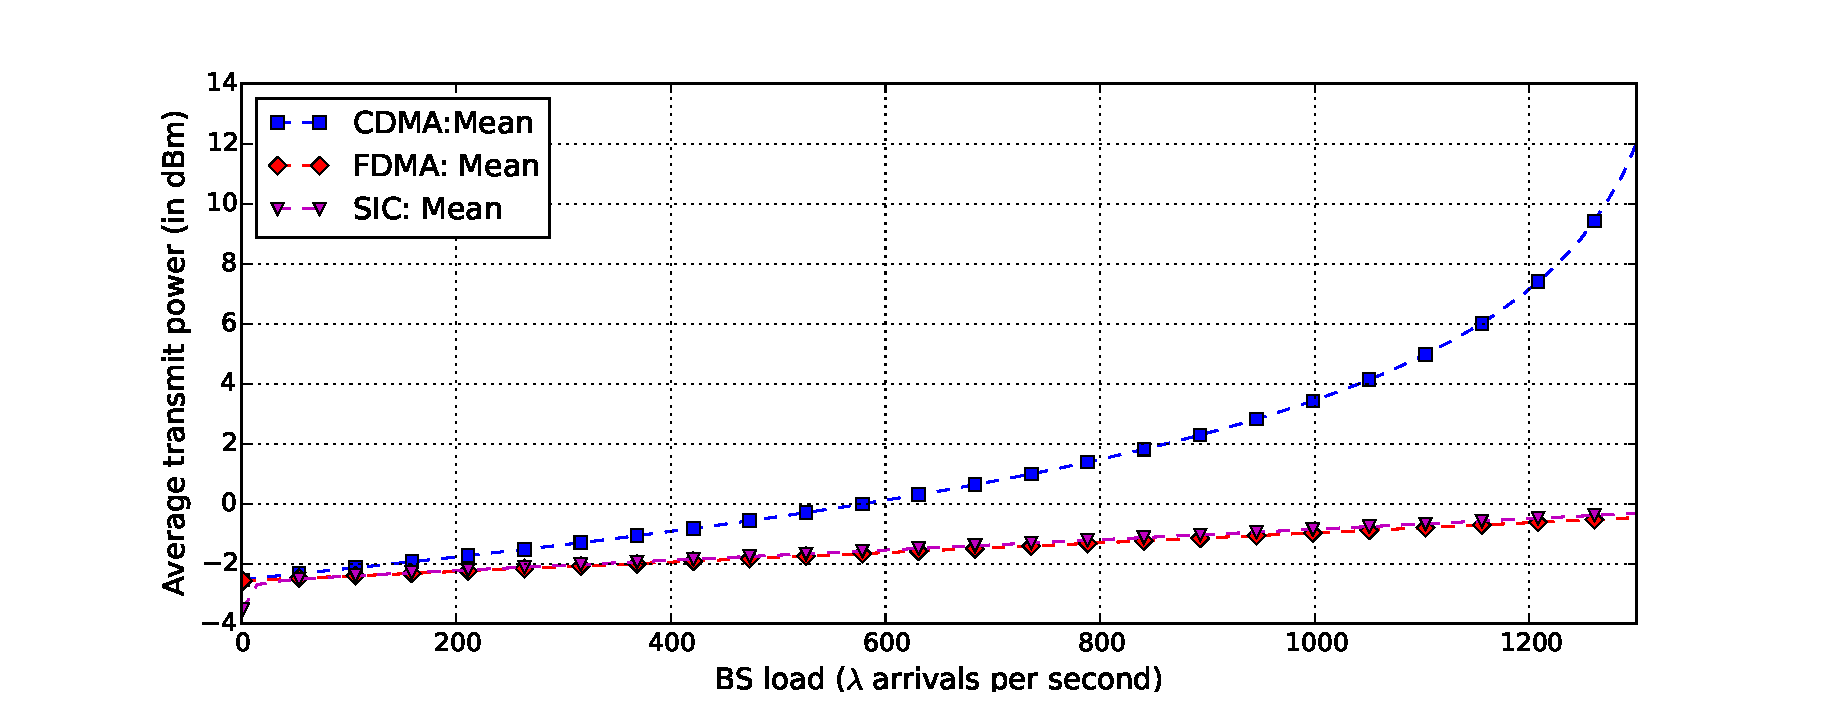
\includegraphics[width=0.5\textwidth, height=5cm]{Figures/Reproduction_Dhillon}
%	\caption{Comparison of power optimal solutions of SIC and FDMA with random access CDMA}
%	\label{fig:comparison-average-transmit-power}
%\end{figure}
\subsection{Impact of various packet length}
As discussed in previous section, the maximum supported base station load intensity is reduced when the maximum packet length increases.
The evolution of maximal packet length as to base station load intensity is illustrated in Fig.~\ref{fig:maximal-packet-length} according to inequality (\ref{ieq:packet-length-interval}). 
We evaluate the average transmit power between FDMA and CDMA under two different configurations where:\begin{inparaenum}[(i)]
	\item the packet length is constant and set as $1000$ bits;
	\item the packet length is variable varying from $1000$ bits to $3000$ bits.
\end{inparaenum}
As shown in Fig.~\ref{fig:maximal-packet-length}, to support a packet length up to $3000$ bits, the maximum base station supported load intensity is reduced to $400$ requests per second. This is the reason why the range of base station load is from $0$ to $400$ in the following figures. The evolution of power efficiency about base station load result is illustrated in Fig.~\ref{fig:Average-Transmit-Power-Variant-Target-SNR}. The curves with label reference case (CDMA or FDMA) respectively refer to the case where packet length payload $l$ is constant (namely $1000$ bits). Among all possible cases, both multiple access strategies achieve the best power efficient performance in reference case. The curve labeled \textit{\emph{CDMA:limit case}} illustrates the case where all MTC devices transfer packets with the length $3L$, which determines the upper bound limit for power consummation. All other possible cases should be between the CDMA limit case and reference case. For example, we assume packet length $l$ as a discrete random variable with distribution: $\mathbb{P}\{l=0.8L\} =0.2, \mathbb{P}\{l=1.0L\} =0.15, \mathbb{P}\{l=1.2L\} =0.15, \mathbb{P}\{l=1.6L\} =0.1, \mathbb{P}\{l=2L\} =0.1, \mathbb{P}\{l=2.5L\} =0.15, \mathbb{P}\{l=3L\} =0.15$, where $L=1000$ bits. The result associated to this configuration is shown by curve with label \textit{\emph{CDMA: general case}}.
From Fig.~\ref{fig:Average-Transmit-Power-Variant-Target-SNR}, we conclude that the coordinated FDMA strategy is more resistant to the variation of the packet length: its average transmit power increases slowly compared to that of CDMA. 

\begin{figure}[hb]
	\centering
	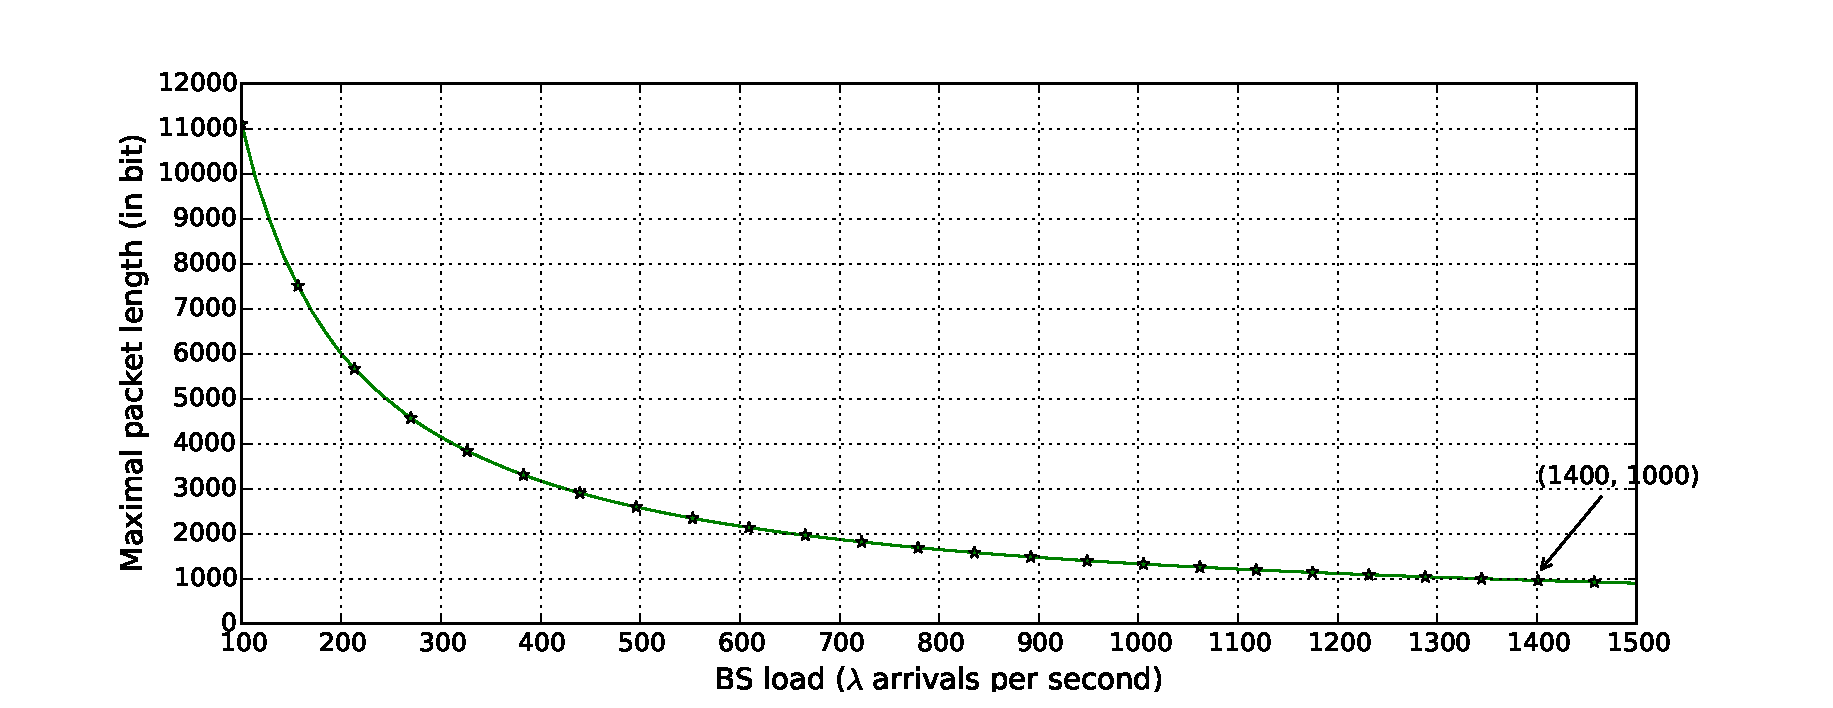
\includegraphics[width=0.5\textwidth, height=5cm]{Chapter3/Figures/Maximal-packet-length-evolution}
	\caption{Evolution of maximal packet length (in bit) with base station load intensity. For maximal packet length of 1000 bits, the maximum supported BS load is 1400.}
	\label{fig:maximal-packet-length}
\end{figure}
\begin{figure}[!tb]
	\centering
	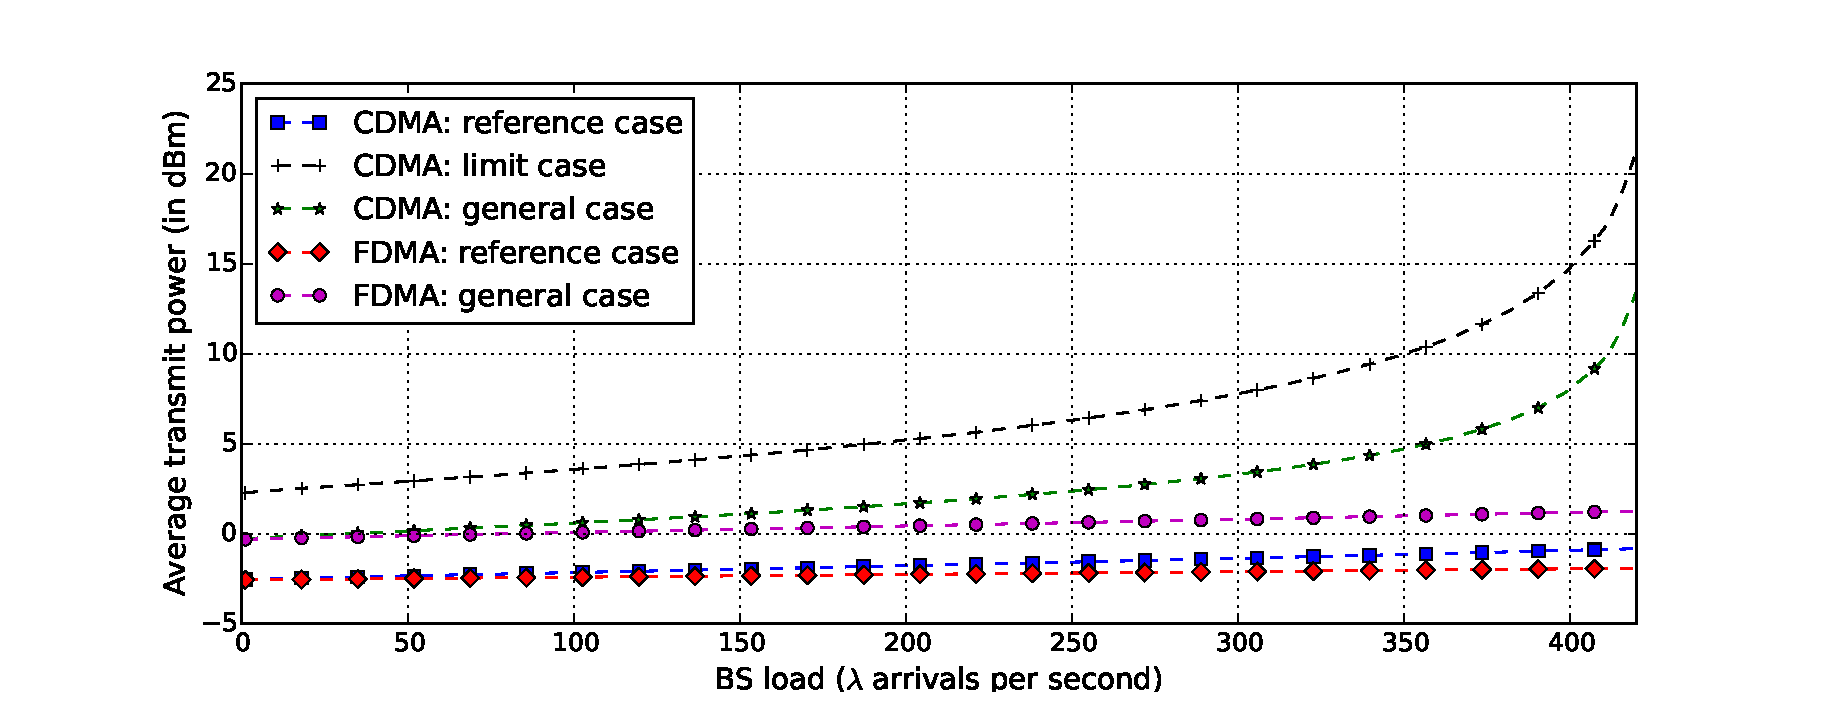
\includegraphics[width=0.5\textwidth, height=5cm]{Chapter3/Figures/Average-Transmit-Power-Variant-Target-SNR}
	\caption{Comparison of average transmit power with various packet length }
	\label{fig:Average-Transmit-Power-Variant-Target-SNR}
\end{figure}
\subsection{Imperfection of power control}
When evaluating the average transmit power under imperfect power control, we assume that the packet length $l$ is constant and set as $1000$ bits. Since it is complicated to obtain the closed-form expression for the term $C$ in formula (\ref{eq:imperfect-CDMA-transmit-power}), we take a statistical method to estimate the average transmit power for each given base station load intensity $\lambda$ and then draw the evolution curve of the average transmit power as a function of the base station load intensity. 
The numerical result where the variance of power control error $\sigma = 1$ is shown in Fig.~\ref{fig:imperfect-power-control-delta1}. The result of power control error variance $\sigma=1, 1.5$ is illustrated in Fig.~\ref{fig:imperfect-power-control-delta2}. 
The blue lines with full squares in both figures represent the case without power control error and thus serves as a reference case. The red scatter points represent the average transmit power with power control error variance $\sigma=1$, while the green scatter points are the case with power control error variance $\sigma=1.5$. From Fig.~\ref{fig:imperfect-power-control-delta1} and \ref{fig:imperfect-power-control-delta2}, the following conclusions are inferred \begin{inparaenum}[i)]
	\item the average transmit power increases when power control is imperfect;
	\item the power efficiency performance has the trend to degrade fast with a high power control error variance $\sigma$ when base station load increases.
\end{inparaenum}
\begin{figure}[!tb]
	\centering
	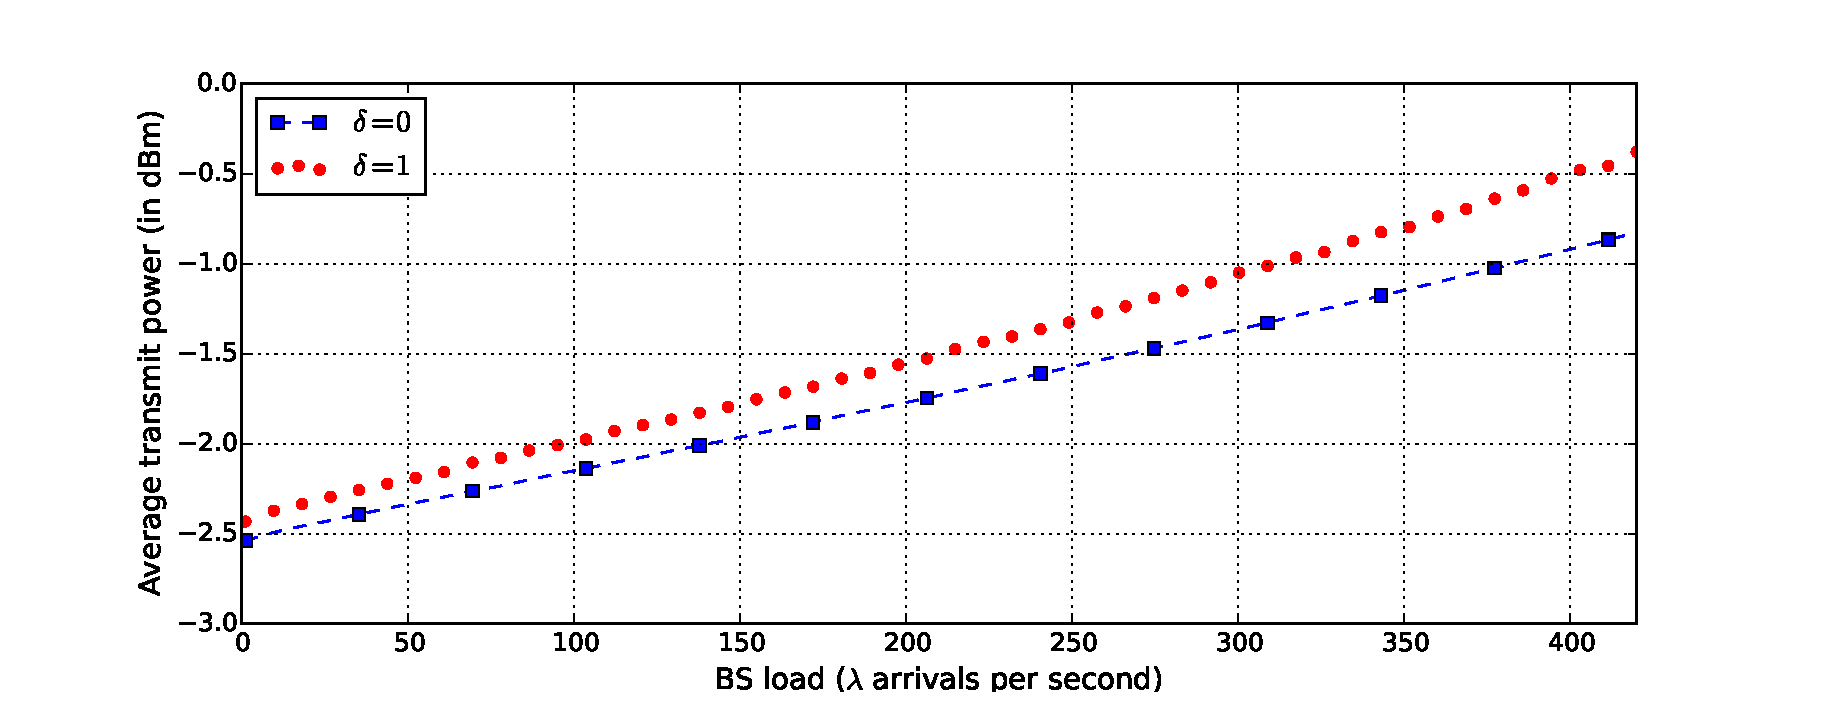
\includegraphics[width=0.5\textwidth, height=5cm]{Chapter3/Figures/Imperfect-power-control-CDMA-delta1-2015-1011}
	\caption{Comparison of average transmit power with power control error of variance $1$ }
	\label{fig:imperfect-power-control-delta1}
\end{figure}
\begin{figure}[!tb]
	\centering
	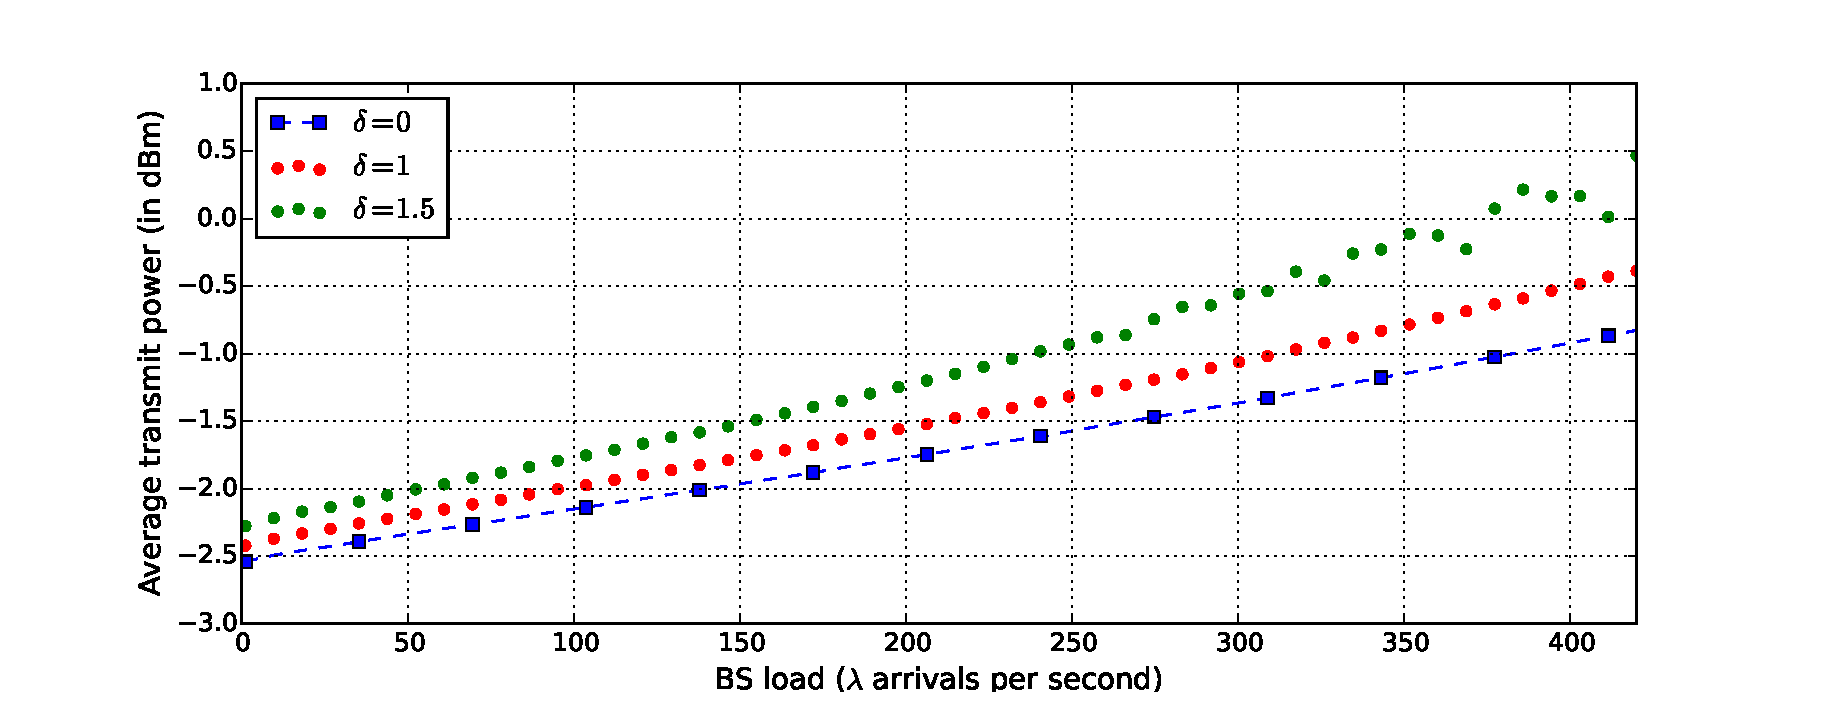
\includegraphics[width=0.5\textwidth,height=5cm]{Chapter3/Figures/Imperfect-power-control-CDMA-delta2-2015-1003}
	\caption{Comparison of average transmit power with power control error of variance $1$ and $1.5$ }
	\label{fig:imperfect-power-control-delta2}
\end{figure}
\section{Conclusion}
\label{sec:conclusion} 
%In this paper, we extend a previously proposed system model by taking into account the impact of variable packet length and the imperfect power control, and reevaluate the energy efficiency and system capacity for two typical multiple access strategies: uncoordinated CDMA and coordinated FDMA. The metric selected for measuring power efficiency is the average transmit power for devices situated in the circle area covered by a single cell. The energy efficiency is measured by the product of time and average transmit power. The system capacity is the maximum supported base station load intensity. The conclusions obtained from the comparison between uncoordinated CDMA and coordinated FDMA are: although uncoordinated CDMA exhibits features such as simplicity and no signaling overhead, it is not always a suitable multiple access for future M2M-included cellular networks. The arguments are following. First, compared with coordinated FDMA, the power efficiency of uncoordinated CDMA performance decreases significantly when BS load intensity increases, especially for the situation where there exist various packet lengths for M2M devices. Second, the power control is very important for the performance of uncoordinated CDMA, but with imperfect power control (which is inevitable in a piratical system), CDMA surely requires a higher level of transmit power, especially when power control error variance is large. Therefore, coordinated access strategy, especially FDMA, can often be a better choice for the future cellular network.
%
%New version:
In this paper, we extend a previously proposed system model by taking into account the impact of variable packet length and imperfect power control, and evaluate the energy efficiency and system capacity for two typical multiple access strategies: uncoordinated CDMA and coordinated FDMA. The metric selected for measuring power efficiency is the average transmit power for devices situated in the circle area covered by a single cell. The energy efficiency is measured by the product of time and average transmit power. The system capacity is the maximum supported base station load intensity. 
The conclusions obtained from the comparison between uncoordinated CDMA and coordinated FDMA are: 
coordinated access strategy, especially FDMA, can often be a better choice for the future cellular network.
Although with power control error, uncoordinated CDMA is a considerable multiple access schema for cellular M2M network dedicated for small data transmission due to its simplicity and no signaling overhead. However, the power efficiency performance of uncoordinated CDMA degrades significantly when BS load intensity increases. Furthermore, the system capacity, namely the maximum supported BS load intensity is rather limited when power control error is obvious.







\chapter{An Analytical Model for S-ALOHA Performance Evaluation of M2M Networks}

% **************************** Define Graphics Path **************************
\ifpdf
    \graphicspath{{Chapter3/Figs/Raster/}{Chapter3/Figs/PDF/}{Chapter3/Figs/}}
\else
    \graphicspath{{Chapter3/Figs/Vector/}{Chapter3/Figs/}}
\fi
Based on ICC2017
\section{Introduction}

\section{State of the Art}

\section{System model}


\section{Ideal system with perfect power control}


\section{Wide-Band Imperfect power control}


\section{System with imperfect power control and Fading}

\section{Summary}





\chapter{Performance Evaluation of ALOHA in context of multiple Base Station}
\label{chapter:ieee-cl-17}

% **************************** Define Graphics Path **************************
\ifpdf
    \graphicspath{{Chapter5/Figs/Raster/}{Chapter5/Figures/PDF/}{Chapter5/Figures/}}
\else
    \graphicspath{{Chapter5/Figs/Vector/}{Chapter5/Figures/}}
\fi

\section{Introduction}
%Machine Type Communication (MTC) is characterized by a large number of terminals, small payload and uplink-centric.
Machine Type Communication (MTC) is expected to gain more popularity in the next decade, which poses great challenges for traditional wireless networks: long range coverage,  low power consumption, access network overload, etc. To tackle with the brought problems,
there are two types of long range MTC systems to handle MTC traffic:\begin{inparaenum}[1)]
 	\item MTC-dedicated networks, also called Low Power Wide Area Network (LPWAN);
 	\item existing cellular networks with adaptations, such as NB-IoT networks~\cite{goursaud2015dedicated}\cite{song2016survey}.
 \end{inparaenum}
For both types of networks, ALOHA plays an important role: either as an initial access method to send a request packet to get resource in cellular networks, or as a data packet transmission method in LPWAN. 
%The MTC-dedicated wireless networks are more attractive faced with MTC specific features~\cite{goursaud2015dedicated}. 

In cellular networks, the packet is sent in unicast mode: the destination Base Station (BS) is indicated by the terminal. However, it also could be sent in broadcast mode, and benefit from macro reception diversity, which is defined as the capacity of several BS to receive the same packet. As for BS, there exist two possibilities to process the received packets. The first one is that each BS autonomously demodulates and decodes the packets (see Fig.~\ref{fig:macro_diversity_recpetion_illustration}). The core network is in charge of duplicate received packets removal (e.g., by comparing the identity and message content conveyed in packets). Such a scheme is presently applied by some LPWAN networks, such as SigFox and LoRaWAN~\cite{ietf-lpwan-overview-03}. The second possibility is that signals received at each BS are linearly combined in the core network so that the output SINR is maximized (see Fig.~\ref{fig:mrc_macro_diversity_recpetion_illustration}). This scheme is like the well-known maximum ratio combining (MRC) technique in Multiple-Input Multiple-Output (MIMO) systems\qsong{Christophe Fourtet said that they were working on combining scheme. I think it's important to give a reference here}. The processing in the core network in both case is out of the scope of this thesis. 
Due to the broadcast nature, the BSs in networks enabling macro reception diversity do not acknowledge the received packets. Hence, the device has to repeat each packet transmission fixed times at random time interval, even if one previous trial is successful. If none of these trials is successful. the packet is lost and the device has no awareness about this.

Not surprisingly, macro reception diversity outperforms the traditional unicast mode in terms of one-shot random access packet loss rate, which means higher system capacity constrained by packet loss rate. However, unicast mode can use retransmission mechanism to reduce packet loss rate while message repeat in macro reception diversity reduces its throughput. The capacity of each mode, which is the maximum supported load for a given packet loss rate target is derived. The ratio between the two capacity values is called the \emph{macro diversity gain}. In this chapter, we give a thorough performance comparison between these two modes, in terms of packet loss rate\qsong{We should use a better metric other than the simple averaged packet loss rate over infinite plane.} , macro diversity gain, throughput\qsong{maybe can consider other metrics...}. We first consider the one-shot random access case and then extend with retransmission mechanism.\qsong{How to include/organize the case of known nearest BS...It's a question...}

%Thus, devices in such networks transmit packets in a ``broadcast`` manner without attach procedure used in cellular networks. SigFox is an example applying the aforementioned macro reception diversity. 
\begin{figure}[!ht]
	\centering
	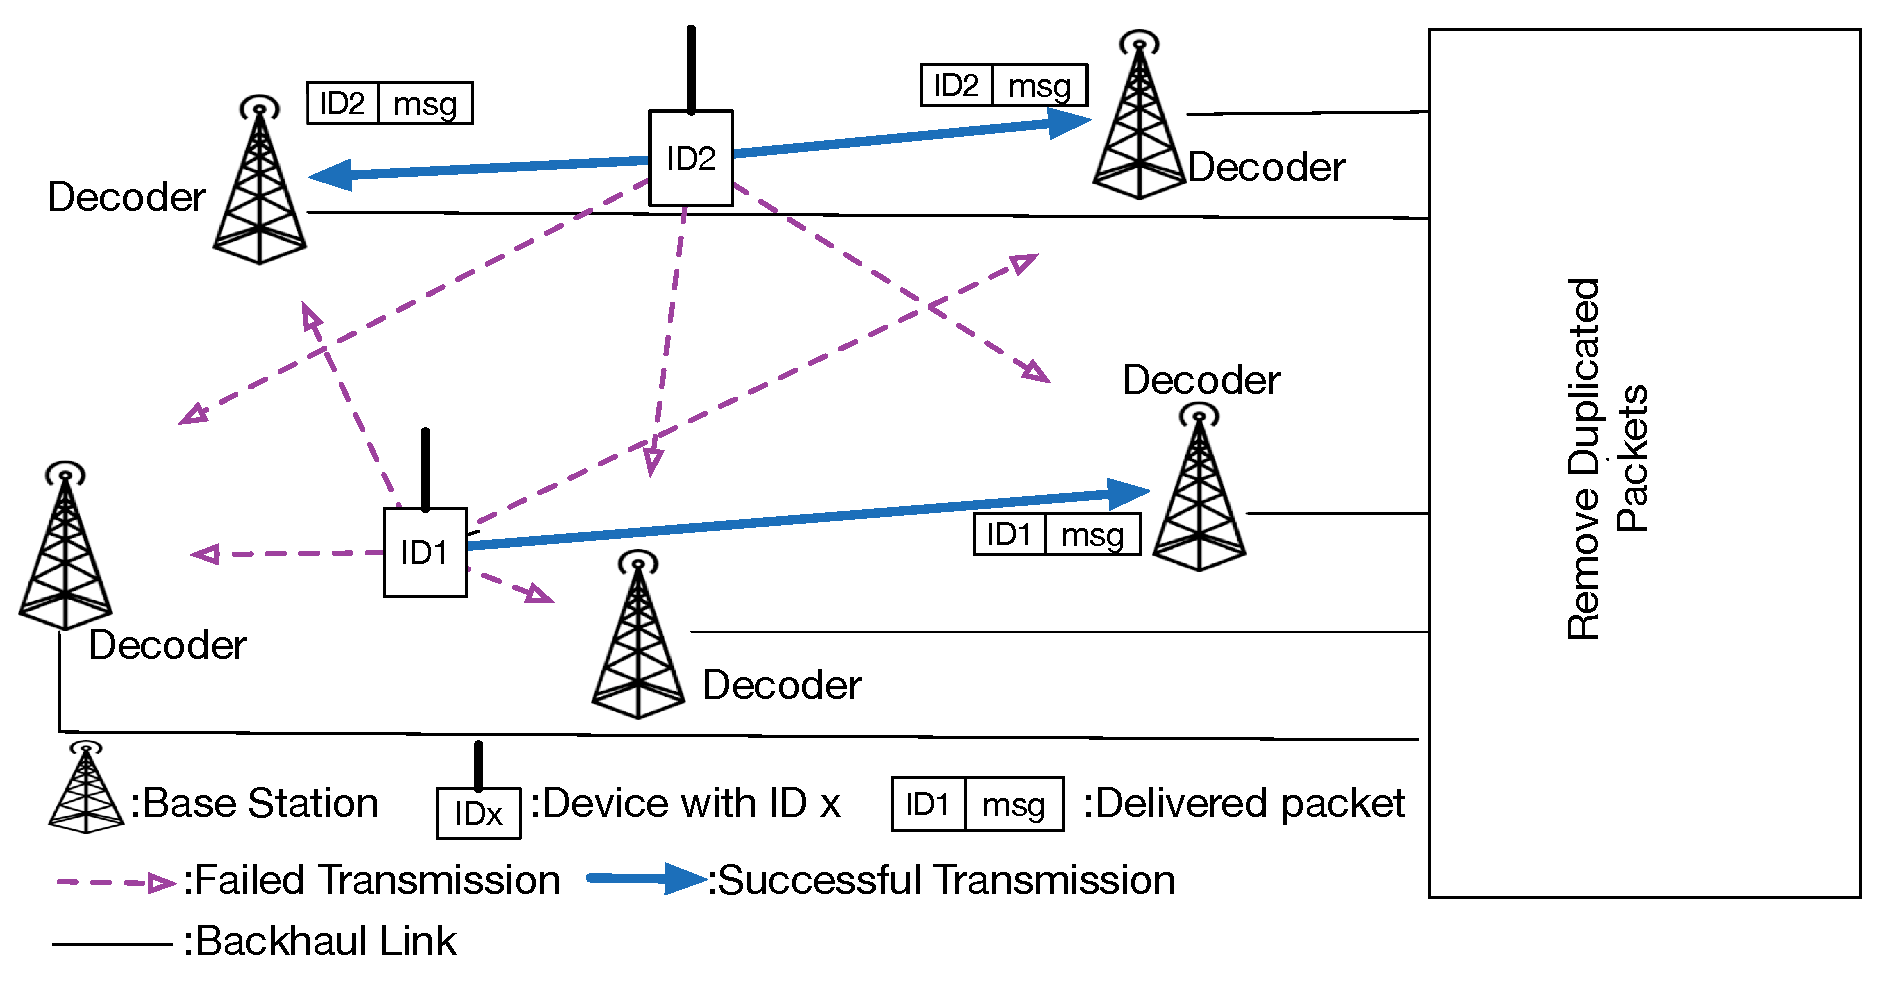
\includegraphics[width=\linewidth]{Chapter5/Figures/Macro_Diversity_Recpetion_Illustration}
	\caption{Macro Reception Diversity Scheme Illustration\qsong{Since we call Maximum Ratio Combining Macro Reception Diversity in anther figure, I'm not sure we should modify the caption of this figure as Selective Combining-like Macro Diversity Reception. Because it is equivalent to judge whether the maximum SINR is greater than captio ratio...}}
	\label{fig:macro_diversity_recpetion_illustration}
\end{figure} 

\begin{figure}[!ht]
	\centering
	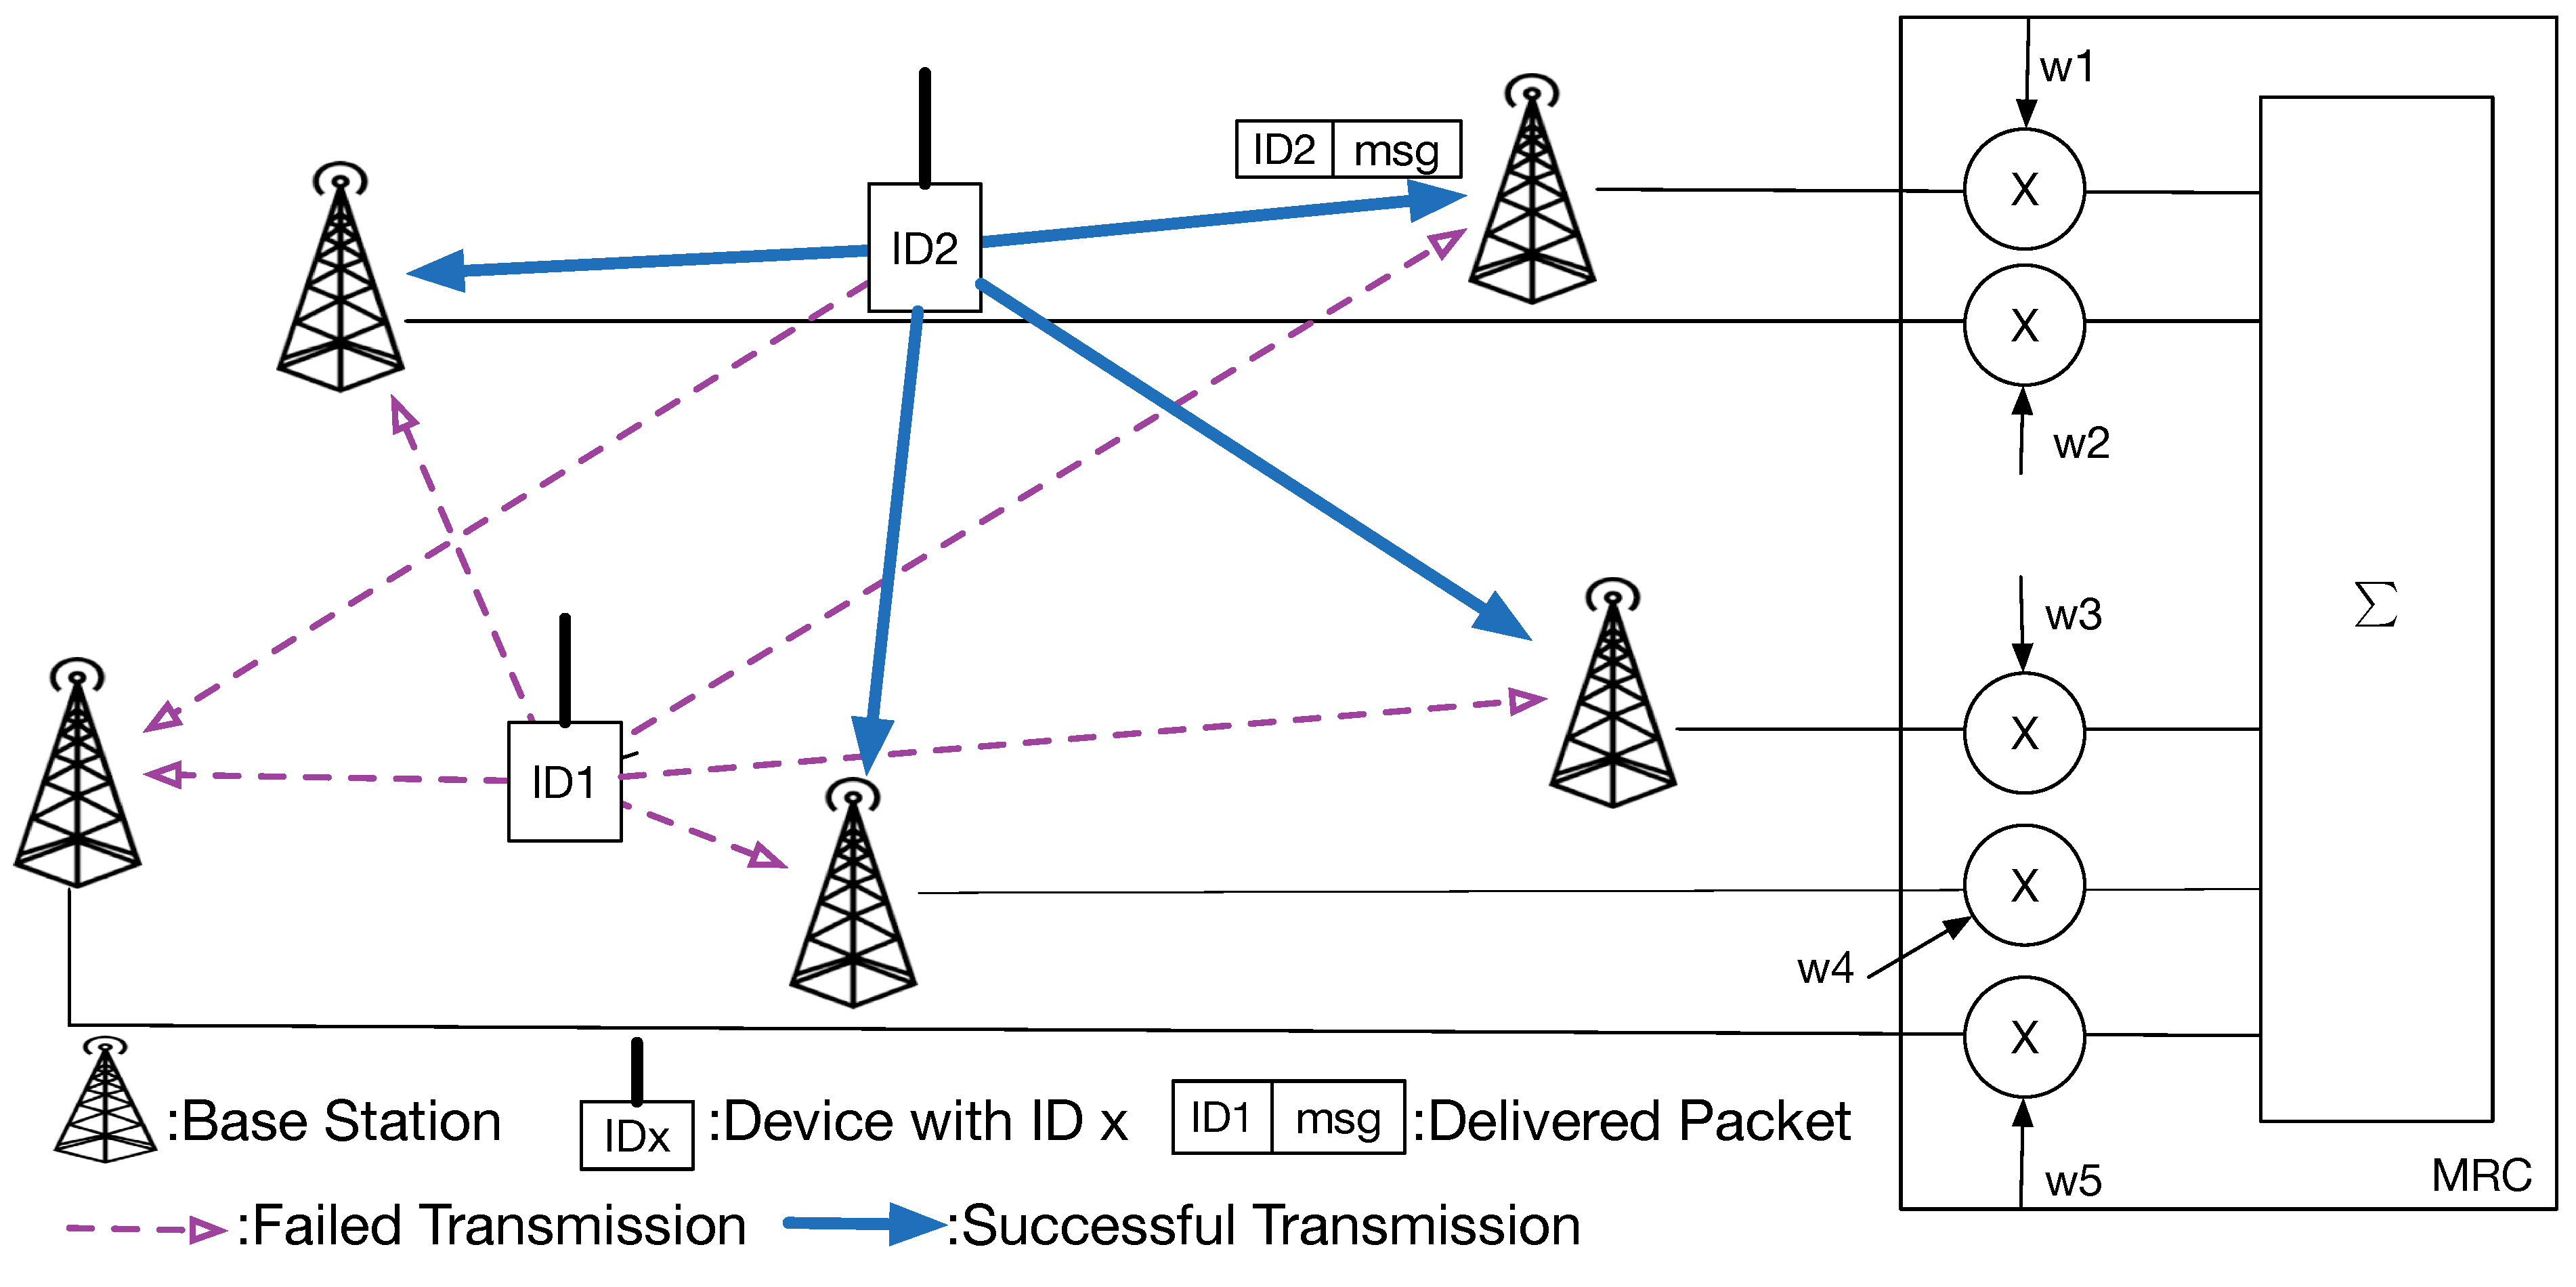
\includegraphics[width=\linewidth]{Chapter5/Figures/MRC_Type_Macro_Diversity_Recpetion_Illustration}
	\caption{Maximum Ratio Combining Macro Reception Diversity Scheme Illustration. The coefficients $w1, w2, ..., w5$ are well designed so that output SINR is maximized.}
	\label{fig:mrc_macro_diversity_recpetion_illustration}
\end{figure} 
%In this broadcast mode, the BSs do not acknowledge the received packets. Hence, the device has to repeat each packet transmission fixed times at random time interval, even if one previous trial is successful. If none of these trials is successful. the packet is lost and the device has no awareness about this. Such a scheme is presently applied by some low-cost dedicated IoT networks, such as SigFox. 

%Not surprisingly, macro reception diversity outperforms the traditional unicast mode in terms of one-shot random access packet loss rate, which means higher system capacity constrained by packet loss rate. However, unicast mode can use retransmission mechanism to reduce packet loss rate while message repeat in macro reception diversity reduces its throughput. 

%In this letter, we propose a simple but accurate analytical model for pure (i.e. non-slotted) and slotted ALOHA based on available stochastic geometry research results. The proposed model takes into account Rayleigh fading, shadowing and capture effect in wireless channel. One can use this model to quantify the macro reception diversity gain in terms of maximum supported load constrained by packet loss rate. 

%derive how many times devices macro reception diversity can serve more that the unicast mode, in a commonly agreed system model. We call the latter performance metric as macro diversity gain.
\section{State of the Art
% TODO: the related work part is not enough detailed. To be detailed afterwards.
%	\qsong{to be detailed...}
}
In literature, the performance of ALOHA-based LPWAN are usually analyzed with Stochastic geometry. Baccelli et al.~\cite{baccelli2006aloha} use Laplace transform for interference analysis for slotted ALOHA. Haenggi et al.~\cite{haenggi2009interference} extensively study the outage probability in SINR-based capture model for slotted ALOHA. B{\l}aszczyszyn et al.~\cite{blaszczyszyn2010stochastic} open the door to study pure ALOHA with stochastic geometry. However, to our best knowledge, macro reception diversity for ALOHA systems has not been studied in literature.
\section{System model}
\label{sec:system_model}
% Xavier's suggestion:
%	Plus précisément, ce qui me semble intéressant c'est de comprendre l'évolution des performances pour 3 configurations
%- Slotted Aloha avec transmission à la meilleure BS et avec une voie de retour (type réseau cellulaire)
%- Pure Aloha avec macro-diversité et une voie de retour (type LORA)
%- Pure Aloha avec macro-diversité sans voie de retour (type LORA)
\subsection{Distribution of Nodes and Traffic Model}
We consider a large wireless network over a two-dimension infinite plane. The locations of terminals form a stationary Poisson point process (PPP) $\Phi_m = \left\lbrace X_i\right\rbrace$ on the plane $\mathbb{R}^2$ with spatial density $\lambda_m$.  Similarly, the locations of base stations also form a stationary PPP $\Phi_b = \left\lbrace Y_i\right\rbrace$ with spatial density $\lambda_b$. One devices and BSs spatial distribution realization is shown in Fig.~\ref{fig:device_BS_spatial_distribution}. All the packets transmitted by devices have the same duration $B$.
\begin{figure}[!ht]
	\centering
	\includegraphics[width=\linewidth]{/Users/qsong/Documents/slotted_aloha_related_project/multiple_recepteur_capacity/nodes_spatial_dist.eps}
	\caption{Maximum Ratio Combining Macro Reception Diversity Scheme Illustration. The coefficients $w1, w2, ..., w5$ are well designed so that output SINR is maximized.}
	\label{fig:device_BS_spatial_distribution}
\end{figure} 

\subsection{Slotted ALOHA and Pure ALOHA}
For a comparison between macro reception diversity and traditional BS attach method, we consider three types of ALOHA-based network. As a comparison reference, we consider a traditional cellular network which employs slotted ALOHA. The devices in such a network attach to its best BS for which the received power averaged over all fading realizations is the strongest. For macro reception diversity, it is assumed to run in pure slotted ALOHA. Furthermore, this networks with macro reception diversity can be divided into two categories: with downlink for acknowledgment (e.g. LoRaWAN) and without downlink for acknowledgment (note that SigFox has downlink support but does not use it for acknowledgment). Note that whether acknowledgment is supported has an impact on retransmission mechanism. 

For slotted ALOHA, the time domain is equally divided into slots with duration $B$. In each slot, each device independently decides to transmit a packet with probability $p$. The propagation delay is assumed to be much smaller than $B$. Hence, there is a global slot synchronization over the whole network.

In pure ALOHA, devices send packets without synchronization, but we still use parameter $p$. The packet generation process can be seen as an internal slotted system in each device with $p$ the probability to transmit in a slot of duration $B$.

At a given time, the locations of terminals that are transmitting a packet form a PPP with spatial density $p\lambda_{m}$. For slotted and pure ALOHA, we define the normalized load (per BS) as $L = p\lambda_{m}/\lambda_{b}$. In addition, we just consider one-shot random access. This model can be easily extended with retransmission mechanisms.
\subsection{Random Channel and Capture Effect}
% Xavier insists that this is a communication letter which should be concise.
% Not necessary to explain somethings well-known for readers with enough background knowledges.
We assume that M2M devices do not support power control mechanism due to the low-cost constraint and transmit with unit power level. M2M-dedicated networks are usually narrow band and thus can be assumed to suffer Rayleigh fading. For example, NB-IoT use $180$ kHz bandwidth~\cite{wang2017primer} and SigFox's bandwidth is $100$ Hz~\cite{raza2017low}. The bandwidth of $LoRaWAN$ varies from $125$ kHz to $500$ kHz according to different spread-spectrum sequence. Although LoRaWAN applies spectrum spreading technology, it can still be assumed to suffer Rayleigh fading~\cite{georgiou2017low} in literature.
Thus, the received power $P_{r}$ of a packet at the base station side depends on path-loss attenuation $r^{-\gamma}$, Rayleigh fading $H$ and shadowing effect $\exp(\chi)$:
\begin{align}
\label{eq:path-loss}
P_{r} =d^{-\gamma} H \exp(\chi),
\end{align}
%The path-loss attenuation $l(r)$ is defined as $l(r) = r^{-\gamma}$, 
where $d$ refers to the distance between the transmitter and the receiver, $\gamma$ is the path-loss exponent, $H$ is an exponentially distributed random variable (r.v.) with unit mean, $\chi$ is a zero-mean Gaussian r.v. with variance $\sigma^2$. Log-normal shadowing is usually characterized in terms of its dB-spread with standard deviation $\sigma_{dB} = \frac{10}{\ln(10)}\sigma$. We assume that $H$ and $\chi$ are both constant during a packet transmission, and mutually independent for different links. 
%Due to channel randomness, it is possible that the received power at a far device is stronger than a close device. 

\subsection{Displacement theorem and transformed PPP}
\label{subsec:displacement_theorem}
As mentioned in Sec.~\ref{sec:system_model}, each device is assumed to connect to the BS that provides the highest long-term biased received power. The inclusion of shadowing allows to rewrite $\eqref{eq:path-loss}$ as follows:
\begin{align}
P_{r} 
&= H \left[  \exp^{-1/\gamma}(\chi) d \right]  ^ {-\gamma},
\end{align}
where shadowing can be interpreted as a random displacement of the location of BS. This fact can be leveraged by using displacement theorem~\cite{franccois2009stochastic}. That is to say, attaching to the best BS in a PPP of intensity $\lambda_{b}$ with shadowing is equivalent to attaching the geographically nearest one in a transformed PPP of intensity $\lambda_{b} \mathbb{E}\left[ e^{-\frac{2}{\gamma}\chi}\right] = \lambda_{b} e^{\frac{2\sigma^2}{\gamma^2}}$ without shadowing. This lemma is given in~\cite[lemma 1]{dhillon2014downlink} and detailed proof is given in~\cite[Corollary 3]{madhusudhanan2014downlink}. We use $r$ to denote the distance between device and BS in the transformed PPP.

%Capture effect refers to the fact that signals in collision can still be demodulated if their received SINR are greater than or equal to a certain threshold value. 
Capture effect is taken into account in the proposed model. Thus, the transmission success probability $p_{s}$ for a transmit-receiver pair is defined as follows: 
\begin{align}
\label{eq: sinr-definition}
p_s = \mathbb{P}\left\lbrace  \text{SINR} = \frac{P_r}{I + N} \geq \theta_{T} \right\rbrace, 
\end{align}
where $I$ refers to the suffered cumulative interference during packet transmission, $N$ is the normalized background noise power. It is worthwhile to mention that in some cases the background noise is rationally negligible for the sake of tractability.

\subsection{Impact of background noise}
Actually, the background noise is usually neglected in the study of LPWAN system. One institutive exposition about this is that the occupied transmission bandwidth is small and the noise power is at a low level. Here, we give an estimation about the normalized noise power value $N$ if transmit power is assumed to be $1$. To this end, we have to know, in a realistic LPWAN network, the ratio between the received power and the real background noise level.

For one LPWAN device running on ISM band (e.g. with 868 MHz), from a regulatory point of view, the effective radiated power (ERP) may not exceed $14$ dBm (or $25$mW) in any direction, we thus assume that the transmit power is set as $14$ dBm.

About noise power level, we use the same formula given in~\cite{georgiou2017low}:
\begin{align}
	N_{\textbf{real}} = -174 + NF + 10\log(W) ,
\end{align}
where $NF$ is noise figure, usually set as $6$dB, $W$ is the bandwidth occupied by the transmitted packet. The occupied transmission band is assumed to be between $100$ Hz and $200$ KHz. Thus, the possible value of $N_{\text{real}}$ is between $-148$ dBm and $-115$ dBm.

In terms of propagation path-loss model, Okumura-Hata model is applied. In urban area, the path-loss between one device and a BS with height $50$ meters is~\cite{lagrange2000reseaux}:  
\begin{align}
	\text{Path_Loss}= 123.6+33.8\log(d),
\end{align}
where $\log(\cdot)$ is $10$-based logarithm operator.

Therefore, if we assume that transmit power is $1$, the normalized noise power $N$ should take values in range $\left[ -38.4, -5.4\right] $. 
%According to the simulation that we have conducted, 



%\subsection{Performance Metric}
%\subsubsection{Packet loss rate}
%xxx
%\subsubsection{Macro Diversity Gain}
%xxx
%\subsubsection{Throughput}
%xxx
%\subsubsection{Energy efficiency}
%xxx
%Similarly, we also consider two different ways to estimate interference with respect to device coding schemes. If no interleaving and error correction code technique are not used, the cumulative interference is the maximal interference value during the transmission B: $I^{\text{max}} = \max I(t)$ for $t \in \left[ T, T+B\right] $. If advanced techniques to resistant transmission error are used, average interference over the packet transmission $I^{\text{mean}} = \frac{1}{B}\int_{T}^{T+B} I(t)dt$.

%Empirical measurements shows that shadowing effect, when represented in dB units, follows a normal distribution (see e.g.\cite{erceg1999empirically}). In other words, the linear (as opposed to dB) channel gain may be modeled by a log-normal random variable, $e^G$, where $G$ is a zero-mean Gaussian r.v. with variance $\sigma^2$. Log-normal shadowing is usually characterized in terms of its dB-spread, $\sigma_{dB}$, which is related to $\sigma$ by $\sigma = \frac{\ln(10)}{10}  \sigma_{dB}$. Thus, The received power $P_{r}$ is expressed as follows:

%As to the non-slotted ALOHA protocol, we still divide the time domain into slot of length $B$, one packet appears with probability $p$ in a given slot, but the packet arrival time is not the beginning of a slot like in slotted ALOHA. Instead, packet arrival time is uniformly distributed in a slot. 

%At a given time, the locations of terminals that are transmitting a packet form a PPP with spatial density $p\lambda_{m}$. A BS can correctly receive at most one packet at a given time. 
%For slotted and pure ALOHA, we define the normalized load (per BS) as $p\lambda_{m}/\lambda_{b}$. In non-overload conditions, $p\lambda_{m}/\lambda_{b} < 1$.













\section{Link-level Transmission Success Probability}
\label{sec:trans_succ_p_pair}
We first study the transmission success probability $p_s(r)$ for a given uplink between a BS at the origin and a device $x_0$ at distance $r$. Using Slivnyak's theorem~\cite{vaze2015random}[Theorem 2.3.3], combining $(\ref{eq:path-loss})$ and $(\ref{eq: sinr-definition})$, we have:
\begin{align}
p_{s} \left( r\right)
& =\mathbb{P}\left\lbrace \frac{H \exp(\chi) r^{-\gamma}}{\sum_{x_j \in \Phi_{m}} H_{x_j} \exp(\chi_{x_j}) r_{x_j}^{-\gamma}}  \geq \theta_T \right\rbrace. \nonumber
\end{align}
Let $I=\sum_{x_j \in \Phi_{m}} H_{x_j} \exp(\chi_{x_j}) r_{x_j}^{-\gamma}$, which is the cumulative interference suffered by $x_0$. Conditioned on log-normal shadowing component $\exp(\chi_{x_j}) $, as shown in~\cite{haenggi2009interference}, $p_{s}\left( r \right)$ can be expressed in terms of Laplace transform of cumulative interference $\mathcal{L}_{I}(s)$ at point $\theta_{T} e^{-\chi} r^{\gamma}$:
\begin{align}
\label{eq:def_ps}
p_{s}\left( r \right)  &= Pr \left\lbrace H  \geq I \theta_{T} e^{-\chi}r ^{\gamma}  \right\rbrace \nonumber\\ 
% The follwing line can be hidden, not necessary in FINAL_VERSION
%&=\mathbb{E}_{\chi}\left\lbrace  \mathbb{E}_{I} \left[ \exp(-\theta_{T} \exp(-g) r^{\gamma}  I ) \vert \chi = g\right]\right\rbrace   \nonumber\\
&= \int_{-\infty}^{+\infty} \left[ \int_{0}^{+\infty} \exp(-y \theta_{T} e^{-x} r^{\gamma} ) f_{I}(y)dy\right] f_{\chi}(x) dx  \nonumber\\
&= \mathbb{E}_{\chi} \left[ \mathcal{L}_{I}\left\lbrace \theta_{T} e^{-\chi} r^{\gamma}\right\rbrace \right],
\end{align}
where $f_{X} (x)$ is probability density function (PDF) of r.v. $X$, $\mathbb{E}_{X} \left[ \cdot \right] $ is the expectation operator with respect to $X$.
\subsection{Slotted ALOHA}
In slotted ALOHA, the cumulative interference is constant during each slot. The geometry-aware interference analysis for slotted ALOHA is well investigated. Reference~\cite{haenggi2009interference} gives a closed-form expression about the Laplace transform of cumulative interference. With independent Rayleigh fading and log-normal shadowing, we have:
\begin{align}
\label{eq:lp_tr_slotted}
%\mathcal{L}_{I}\left( s \right) &=\exp\left\lbrace -p\lambda_m K_{\text{slotted}} \mathbb{E}\left[ H^{\frac{2}{\gamma}}\exp(\frac{2}{\gamma}\chi)\right]s^{\frac{2}{\gamma}}  \right\rbrace
\mathcal{L}_{I}\left( s \right)  &=\exp \left\lbrace
-p\lambda_m \pi A  \exp \left( 2\sigma^2/\gamma^2\right) s^{2/\gamma}  
\right\rbrace,
\end{align}
where $A = \Gamma(1-\frac{2}{\gamma})\Gamma(1+\frac{2}{\gamma})$ and $\Gamma(z)=\int_{0}^{+\infty} x^{z-1} e^{-x} dx$. 
%is called the spatial contention factor~\cite{haenggi2009outage}, $\Gamma(z)$ is the gamma function defined as $\Gamma(z)=\int_{0}^{+\infty} x^{z-1} e^{-x} dx$. 
%Since $H$ and $\chi$ are independent, $\mathbb{E}\left[ H^{\frac{2}{\gamma}}\exp(\frac{2}{\gamma}\chi)\right] = \Gamma(1+\frac{2}{\gamma}) \exp \left( \frac{\sqrt{2}\sigma}{\gamma}\right) ^2$.
\subsection{Pure ALOHA}
\label{subsec: pure-aloha}
In pure ALOHA, the cumulative interference $I(t)$ suffered by a given packet transmitted in interval $\left[ T, T+B\right]$ is variable during the packet transmission. When advanced transmission techniques (e.g., interleaving, robust channel coding, etc.) are used, $p_{s}(r)$ is a function of the average interference $I^{\text{mean}} = \frac{1}{B}\int_{T}^{T+B} I(t)dt$, which replaces $I$ in $(\ref{eq: sinr-definition})$.

B{\l}aszczyszyn et al. propose a Poisson-rain model~\cite[Sec.2.4]{blaszczyszyn2015interference} that approximates well this case and allows to compute the cumulative interference. They prove that formula $(\ref{eq:lp_tr_slotted})$ can be reused by letting $A=\frac{2\gamma}{\gamma + 2} \Gamma(1-\frac{2}{\gamma})\Gamma(1+\frac{2}{\gamma})$.
%\subsection{Pure ALOHA, maximum interference}

Another case of pure ALOHA is assumed to have no error correction neither interleaving techniques for the purpose of reducing the device-side cost. In this case, the packet is delivered if and only if each bit is correctly received. Hence, the SINR should be larger than or equal to $\theta_{T}$ during $B$. Hence, $p_{s}$ is a function of maximum interference $I^{\text{max}} = \max_{t \in \left[ T, T+B\right]} I(t)$. According to~\cite[Sec.2.4]{blaszczyszyn2015interference}, there is no closed-form for $I^{\text{max}} $, and the authors use a simulation approach to study. Next, we propose a simple upper bound to estimate $I^{\text{max}}$. Section~\ref{sec:simulation} shows that the bias is at an acceptable level.

Consider a packet transmitted in interval $\left[ T, T+B\right]$. Any device generating its interference at $T$ terminates packet transmission before $T+B$. The interfering packets at $T+B$ do not exist at $T$, because the packet transmission duration is $B$. 
Hence, cumulative interference $I(T)$ and $I(T+B)$ are two independent and identically distributed random variables. Furthermore, any device generating interference on the packet is either active at $T$  or at $T+B$. The maximum interference is thus upper bounded by $I(T)+I(T+B)$. Therefore, the Laplace transform of maximum cumulative interference upper bound $\mathcal{L}_{I^{\text{upper}}}\left( s \right)$ during interval $\left[ T, T+B\right]$ is equal to $ \mathcal{L}_{I(T)+I(T+B)}\left( s\right)= \left[ \mathcal{L}_{I(T)}\left( s\right) \right]^2$. 

We can reuse $(\ref{eq:lp_tr_slotted})$ to calculate $\mathcal{L}_{I(T)}\left( s\right)$. Thus, Laplace transform of $I^{\text{upper}}$ can be unified into $(\ref{eq:lp_tr_slotted})$ by letting $A=2 \Gamma(1-\frac{2}{\gamma}) \Gamma(1+\frac{2}{\gamma})$. 

Combining $(\ref{eq:def_ps})$ and $(\ref{eq:lp_tr_slotted})$, we can express $p_s(r)$ with a formula common to all ALOHA cases:
\begin{align}
\label{eq:def_ps_2}
p_{s}(r) & = \mathbb{E}_{\chi}\left[ \exp(-p \lambda_{m} \pi A \theta_{T}^{\frac{2}{\gamma}} e^{\frac{2\sigma^2}{\gamma^2}}  r^2 e^{-\frac{2}{\gamma}\chi}) \right],
\end{align}
%\begin{align}
%\label{eq:conditional_lp_trans}
%\mathcal{L}_{I}\left\lbrace \theta_{T} \exp(-\chi) r^{\gamma}\right\rbrace = \exp\left\lbrace -A K r^2\exp(-\frac{2}{\gamma}\chi)\right\rbrace,
%\end{align}
where $\sigma = \frac{\ln(10)}{10}\sigma_{dB}$ and:
\[ \!\!\!\!A =
\begin{cases} 
\Gamma\!\!\left( 1-\frac{2}{\gamma}\right)\Gamma\!\!\left( 1+\frac{2}{\gamma}\right) ,  & \text{for slotted ALOHA }\\
\frac{2\gamma}{\gamma+2}\Gamma\!\!\left( 1-\frac{2}{\gamma}\right)\Gamma\!\!\left( 1+\frac{2}{\gamma}\right),  & \parbox[t]{.41\columnwidth}{for pure ALOHA, average interference }\\
2\Gamma\!\!\left( 1-\frac{2}{\gamma}\right)\Gamma\!\!\left( 1+\frac{2}{\gamma}\right),  & \parbox[t]{.4\columnwidth}{for pure ALOHA, maximum interference }
\end{cases}
\]
%With substitution of $(\ref{eq:conditional_lp_trans})$ into $(\ref{eq:def_ps})$, 
%Although expression $(\ref{eq:def_ps_2})$ is not in closed-form, it simplifies the analysis in Sec.~\ref{sec:op_over_infinite_plane}. 

%The authors of paper: Interference and SINR coverage in spatial non-slotted ALOHA networks, state that: We have not been able to derive closed formulas when the maximal interference constraint is used; this case is studied by simulations in Section 5.

%\[ \!\!\!\!K\!\!\!=\!\!\!
%\begin{cases} 
%\pi \Gamma\left( 1-\frac{2}{\gamma}\right),  & \text{for slotted ALOHA }\\
%\frac{2\gamma\pi}{\gamma+2}\Gamma\!\!\left( 1-\frac{2}{\gamma}\right),  & \parbox[t]{.41\columnwidth}{for pure ALOHA, average interference }\\
%2\pi \Gamma\left( 1-\frac{2}{\gamma}\right),  & \parbox[t]{.4\columnwidth}{for pure ALOHA, maximum interference }
%\end{cases}
%\]
%
%\[ K\!\!\!=\!\!\!
%\begin{cases} 
%\pi \Gamma\left( 1-\frac{2}{\gamma}\right),  & \text{for slotted ALOHA }\\
%\!\!\frac{2\gamma\pi}{\gamma+2}\Gamma\!\!\left( 1-\frac{2}{\gamma}\right),  & \!\!\!\text{for pure ALOHA, average interference}\\
%\!\!2\pi \Gamma\!\!\left( 1-\frac{2}{\gamma}\right),  & \!\!\!\!\!\!\!\text{for pure ALOHA, maximum interference }
%\end{cases}
%\]
\section{Performance Without Retransmission}
\label{sec:op_over_infinite_plane}
The transmission success probability $p_s(r)$ paves the way to analyze the network packet loss rate $P_{f}$, which is the base to calculate:\begin{inparaenum}[1)]
	\item the maximum normalized load $L_{\text{max}}$ under packet loss rate constraint $P_{f}^{\text{max}}$;
	\item the normalized spatial throughput (per BS) $S = (1-P_{f}) p\lambda_{m}/ \lambda_{b}$
\end{inparaenum}
We first consider two standard ALOHA transmission approaches in unicast mode (best and nearest BS attach) and then analyze the macro diversity case. For macro diversity case, we also consider two cases: selective ratio and maximum ratio combing.
\subsection{Nearest BS attach method}
\label{sec:nearest_BS_attach_method}
%A device can attach to the best BS which the received power of packet transmission is the strongest if the channel state info is available during the communication.
In this subsection, we assume that the device attaches to the geographically nearest BS then transmits packets. 
%This method is rational when downlink is seldom used for the sake of cost. %TODO: Add this in cover letter.
Therefore, network packet loss rate $P_{f,n}$ (index $n$ means nearest) is the expectation of $p_s(r)$ with respect to the distance to the nearest base station $r$ . The PDF of $r$ for a PPP, proved in~\cite{andrews2011tractable}, is as follows:
\begin{align}
\label{eq:pdf_nearest_distance}
f\left( r\right)  = 2 \pi \lambda_b  r \exp(-\lambda_b \pi r^2), r \in \left[ 0, +\infty\right]. 
\end{align}
Thus:
\begin{align}
\label{eq:mean_bx+1_step1}
&P_{f,n}= \mathbb{E}_{r}\left[ 1-p_{s}\left(r\right) \right]  \nonumber\\
&= 1 -\int_{0}^{+\infty} \mathbb{E}_{\chi} \left[ \exp(-p \lambda_{m} \pi A \theta_{T}^{\frac{2}{\gamma}} e^{\frac{2\sigma^2}{\gamma^2}}  r^2 e^{-\frac{2}{\gamma}\chi}) \right] 2 \pi \lambda_b  r e^{-\lambda_b \pi r^2} dr \nonumber\\
&= 1-\pi \lambda_b \mathbb{E}_{\chi}\left[ \int_{0}^{+\infty} \exp(-p \lambda_{m} \pi A \theta_{T}^{\frac{2}{\gamma}} e^{\frac{2\sigma^2}{\gamma^2}}  r^2 e^{-\frac{2}{\gamma}\chi}-\lambda_b \pi r^2)\right] \!\!dr^2 \nonumber\\
&= 1 -\mathbb{E}_{\chi}\left[\left( A \theta_{T}^{\frac{2}{\gamma}} e^{\frac{2\sigma^2}{\gamma^2}} L  e^{-\frac{2}{\gamma}\chi}+1 \right)^{-1} \right] \nonumber\\
%&= 1- \int_{-\infty}^{+\infty} \frac{1}{ \frac{p\lambda_{m}AK}{\pi \lambda_{b}}e^t+1}\frac{\exp\left\lbrace -\frac{t^2}{2 \left( \frac{2}{\gamma}\sigma\right) ^2}\right\rbrace }{\sqrt{2\pi} \frac{2}{\gamma}\sigma} dt \nonumber\\
&= 1 - \int_{-\infty}^{+\infty} \!\!\! \frac{\gamma}{ 2\sqrt{2\pi}\left( e^t+1\right)\sigma} \exp \left\lbrace -\frac{\gamma^2}{8 \sigma^2} \left(    t-\ln(A L \theta_{T}^{\frac{2}{\gamma}} e^{\!\! \frac{2\sigma^2}{\gamma^2}} )   \right) ^2 \right\rbrace dt.  
\end{align}
%which is actually a logistic-normal integral. According to~\cite{crooks2009logistic}, this kind of 
Integral in $(\ref{eq:mean_bx+1_step1})$ can be accurately approximated by a logistic function~\cite{crooks2009logistic}. Thus,
\begin{align}
\label{eq:bs_nst_att_analytical}
P_{f,n} 
&\approx 1 - \frac{1}{1 + \exp\left\lbrace \left( 1 +\pi \sigma^2 / (2\gamma^2) \right)^{-1/2} \ln( A \theta_{T}^{\frac{2}{\gamma}} e^{\frac{2\sigma^2}{\gamma^2}}  L) \right\rbrace}  \nonumber\\
&\approx 1-\frac{ 1 }{ 1 + \left( A \theta_{T}^{\frac{2}{\gamma}} e^{\frac{2\sigma^2}{\gamma^2}}  L\right) ^{C} }
\end{align}
where $A$ is defined in $(\ref{eq:def_ps_2})$, $L=p\lambda_{m}/\lambda_{b}$, $C= \left( 1 +\pi \sigma^2 / (2\gamma^2) \right)^{-1/2}$. We conducted a Monte-Carlo simulation and found that the maximum difference between $(\ref{eq:mean_bx+1_step1})$ and $(\ref{eq:bs_nst_att_analytical})$ is $2.46\%$ in normalized load interval $\left[ 0.021, 0.3\right] $, which proves the accuracy of the proposed approximation formula $(\ref{eq:bs_nst_att_analytical})$\qsong{Remember to put the figure into Annexe part. Here I wan to show that, the difference between approximation formula and exact integral is smaller when normalized load increase }.
\begin{figure}[!ht]
	\centering
	
\includegraphics[width=\linewidth]{/Users/qsong/Documents/slotted_aloha_related_project/test/comparison_monte_carlo_approximation.eps}
	\caption{Comparison between approximation formula $(\ref{eq:bs_nst_att_analytical})$ and Monte-Carlo simulation result.}
	\label{fig:comparison_monte_carlo}
\end{figure}

From $(\ref{eq:bs_nst_att_analytical})$,  the maximum supported normalized load $L_{\text{max},n}$ and normalized spatial throughput (index $n$ refers to the nearest BS attach method) is obtained:
\begin{align}
\label{eq:bs_nst_att_max_load}
L_{\text{max},n} &= \frac{1}{A \theta_{T}^{\frac{2}{\gamma}} e^{\frac{2\sigma^2}{\gamma^2}} } 
\left(  \frac{P_{f}^{\text{max}}}{1 - P_{f}^{\textbf{max}}} \right) ^{\frac{1}{C}}, \\
\label{eq:bs_nst_att_spatial_throughput}
S_{n} &=  \frac{L}{1 + \left( A \theta_{T}^{\frac{2}{\gamma}} e^{\frac{2\sigma^2}{\gamma^2}}  L\right) ^{C} }.
\end{align}
%We should note that $(\ref{eq:bs_nst_att_spatial_throughput})$ is obtained by $S = (1-P_{f}) p\lambda_{m}/ \lambda_{b}$, where $P_{f}$ is a ... This comment is applied to all spatial throughput in BS attach case.

\subsection{Best BS attach method}
In this subsection, we assume that the device attaches to the BS for which the received power averaged over all fading realizations is the strongest (i.e. the BS that maximizes $r^{-\gamma}\exp(\chi)$). Let $P_{f,b} $ be packet loss rate for this case. As shown in~\cite[lemma 1]{dhillon2014downlink},  attaching to the best BS in a PPP of intensity $\lambda_{b}$ with shadowing is equivalent to attaching the nearest one in a transformed PPP of intensity $\lambda_{b} \mathbb{E}\left[ e^{-\frac{2}{\gamma}\chi}\right] = \lambda_{b} e^{\frac{2\sigma^2}{\gamma^2}}$ without shadowing. 
Therefore, $(\ref{eq:def_ps_2})$ 
becomes $p_{s}(r) = \exp(-p \lambda_{m} \pi A e^{\frac{2\sigma^2}{\gamma^2}} \theta_{T}^{\frac{2}{\gamma}} r^2 )$. Similar to the analysis in Sec.~\ref{sec:nearest_BS_attach_method}, we have:
\begin{align}
\label{eq:bs_best_att_analytical}
&P_{f,b}= \mathbb{E}_{r}\left[ 1-p_{s}\left(r\right) \right]  \nonumber\\
&= 1 -\int_{0}^{+\infty}  \exp(-p \lambda_{m} \pi A \theta_{T}^{\frac{2}{\gamma}} e^{\frac{2\sigma^2}{\gamma^2}}  r^2 )  2 \pi \lambda_b e^{\frac{2\sigma^2}{\gamma^2}}  \exp( -\lambda_b  e^{\frac{2\sigma^2}{\gamma^2}} \pi r^2 ) r dr \nonumber\\
&= 1-\frac{1}{ 1 +  A \theta_{T}^{\frac{2}{\gamma}} L }.
\end{align}By inverting $(\ref{eq:bs_best_att_analytical})$, the maximum supported normalized load $L_{\text{max}, b}$ (subscript $b$ refers to the best BS attach method) is as follows:
\begin{align}
	L_{\text{max},b} &=\frac{1}{A \theta_{T}^{\frac{2}{\gamma}}  } 
	\frac{P_{f}^{\text{max}}}{1 - P_{f}^{\textbf{max}}}. 
\end{align}
The normalized spatial throughput $S_{b}$ is as follows:
\begin{align}
	S_{b} =  \frac{L}{1 +  A  \theta_{T}^{\frac{2}{\gamma}} L }.
\end{align}

\subsection{Selective Combining like Macro Diversity}
Since a transmitted packet is received by all surrounding BS, the transmission of this packet fails if and only if the received SINR at each BS is less than the capture ratio. In other words, if the maximum SINR is still less than the capture ratio, the packet transmission is failed. This is why such a scheme is called selective combining (SC) like macro reception diversity. In this section, we evaluate SC-like macro diversity in one-shot random access case.

Strictly speaking, the cumulative interferences at two different BS are correlated: when a device is transmitting, it generates some non-negligible interference on base stations that are not very far. However, it is still rational to assume that the interferences received by different BS are mutually independent.
%when received power at each BS exhibits obvious diversity such as in urban area suffered by strong shadowing effect. 
The reasons are in twofold:\begin{inparaenum}[1)]
	\item the interference correlation coefficient is shown to be close to $0$ if locations of two BS are different with path-loss model $r^{-\gamma}$~\cite[lemma 3.5]{haenggi2009interference}; 
	\item Each contribution to the cumulative interference is affected by fading and shadowing, which are i.i.d. random variable for different base stations.
\end{inparaenum}
Thus, the packet loss rate $P_{f,m}$ (index $m$ refers to macro reception diversity) is the expectation of the product of failure probabilities to each BS:
\begin{align}
\label{eq:definition_pfm}
P_{f,m} &= \mathbb{E}\left[  \prod_{r_i \in \Phi_{b}} (1-p_{s}(r_i)) \right], \text{with } r_i \in \left[0, +\infty\right],
\end{align} 
where $r_i$ is the distance between the device and BS with label $i$. Using Campbell theorem for  $(\ref{eq:definition_pfm})$:
\begin{align}
\label{eq:bs_rx_divers_analytical_before_last}
P_{f,m} &= \exp\left\lbrace -2\pi \lambda_{b} \int_{0}^{+\infty} p_{s}(r)rdr \right\rbrace.
\end{align} 
Combining with $(\ref{eq:def_ps_2})$ and changing integration order, $(\ref{eq:bs_rx_divers_analytical_before_last})$ can be further simplified:
\begin{align}
\label{eq:bs_rx_divers_analytical}
P_{f,m} 
%&= \exp\left\lbrace -\left[A \theta_{T}^{\frac{2}{\gamma}} L \right] ^{-1}\right\rbrace.
&= \exp\left\lbrace -\frac{1}{A \theta_{T}^{\frac{2}{\gamma}} L }\right\rbrace.
\end{align}
From $(\ref{eq:bs_rx_divers_analytical})$, we can easily find the maximum load and the throughput:
\begin{align}
	\label{eq:bs_rx_divers_max_load}
	L_{\text{max}, m} &= \frac{1}{A \theta_{T}^{\frac{2}{\gamma}}} \frac{1}{\ln(1/P_{f}^{\text{max}})}, \\
	\label{eq:bs_rx_divers_spatial_throughput}
	S_{m} &= L \left(1 -\exp\left\lbrace -\frac{1}{A \theta_{T}^{\frac{2}{\gamma}} L } \right\rbrace \right). 
\end{align}
The macro diversity gain against the best BS attach mode $G_{\text{diversity},b}$ is obtained by inverting $(\ref{eq:bs_best_att_analytical})$ and $(\ref{eq:bs_rx_divers_analytical})$:
\begin{align}
	\label{eq:macro-diversity-gain}
	G_{\text{diversity},b} &= \left(1-P_{f}^{\text{max}}\right)/ \left( P_{f}^{\text{max}} \ln(1/P_{f}^{\text{max}}) \right) .
\end{align}
We deduce that, whatever the ALOHA type, the macro diversity gain against best BS attach
only depends on the packet loss rate target.
\subsection{Maximum Ratio Combining based Macro diversity}
Due to the fact that a transmitted packet theoretically can be simultaneously received by all BS (ignorance of background noise), linear combining of signals at each BS can be leveraged so that the output SINR is maximized. Such a scheme is called Maximum Ratio Combining (MRC) based Macro diversity\qsong{It is better to give a reference to say this is studied by some LPWAN networks}. In this section, the performance of MRC-based Macro diversity in one-shot random access is evaluated.

In the literature, it has been prove that if the weigh factors involved in MRC context is well designed, the output $\text{SINR}$ $\Theta$ of best combiner is expressed as \qsong{Perhaps we also need a reference for this...}:
\begin{align}
	\Theta = \sum_{y_j \in \Phi_{b}}^{} \text{SINR}_{y_j},
\end{align}
where $\text{SINR}_{y_j}$ is the received SINR at BS with label $y_j$.

The Laplace Transform (LT) of $\Theta$ is by definition as follows:
\begin{align}
	\label{eq:lt-sinr-mrc-1}
	\mathcal{L}_{\Theta}\left( s \right) &= \mathbb{E}\left[ e^{-s\Theta}\right] \nonumber\\
	&=\mathbb{E}\left[ \exp( -s \sum_{y_j \in \Phi_{b}}^{} \Theta_{y_j} )\right]
\end{align}

Recall that the received SINR of target BS is defined as:
\begin{align}
	\theta &= \frac{H \exp(\chi) r^{-\gamma}}{I} \nonumber\\
	&= \epsilon r^{-\gamma}
\end{align}
where term $\epsilon = H\exp(\chi)  / I$ is identically independently distributed RV for each BS.
\begin{align}
	\label{eq:lt-sinr-mrc-2}
	\mathcal{L}_{\Theta}\left( s \right) &= \mathbb{E}\left[ \prod_{y_j \in \Phi_b}^{} \mathbb{E}_{\epsilon} \left[ \exp( -s \epsilon r^{-\gamma}) \right] \right] 
\end{align}
Applying Campbell theorem to $(\ref{eq:lt-sinr-mrc-1})$,
\begin{align}
	\mathcal{L}_{\Theta}\left( s \right) &= \exp \left\lbrace -\mathbb{E}_{\epsilon}\left[ \int_{0}^{+\infty} \left(1-\exp(-s\epsilon r^{-\gamma} )2 \pi \lambda_{b} r dr\right)  \right]   \right\rbrace 
\end{align}

Let us focus on the integral $D = \int_{0}^{+\infty} \left(1-\exp(-s\epsilon r^{-\gamma} ) \right) 2 \pi \lambda_{b} r dr $:
\begin{align}
	\label{itg:D}
	D &= \int_{0}^{+\infty} \left(1-\exp(-s\epsilon r^{-\gamma/2} ) \right) \pi \lambda_{b} dr \nonumber\\
	&= \pi \lambda_{b} \int_{0}^{+\infty} \left(1-\exp(-s\epsilon r^{-\gamma/2} ) \right) \frac{2}{\gamma} x^{\frac{2}{\gamma}  - 1} dx \text{ (substitution $x = r^{\gamma/2}$)}
\end{align}
To further calculate $(\ref{itg:D})$, we note that it is the expected value of RV $ \left(    (X/\epsilon s) ^{-1} \right)^{\frac{2}{\gamma}} $ where $X$  is an exponential RV with unit mean. Since $\mathbf{E}\left[ X^{p}\right] = \Gamma(1+p)$ by the definition of the gamma function. Hence, we have:
\begin{align}
	\mathbf{E} \left[ \left(    (X/\epsilon s) ^{-1} \right)^{\frac{2}{\gamma}}  \right] = (s \epsilon) ^{\frac{2}{\gamma}} \Gamma (1 - \frac{2}{\gamma}) \nonumber.
\end{align}
 
Finally, $(\ref{eq:lt-sinr-mrc-2})$ is simplified as:
\begin{align}
	\mathcal{L}_{\Theta}\left( s \right) &= \exp(-\lambda_{b} \pi \mathbb{E}\left[ \epsilon ^{\frac{2}{\gamma}} \right]  \Gamma(1-\frac{2}{\gamma}) s^{\frac{2}{\gamma}})
\end{align}

Let us now focus on term $\mathbb{E}\left[ \epsilon ^{\frac{2}{\gamma}} \right] $:
\begin{align}
	\mathbb{E}\left[ \epsilon ^{\frac{2}{\gamma}} \right]  = \mathbb{E}\left[ \left( H \exp(\chi)\right)  ^{\frac{2}{\gamma}} \right] \mathbb{E}\left[ I ^{-\frac{2}{\gamma}}\right] 
\end{align}

For term $\mathbb{E}\left[ I ^{-\frac{2}{\gamma}}\right] $, it is a negative fractional moment calculation problem, which is also a research subject in applied mathematical domain. \qsong{Still need to find some numerical technique in the literature to compute this. I think it is the last difficulty to be solved if we want to obtain a general analytical framework...}

With substitution $s = -j\omega$, the characteristic function (CF) of $\Theta$:
\begin{align}
\phi_{\Theta}\left( \omega \right) &= \exp(-\lambda_{b} \pi \mathbb{E}\left[ \epsilon ^{\frac{2}{\gamma}} \right]  \Gamma(1-\frac{2}{\gamma}) \exp(-i\pi/\gamma) \omega^{\frac{2}{\gamma}}),  
\end{align}
where $\omega \geq 0$.

As a continuous random variable, the cumulative distribution function $F_{\Theta}\left( x \right)$ of total SINR $\Theta$ can be directly derived from its characteristic function $\phi_{\Theta}\left(\omega\right)$, for example by use of Gil-Pelaez Theorem~\cite{gil1951note}. However, directly using Gil-Pelaez Theorem needs long time. Applying mathematical techniques used in finance domain~\cite{hirsa2012computational}, we seek to calculate the Fourier transform of $e^{-\eta x} F_{\Theta}\left( x \right)$ where term $e^{-\eta x}$ is a damping function with $\eta > 0$. 
\begin{align}
\label{eq:intermediate_formula_1}
\int_{-\infty}^{+\infty} e^{i\omega x} e^{-\eta x} F_{Y_k}\left( x \right) dx = \frac{1}{\eta - iw} \phi_{Y_{k}}\left( \omega +i\eta \right) 
\end{align}
Applying Fourier inversion for ($\ref{eq:intermediate_formula_1}$), we obtain the expression for $F_{\Theta}\left( x \right)$ as follows:
\begin{align}
\label{eq:pr_c_m_case2}
F_{\theta}\left( x \right)  &= \frac{e^{\eta x}}{2\pi} \int_{-\infty}^{+\infty} e^{-i \omega x} \frac{1}{\eta - i\omega} \phi_{\theta}\left( \omega +i\eta\right) d\omega  \nonumber\\
&= \frac{e^{\eta x}}{\pi} \Re\left\lbrace  \int_{0}^{+\infty} e^{-i \omega x} \frac{1}{\eta - i\omega} \phi_{\theta}\left( \omega +i\eta\right) d\omega\right\rbrace, 
\end{align}
The cumulative distribution function $F_{\theta}\left( x \right)$ now can be derived directly from ($\ref{eq:pr_c_m_case2}$) using a single numerical integration.

\subsection{A special case, $\gamma=4$}
In this case, we study a special case where $\gamma=4$.
\begin{align}
	\mathbb{E}\left[ \left( H \exp(\chi)\right)  ^{\frac{1}{2}} \right]  = \Gamma(1+\frac{1}{2}) \exp \left( \frac{\sqrt{2}\sigma}{4}\right) ^2
\end{align}
Reference~\cite{haenggi2009interference} gives the PDF of cumulative interference $I$ suffered by device at the origin:
\begin{align}
	f_{I}(x) = \frac{p\lambda_{m}}{4} (\frac{\pi}{x})^{\frac{3}{2}} \exp(-\frac{\pi^4 p^2\lambda_{m}^2}{16x}), x >= 0
\end{align}
We can get the PDF of cumulative interference $I$ in the presence of Rayleigh fading and log-normal shadowing, just by scaling $\lambda_{m}$ as $ \lambda_{m} \exp(\frac{\sigma^2}{8})$:
\begin{align}
	f_{I}(x) = \frac{    p\lambda_{m}   \exp(\frac{\sigma^2}{8})  }{4} (\frac{\pi}{x})^{\frac{3}{2}} \exp(    -\frac{    \pi^4    p^2\lambda_{m}^2     \exp^2(\frac{\sigma^2}{8})    }{    16x    }    ), 
\end{align} 
Hence,
\begin{align}
	\mathbb{E}\left[ I ^{-\frac{1}{2}}\right] &= \int_{0}^{+\infty} x^{-\frac{1}{2}} f_{I}(x) dx \nonumber\\
	&= \frac{4}{    \pi^{\frac{5}{2}}  p\lambda_{m} \exp(\frac{\sigma^2}{8}) }
\end{align}

\begin{align}
	\mathbb{E}\left[ \epsilon ^{\frac{1}{2}} \right] & = 4\Gamma(\frac{3}{2})\pi^{-\frac{5}{2}} p^{-1}\lambda_{m}^{-1}\nonumber\\
	&=2\pi^{-2} p^{-1}\lambda_{m}^{-1}
\end{align}
Therefore:
\begin{align}
	\mathcal{L}_{\Theta}\left( s \right) &= \exp(-\lambda_{b} \pi 2\pi^{-2}\lambda_{m}^{-1} \Gamma(\frac{1}{2}) s^{\frac{1}{2}}) \nonumber \\
	&= \exp(-2\lambda_{b} p^{-1}\lambda_{m}^{-1}\pi^{-\frac{1}{2}}  s^{\frac{1}{2}}) 
\end{align}
Its CDF and CCDF:
\begin{align}
	F_{\Theta} (x) &=1 -\erf \left( 
	\frac{\lambda_{b}p^{-1}\lambda_{m}^{-1}}{\sqrt{\pi x}}
	\right) \\
	F^c_{\Theta} (x) &=\erf(\frac{\lambda_{b} p^{-1}\lambda_{m}^{-1}}{\sqrt{\pi x}}) \nonumber\\
	&= \erf(\frac{1}{\frac{p\lambda_{m}}{\lambda_{b}}\sqrt{\pi x}})
\end{align}

The packet loss rate performance in the case of applying maximum ratio combining is illustrated in Fig.~\ref{fig:newpacketlossratemprmrc}. It is not surprisingly to observe that maximum ratio combing bring significant performance improve.
\begin{figure}
	\centering
	\includegraphics[width=1.0\columnwidth]{/Users/qsong/Documents/slotted_aloha_related_project/multiple_recepteur_capacity/new_packet_loss_rate_mpr_mrc}
	\caption{Network packet loss rate with respect to normalized load $p\lambda_{m}/\lambda_{b}$ (ANA=analytical, SIM=simulation)}
	\label{fig:newpacketlossratemprmrc}
\end{figure}

%Macro diversity gain against the nearest BS attach method $G_{\text{diversity}, n}$ is obtained by multiplying $\exp \left( \frac{\sqrt{2}\sigma}{\gamma}\right)^2$ to $(\ref{eq:macro-diversity-gain})$.
% depends on path-loss exponent $\gamma $, shadowing standard deviation $\sigma$ and packet loss rate constraint $P_f^{\text{max}}$, but has nothing to do with capture ratio.


%Old expression for P_f1
%\begin{align}
%\label{eq:bs_nst_att_analytical}
%P_{f1} &\approx 1 -\frac{1}{1 + \exp\left\lbrace \left( 1 +\frac{\pi \sigma_X^2}{8} \right)^{-\frac{1}{2}} \ln(B) \right\rbrace} \nonumber\\
%&=1-\frac{1}{1 + \left(B\frac{p\lambda_m}{\lambda_b} \right) ^{\left( 1 +\frac{\pi \sigma^2}{2\gamma^2} \right)^{-\frac{1}{2}}}}, \\
%L_{\text{max}} &= \frac{\left( \frac{P_{f1}^{\text{max}}}{1-P_{f1}^{\text{max}}}\right)^{\left( 1 +\frac{\pi \sigma^2}{2\gamma^2} \right)^{\frac{1}{2}}} }{B},
%\end{align}

%&= \int_{-\infty}^{+\infty} \frac{1}{ e^t+1}\frac{1}{\sqrt{2\pi} \frac{2}{\gamma}\sigma} \exp\left\lbrace -\frac{1}{2} \frac{(t-\ln(\frac{A}{\pi \lambda_{b}}))^2}{\left( \frac{2}{\gamma}\sigma\right)^2}\right\rbrace dt.

%\begin{align}
%\label{eq:mean_bx+1_step1}
%&P_{f}= \mathbb{E}_{r}\left[ 1-p_{s}\left(r\right) \right]  \nonumber\\
%&= 1-\int_{0}^{+\infty} \mathbb{E}_{G}\left[ \exp(-p\lambda_{m}AK r^2 e^{-\frac{2}{\gamma}G})\right]  2 \pi \lambda_b  r e^{-\lambda_b \pi r^2} dr \nonumber\\
%&= 1-\pi \lambda_b \mathbb{E}_{G}\left[ \int_{0}^{+\infty} \exp(-p\lambda_{m} A K r^2 e^{-\frac{2}{\gamma}G}-\lambda_b \pi r^2)\right] dr^2 \nonumber\\
%&= 1 -\mathbb{E}_{G}\left[ \frac{1}{\frac{AKp\lambda_{m}}{\pi \lambda_{b}}e^{-\frac{2}{\gamma}G}+1} \right] \nonumber\\
%&\mathbb{E}_{G}\left[ \frac{1}{\frac{p\lambda_{m}AK}{\pi \lambda_{b}}e^{-\frac{2}{\gamma}G}+1} \right]  = \int_{-\infty}^{+\infty} \frac{1}{ \frac{p\lambda_{m}AK}{\pi \lambda_{b}}e^t+1}\frac{\exp\left\lbrace -\frac{t^2}{2 \left( \frac{2}{\gamma}\sigma\right) ^2}\right\rbrace }{\sqrt{2\pi} \frac{2}{\gamma}\sigma} dt \nonumber\\
%&= \int_{-\infty}^{+\infty} \frac{\gamma}{ 2\sqrt{2\pi}\left( e^t+1\right)\sigma}e^{\left\lbrace -\frac{\gamma^2}{8 \sigma^2} (t-\ln\frac{AKp\lambda_{m}}{\pi \lambda_{b}})^2\right\rbrace} dt.
%\end{align}

%$\lim\limits_{\frac{p\lambda_{m}}{\lambda_{b} } +\infty} \frac{p\lambda_{m}}{\lambda_{b}}(1-P_{f2}) =\frac{1}{\frac{K}{\pi}\Gamma(1+\frac{2}{\gamma}) \theta_{T}^{\frac{2}{\gamma}}}$

%The normalized spatial throughput $S$ converges to a limit value $ \left[ K\Gamma(1+\frac{2}{\gamma})\theta_{T}^{\frac{2}{\gamma}} \right] ^{-1}\pi$, which depends on SINR threshold and path loss exponent.

%The analysis in Sec.~\ref{secsec:nst_bs_att} related to normalized spatial throughput still holds for this case.

%With $\ref{eq:bs_nst_att_max_load}$, we note that normalized spatial throughput $S$ converges to $(AK)^{-1}\pi$. It is worth indicating that normalized spatial throughput diverges to infinity when normalized load increases. However, this divergence is caused by the approximation in $(\ref{eq:bs_nst_att_analytical})$.

%Surely, the best BS attach method always outperforms than the nearest BS attach method. However, we still first consider the nearest BS attach method due to three reasons:\begin{inparaenum}[1)]
%\item nearest BS attach is a widely studied method in stochastic geometry field;
%\item nearest BS attach is the only choice when the downlink is not available (or seldom used for cost purpose) for some cheap systems;
%\end{inparaenum} 



%As discussed before, $(\ref{eq:bs_nst_att_analytical})$ is applicable for best BS attach method. To obtain a general result for both methods, we redefine $A$ is redefined as follows:
%\[ A=
%\begin{cases} 
%\Gamma(1+\frac{2}{\gamma}) \exp \left( \frac{\sqrt{2}\sigma}{\gamma}\right) ^2 \theta_{T}^{\frac{2}{\gamma}} , & \text{for Nearest BS attach }\\
%\Gamma(1+\frac{2}{\gamma})\theta_{T}^{\frac{2}{\gamma}} ,  & \parbox[t]{.4\columnwidth}{for Best BS attach}
%\end{cases}
%\] % refers to outage probability over plan with one-shot random access
\section{Network Level Performance with Retransmission mechanism}
In this section, we extend the network level performance analysis by taking into account retransmission mechanism. Let $N_{\text{max}}$ be the maximum allowed number of transmissions. We consider a conventional retransmission mechanism: in case of no reception of acknowledge from BS, a packet is retransmitted after a random interval until its delivery to BS or the reach of maximum allowed trials. For macro diversity, the retransmission mechanism may be different depends whether the BS is designed to acknowledge the received packet. For LPWAN such as LoRaWAN, the employed retransmission mechanism is completely the same as that use in slotted ALOHA cellular systems. For Sigfox, devices always transmit one packet $N_{\text{max}}$ times no matter whether previous packet transmission is successful.

In case of retransmission, $p\lambda_{m}$ is the fresh space-time arrival packet intensity and $L = p\lambda_{m}/\lambda_{b}$ is referred to as the fresh normalized load. We assume that each retransmission takes place at random over long intervals following the collisions that give rise to them, therefore, the aggregate uplink packets stream still follows a Poisson Point Process with aggregate time-space intensity $\lambda_{\text{agg}}$. Let $G = p\lambda_{\text{agg}}/\lambda_{b}$ be the aggregated normalized load. 

According to Poisson's splitting property~\cite{meyn2012markov}, the aggregate packet arrival process can be divided into $N_{max}$ mutually independent Poisson arrivals processes. Let $p_{f}$ be the failure probability of one transmission and $P_{f}$ be the network level packet loss rate after $N_{max}$ transmissions, namely $P_{f} =  p_f^{N_{max}} $. The relationship between aggregated normalized load $G$ and fresh normalized load $L$, depends whether the BS acknowledges the received packet, is as follows:
\begin{equation}
\label{eq:relationship_intensity_fresh_agg}
	G=
	\begin{cases}
	\frac{ 1-P_f }{1-P_f^{1/N_{\text{max}}}} L, & \text{ACK available} \\
	N_{\textbf{max}} L , & \text{otherwise}
	\end{cases}
\end{equation}
\subsection{Best BS attach}
Consider a typical device, at the origin, whose modified distance to the best BS is denoted by $r'$. The distribution of $r'$ is given by $(\ref{eq:pdf_modified_r})$. From $\eqref{eq:succ_proba_with_modified_r}$, its packet loss rate $p_{f, b}(r')$ with respect to $r'$ and $\lambda_{\text{agg}}$ is:
\begin{align}
	\label{eq: fail_proba_with_modified_r_retrans}
	p_{f, b}(r') &= \left[ 1 - exp(-p \lambda_{\text{agg}} \pi A \theta_{T}^{\frac{2}{\gamma}} e^{\frac{2\sigma^2}{\gamma^2}}  {r'} ^ 2)\right] ^{N_{\text{max}}}, \nonumber \\
	&= \left[ 1 - exp(-B {r'} ^ 2)\right] ^{N_{\text{max}}},
\end{align} 
where $B = p \lambda_{\text{agg}} \pi A \theta_{T}^{\frac{2}{\gamma}} e^{\frac{2\sigma^2}{\gamma^2}} $.

The network-level packet loss rate $P_{f,b}$ is obtained by averaging over the infinite plane:
\begin{align}
	\label{eq:bs_best_att_analytical_retransmission}
	P_{f,b} &= \mathbb{E}_{r}\left[ p_{f, b}(r') \right]  \nonumber\\
	&= \int_{0}^{+\infty}  \left[ 1- \exp(-B {r'}^2 ) \right] ^{N} 2 \pi \lambda_b e^{\frac{2\sigma^2}{\gamma^2}}  \exp( -\lambda_b  e^{\frac{2\sigma^2}{\gamma^2}} \pi {r'}^2 ) r' dr' \nonumber\\
	&\overset{\mathclap{\strut\text{(a)}}} =   \sum_{i=0}^{N}\left[ \binom{N}{i} (-1)^i \int_{0}^{+\infty}  \exp(-i B {r'}^2) 2 \pi \lambda_b e^{\frac{2\sigma^2}{\gamma^2}}  \exp( -\lambda_b  e^{\frac{2\sigma^2}{\gamma^2}} \pi {r'}^2 ) r' dr' \right]  \nonumber\\
	&=   \sum_{i=0}^{N}\left[ \binom{N}{i} (-1)^i \frac{1}{iB + \lambda_b  e^{\frac{2\sigma^2}{\gamma^2}} \pi }  \pi \lambda_b e^{\frac{2\sigma^2}{\gamma^2}} \right]  \nonumber\\	
	&=   \sum_{i=0}^{N}\left[ \binom{N}{i} (-1)^i \frac{1}{i A \theta_{T}^{\frac{2}{\gamma}} G + 1 } \right], 
\end{align}
where step $(a)$ is obtained by using binomial theorem and changing the order of summation and integration.

With a given $L$, network level packet loss level along side with other performance metrics, can be obtained by fixed point iteration method base on $\eqref{eq:relationship_intensity_fresh_agg}$ and $\eqref{eq:bs_best_att_analytical_retransmission}$.
\subsection{Selective Combining based Macro Diversity}
Let $P_{f, m}$ and $p_{f, m}$ respectively be the network packet loss rate and one transmission failure probability. Similar to $\eqref{eq: fail_proba_with_modified_r_retrans}$,  $p_{f, m}$ is allows:
\begin{align}
\label{eq: fail_proba_with_modified_r_retrans_macro_diversity}
p_{f, m}(r')
&= \left[ 1 - exp(-B {r'} ^ 2)\right] ^{N_{\text{max}}},
\end{align} 
where $B = p \lambda_{\text{agg}} \pi A \theta_{T}^{\frac{2}{\gamma}} e^{\frac{2\sigma^2}{\gamma^2}} $.
With macro reception diversity, one packet is failed if and only if none of BS has decoded it after $N_{\text{max}}$ trials. Using similar justification in Sec~$\ref{sec:sc_macro_diversity}$, we have:
\begin{align}
\label{eq:definition_pfm_retransmission}
P_{f,m} &= \mathbb{E}\left[  \prod_{r_i \in \Phi_{b}} (1-p_{s}(r_i))^{N_{\text{max}}} \right], \nonumber\\
& = \mathbb{E}\left[  \prod_{r_i \in \Phi_{b}} ( 1 - \exp(-p \lambda_{m} \pi A e^{\frac{2\sigma^2}{\gamma^2}} \theta_{T}^{\frac{2}{\gamma}} r^2 ) )^{N_{\text{max}}} \right], \text{with } r_i \in \left[0, +\infty\right].
\end{align} 
where $r_i$ is the modified distance between the device and BS with label $i$. By using Campbell theorem:
\begin{align}
\label{eq:bs_rx_divers_retransmission_analytical_before_last}
P_{f,m} &= \exp\left\lbrace -2\pi \lambda_{b} e^{\frac{2\sigma^2}{\gamma^2}}\int_{0}^{+\infty} \left[  1 - \left( 1-\exp(-Br^2) \right) ^{N_{\text{max}}} \right]  rdr \right\rbrace.
\end{align}
Applying binomial theorem to $\eqref{eq:bs_rx_divers_retransmission_analytical_before_last}$:
\begin{align}
	\label{eq:plr_bs_div_retransmission}
	P_{f,m} &= \exp\left\lbrace -2\pi \lambda_{b} e^{\frac{2\sigma^2}{\gamma^2}}\int_{0}^{+\infty} \left[ -\sum_{i=1}^{N_{\text{max}}} \binom{N}{i} (-1)^i \exp(-iBr^2) \right] rdr \right\rbrace \nonumber\\
	&= \exp\left\lbrace 2\pi \lambda_{b} e^{\frac{2\sigma^2}{\gamma^2}} \sum_{i=1}^{N_{\text{max}}} \int_{0}^{+\infty} \binom{N}{i} (-1)^i \exp(-iBr^2) rdr \right\rbrace \nonumber\\
	&= \exp(\sum_{i=1}^{N_{\text{max}}} \binom{N}{i} (-1)^{i} \frac{1 }{i A \theta^{2\sigma^2/\gamma^2} G })
\end{align}
Similarly, the combination of $\eqref{eq:relationship_intensity_fresh_agg}$ and $\eqref{eq:plr_bs_div_retransmission}$ allows to using fixed point iteration method to calculate the network level packet loss level with a given $L$. % refes to outage probability over plane with retransmission
% This name is not appropriate.
% In this section we want to study on condition that the nearest base staiton location is known.
% I doubt whether it is significant to study this. Thus need a good argument at the beginning of this section.
\section{Performance with known Best BS}
In Sec~\ref{sec:op_over_infinite_plane} and~\ref{sec:op_over_infinite_plane_with_retransmission}, we study the network-level performance metrics such as packet loss rate, throughput. These metrics are actually the averaged over the entire networks, which give a global view about the quality of service in LPWAN networks but still have its limitations. With a target network level packet loss rate such as $10\%$, it is very possible that devices in the neighborhood of BS never fail while devices at the border of BS coverage actually packet loss rate higher than $10\%$.

In this section, we analyze the packet loss rate with known distance to the best BS under BS attach method and macro reception diversity, and then evaluate the maximum normalized load, in one-shot random access case, with outage probability and packet loss rate constraint. 

For a typical device at the origin, we assume that the best BS station with label $y_b$ is $r_{0}$ far away from the typical device. The distribution of $r_0$ is as follows:
\begin{align}
\label{eq:pdf_modified_r_0}
f(r) = 2 \pi \lambda_b e^{\frac{2\sigma^2}{\gamma^2}}  \exp( -\lambda_b  e^{\frac{2\sigma^2}{\gamma^2}} \pi r^2 ) r 
\end{align}

We now study the packet loss rate $P_{f}(r_{0})$ with macro reception diversity in this case. Network packet loss rate $P_{f}(r_{0})$ is expressed as follows:





Equivalent Radius $R_{\text{eq}}$. We consider normalized distance by $R_{\text{eq}}$.
\begin{align}
	\pi R_{\text{eq}} ^ 2 = \frac{1}{\lambda_{b}} \\
	 R_{\text{eq}}  = \frac{1}{\sqrt{\pi \lambda_{b}}}
\end{align}
\subsection{Best BS Attach}
\begin{align}
	\label{eq:link-level-packet_loss_rate}
	P_{f, b}(r_{0}) = 1- \exp(-p \lambda_{m} \pi A \theta_{T}^{\frac{2}{\gamma}} e^{\frac{2\sigma^2}{\gamma^2}}  r_{0}^2 )
%	P_{f, b}(r_{0}^{'}) = 1- \exp(-A L \theta_{T}^{\frac{2}{\gamma}} e^{\frac{2\sigma^2}{\gamma^2}}  r_{0}^{'2} )
\end{align}
From $\eqref{eq:pdf_modified_r_0}$ and $\eqref{eq:link-level-packet_loss_rate}$, the probability density function of packet loss rate $P_{f, b}(r_{0})$ is obtained as follows:
\begin{align}
	f_{P_{f,b}}(p_{f,b}) =\frac{1}{ A \theta^{\frac{2}{\gamma}} L } (1-p_f)^{ 1 / \left( A \theta^{\frac{2}{\gamma}} L\right) - 1} 
\end{align}
The cumulative distribution function of $P_{f,b}$:
\begin{align}
F_{P_{f,b}}(p_{f,b}) =1 - (1-p_f)^{ 1 / \left( A \theta^{\frac{2}{\gamma}} L\right) } 
\end{align}
According to the outage probability definition, $P_{\text{outage}, b}$ is as follows:
\begin{align}
	P_{\text{outage}, b} = (1-p_f)^{ 1 / \left( A \theta^{\frac{2}{\gamma}} L \right) } 
\end{align}

\subsection{Macro Reception Diversity}
Recall that in case of macro reception diversity, 
\begin{align}
\label{eq:definition_pf1} 
P_{f, m}(r_{0}) &= \mathbb{P}\left\lbrace  \theta_{y_b} < \theta_{T}, \theta_{y_b} < \theta_{T} \text{where} \right\rbrace \nonumber\\
&= ( 1-p_s( r_{0} ) ) \mathbb{E} \left[  \prod_{r_i \in \Phi_{b}} (1-p_{s}(r_i)) \right], \text{with } r_i \in \left[ r_{0}, +\infty\right],
\end{align} 

where $r_i$ refers to the distance between the device and BS with label $i$. Note that $r_i$ should be not less than distance to the best BS denoted by $r_{0}$, whose probability density function is given in $\eqref{eq:pdf_nearest_distance}$. Expression $\eqref{eq:definition_pf1}$ is actually the Probability Generating FunctionaL (PGFL) of Point point process $\Phi_{b}$ for Base Station, which states for some function $f(x)$ that $\mathbb{E}\left[ \prod_{x \in \Phi}f(x) \right] = \exp(-\lambda(\int_{\mathbb{R}^2}(1-f(x))dx))$. Thus, term in $\mathbb{E} \left[  \prod_{r_i \in \Phi_{b}} (1-p_{s}(r_i)) \right]$ in $\eqref{eq:definition_pf1}$ can be expressed as follows:
\begin{align}
\mathbb{E} \left[  \prod_{r_i \in \Phi_{b}} (1-p_{s}(r_i)) \right] &= \exp\left\lbrace -2\pi \lambda_{b} \int_{r_{0}}^{+\infty} p_{s}(r)rdr \right\rbrace \nonumber\\
&= \exp\left\lbrace  \int_{r_{0}}^{+\infty}  \exp(-p \lambda_{m} \pi A \theta_{T}^{\frac{2}{\gamma}} e^{\frac{2\sigma^2}{\gamma^2}}  r^2) 2 \pi \lambda_b e^{\frac{2\sigma^2}{\gamma^2}}  rdr  \right\rbrace \nonumber \\ 
&= \exp\left\lbrace -\pi \lambda_{b} e^{\frac{2\sigma^2}{\gamma^2}}  \int_{r_{0}^{2}}^{+\infty}  \exp(-p \lambda_{m} \pi A \theta_{T}^{\frac{2}{\gamma}} e^{\frac{2\sigma^2}{\gamma^2}}  r^2 ) dr^2  \right\rbrace \nonumber\\ 
&= \exp\left\lbrace -\frac{1}{ A \theta_{T}^{\frac{2}{\gamma}}  L }  \exp(-p \lambda_{m} \pi A \theta_{T}^{\frac{2}{\gamma}} e^{  \frac{2\sigma^2}{\gamma^2}  } r_{0}^2)  \right\rbrace
\end{align} 

Thus,
\begin{align}
P_{f}(r_{0}) = ( 1- \exp(-p \lambda_{m} \pi A \theta_{T}^{\frac{2}{\gamma}} e^{\frac{2\sigma^2}{\gamma^2}}  r_{0}^2 ) )\exp\left\lbrace \!\!\!-\frac{1}{ A \theta_{T}^{\frac{2}{\gamma}}  L }  \!\exp(-p \lambda_{m} \pi A \theta_{T}^{\frac{2}{\gamma}} e^{  \frac{2\sigma^2}{\gamma^2}  } r_{0}^2)  \!\!\!\right\rbrace
\end{align}


Outage probability:
\begin{align}
	P_{\text{outage}} &= \int_{0}^{+\infty} \mathds{1}_{\left[ P_{f, m} > P_{f}^{\text{max}}\right] }f(r) dr \nonumber \\
	&= \int_{R}^{+\infty} f(r) dr \nonumber \\
	&= 1 - \int_{ 0 }^{ R } f(r) dr \nonumber \\
	&=  \exp( -\lambda_b  e^{\frac{2\sigma^2}{\gamma^2}} \pi R^2 ),
\end{align}
where $R$ is the minimum distance between typical device and BS $y_0$ satisfying condition $P_{f, m} > P_{f}^{\text{max}}$.
\qsong{To be further simplified...}
% Whether need to do simulation for MRC case. I think Yes. In addition, we can try to publish one paper by extracting the analyis for selective combinning and maximum ratio combining.
\section{Results and Analysis}
\label{sec:simulation}
\begin{figure*}
	%	\centering
	\subfigure[Slotted ALOHA]
	{  \label{fig:subfig:a} %% label for second subfigure
		\includegraphics[width=0.36\linewidth]{/Users/qsong/Documents/slotted_aloha_related_project/multiple_recepteur_capacity/new_packet_loss_rate_mpr.eps}}
	\hspace{-2.3em}
	\subfigure
	[Pure ALOHA, average interference]
	{
		\label{fig:subfig:b} %% label for first subfigure
		\includegraphics[width=0.36\linewidth]{/Users/qsong/Documents/slotted_aloha_related_project/multiple_recepteur_capacity/pure_slot_packet_loss_rate_mpr.eps}}
	%		\hspace{1in}
	\hspace{-2.1em}
	\subfigure
	[Pure ALOHA, maximal interference]
	{
		\label{fig:subfig:c} %% label for second subfigure
		\includegraphics[width=0.35\linewidth]{/Users/qsong/Documents/slotted_aloha_related_project/multiple_recepteur_capacity/analytical_model_validation/validation_plr}
	}
	\caption{Network packet loss rate with respect to normalized load $p\lambda_{m}/\lambda_{b}$ (ANA=analytical, SIM=simulation)}
	\label{fig:subfig} %% label for entire figure
	\vspace{-2em}
\end{figure*}
We develop a simulator in which devices and BS are deployed according to PPP. The interference on each BS is computed without any independence assumption. The basic simulation settings are: $\gamma=4$, $\sigma = 0$ or $8$ dB, $\theta_{T} =3$ dB, $p=0.008$, $P_{f}^{\text{max}}=10\%$. The device density $\lambda_m$ varies from $0.2$ to $2$, and BS density $\lambda_{b}$ is fixed as $0.08$. To calculate the $95\%$ confidence interval, each simulation is repeated $50$ times. 

Fig.~\ref{fig:subfig} shows the packet loss rate from both simulation and analytical results. For the nearest and best BS attach cases, the simulation and analytical results fit well:\begin{inparaenum}[i)]
	\item this confirms the correctness of $(\ref{eq:bs_nst_att_analytical})$ (which is an approximation) and $(\ref{eq:bs_best_att_analytical})$;
	\item the upper bound proposed in Sec.~\ref{subsec: pure-aloha} for maximum interference is a simple but accurate approximation (see Fig.~\ref{fig:subfig:c}).
\end{inparaenum} 
As proved by $(\ref{eq:bs_best_att_analytical})$, the nearest BS attach with $\sigma=0$ dB is identical to the best BS attach case. Our simulation confirms this, but we just plot the latter in Fig.~\ref{fig:subfig} for the sake of clarity. 


For macro diversity case, the packet loss rate in slotted ALOHA given by the analysis is lower than the rate obtained by simulations (see Fig.~\ref{fig:subfig:a}). The bias is larger without shadowing. The is due to the fact that the interference independence assumption does not always hold, especially at low load regime and without shadowing. When the load increases, diversity of interferes increases, and the deviation between simulation and analysis is reduced. In the presence of shadowing, the randomness of interferences increases and the same trend is observed. Thus, shadowing effect can be leveraged to reduce packet loss rate if macro reception diversity is applied. With pure ALOHA and average interference (see Fig.~\ref{fig:subfig:b}), the lack of synchronization also increases the randomness of interferences, and the deviation is smaller than that in slotted ALOHA. With pure ALOHA and maximum interference (see Fig.~\ref{fig:subfig:c}), the interference independence assumption and upper bound approximation jointly reduce the deviation.

Actually, in realistic deployed M2M-dedicated networks, especially in urban areas, the shadowing effect is present. In addition, LPWAN apply macro diversity and pure ALOHA~\cite{ietf-lpwan-overview-03}. The analytical model is relatively accurate around packet loss rate of $10\%$, which makes $(\ref{eq:bs_rx_divers_analytical})$ suitable to analyze this kind of networks.

From $(\ref{eq:bs_nst_att_analytical})$ and $(\ref{eq:bs_rx_divers_analytical})$, the maximum normalized loads in different scenario are obtained and shown in Tab.~\ref{my-label}. We observe that macro reception diversity supports about $4.0$ times devices as much as that served by best BS attach method in case of $8$ dB shadowing. 
In addition, the maximum load with macro diversity for pure ALOHA in the worst case is $0.1$, which is about $2$ times the maximum load ($0.05$) for slotted ALOHA in best case. This means that for very cheap systems in which devices do not manage any downlink channel, the lack of synchronization is more than compensated by the macro diversity gain.
\begin{table}[]
	\centering
	\caption{Maximum normalized load under packet loss rate $10\%$ and corresponding diversity gain with $8$ dB shadowing}
	\label{my-label}
	\resizebox{\columnwidth}{!}{%
		\begin{tabular}{@{}lccc@{}}
			\toprule
			& \multicolumn{1}{l}{Slotted ALOHA} & \multicolumn{1}{l}{\shortstack{Pure ALOHA\\Avg. Interference}} & \multicolumn{1}{l}{\shortstack{Pure ALOHA\\Max. Interference}} \\ \midrule
			Best BS Attach                                      & $\textbf{0.05}$                            & $0.038$                                                        & $0.025$                                                        \\ \midrule
			Macro Diversity                                     & $0.2$                             & $0.152$                                                        & $\textbf{0.1}$                                                          \\ \midrule
			Macro Diversity Gain & \multicolumn{3}{c}{$\times 4.0$}                                                                                                                                    \\ \bottomrule
		\end{tabular}%
	}
\end{table}

%\begin{figure}
%	\centering
%	\includegraphics[height=6cm,width=\linewidth]{../slotted_aloha_related_project/multiple_recepteur_capacity/pure_slot_throughput_mpr}
%	\caption{Spatial throughput with respect to normalized load}
%	\label{fig:pureslotthroughputmpr}
%\end{figure}
%
%Fig.~\ref{fig:pureslotthroughputmpr} illustrates the spatial throughput comparison. Due to page limitation, only macro diversity and best BS attach method are compared. In interval $\left[ 0, 1.0 \right]$, macro diversity for slotted ALOHA always has the best spatial through performance. In interval $\left[ 0, 0.2\right]$, macro diversity for pure ALOHA in worst case (i.e. with shadowing and maximum interference) still outperforms the best BS attach method.  In interval $\left[ 0.6, 1\right]$ where network packet loss rate is very high, the best BS attach method for slotted ALOHA with $8$ dB shadowing is better than macro diversity in pure ALOHA. In addition, shadowing has positive impact for best BS attach method when the normalized load is greater than $0.4$. 

%The diversity gain in terms of spatial throughput with $10\%$ packet loss rate constraint is the same with those in last three rows in Tab.~\ref{my-label}.
%In non-slotted ALOHA, the spatial throughput of macro reception diversity is 

%With normalized load, instead of reaching a maximal value then descending, we observe that the spatial throughput increases until a stable value. For the normalized load of interest in interval $\left[ 0, 0.3\right]$(zoomed part of Fig.~~\ref{fig:pureslotthroughputmpr}), we observe that, in slotted ALOHA, throughput of nearest BS attach method with shadowing effect $8$dB is  
%about $65\%$ ($0.118/0.18$ at normalized load $0.2$) of that in macro reception diversity case.
%In non-slotted ALOHA, throughput of the worst case is about $60\%$ of that in macro reception diversity. In addition, for macro reception diversity, the throughput ratio between non-slotted and slotted ALOHA is just $88\%$ at normalized load $0.2$.

%\begin{table}[]
%	\centering
%	\caption{Maximum normalized load under packet loss rate $10\%$ and corresponding diversity gain}
%	\label{my-label}
%	\resizebox{\columnwidth}{!}{%
%		\begin{tabular}{@{}lcccc@{}}
%			\toprule
%			& \multicolumn{1}{l}{Shadowing} & \multicolumn{1}{l}{Slotted ALOHA} & \multicolumn{1}{l}{\shortstack{Pure ALOHA\\Avg. Interference}} & \multicolumn{1}{l}{\shortstack{Pure ALOHA\\Max. Interference}} \\ \midrule
%			\multirow{2}{*}{Nearest BS Attach}                                   & 0dB                           & $0.05000$                         & $0.03756$                                                      & $0.02504$                                                      \\
%			& 8dB                           & $0.02333$                         & $0.01750$                                                      & $0.01166$                                                      \\ \midrule
%			\multirow{2}{*}{Best BS Attach}                                      & 0dB                           & $0.0500$                          & $0.03756$                                                      & $0.02504$                                                      \\
%			& 8dB                           & $0.03565$                         & $0.02674$                                                      & $0.01783$                                                      \\ \midrule
%			Macro Reception Diversity                                            & 0/8dB                         & $0.1957$                          & $0.1468$                                                       & $0.09787$                                                      \\ \midrule
%			\multirow{2}{*}{\shortstack{Diversity gain\\against Best BS attach}} & 0dB                           & \multicolumn{3}{c}{$\times3.91$}                                                                                                                                    \\
%			& 8dB                           & \multicolumn{3}{c}{$\times5.49$}                                                                                                                                    \\ \bottomrule
%		\end{tabular}%
%	}
%\end{table}

%that formula $(\ref{eq:bs_nst_att_analytical})$ is a monotonically increasing function of shadowing effect standard error $\sigma$, which means that shadowing effect has a negative impact. This is contrast with intuition that shadowing effect shall improve packet loss rate due to the power level diversity it brings. The reason of performance degradation is: shadowing effect is like to have the magic to ``change`` the distance between device and BS for each transmission. In other words, the geographical nearest BS is not always the best target to transmit packets if without accurate power  control to invert path loss.

%\begin{table}[]
%\centering
%\caption{Maximum normalized load under packet loss rate $10\%$ and corresponding diversity gain}
%\label{my-label}
%\resizebox{\columnwidth}{!}{%
%	\begin{tabular}{lcccc}
%		\hline
%		& \multicolumn{1}{l}{\shortstack{Shadowing}} & \multicolumn{1}{l}{\shortstack{Slotted\\ALOHA}} & \multicolumn{1}{l}{\shortstack{Pure ALOHA\\Average \\Interference}} & \multicolumn{1}{l}{\shortstack{Pure ALOHA\\Maximum \\Interference}} \\ \hline
%		\multirow{2}{*}{Best BS Attach}                                      & 0dB                           & $0.050$                           & $0.038$                                                        & $0.025$                                                        \\
%		& 8dB                           & $0.036$                           & $0.027$                                                        & $0.018$                                                        \\ \hline
%		\shortstack{\shortstack{Macro Reception\\Diversity} }                                            & 8dB                         & $0.20$                            & $0.15$                                                         & $0.1$                                                        \\ \hline
%		
%		\shortstack{\shortstack{Diversity gain\\against Best BS attach} }                                            & 8dB                         & $0.20$                            & $0.15$                                                         & $0.1$                                                        \\ \hline
%		
%		
%		\multirow{2}{*}{\shortstack{Diversity gain\\against Best BS attach}} &
%		0dB                           & \multicolumn{3}{c}{$\times4.0$}                                                                                                                                     \\
%		& 8dB                           & \multicolumn{3}{c}{$\times5.5$}                                                                                                                                     \\ \hline
%	\end{tabular}%
%}
%\end{table}

%Recall that for system with pure ALOHA and without error correction coding techniques, the analytical results are derived by using a simple upper bound. By simulation, we observe that the deviation with theoretical results is very slight (see Fig.~\ref{fig:subfig:c}), which confirms that the proposed simple-to-use upper bound is an good approximation.

\section{Conclusion}
\label{sec:conclusion}
%The contributions and organization of this letter are as follows: Sec.~\ref{sec:system_model} introduces the system model commonly used in the literature, which takes into account Rayleigh fading, shadowing and capture effect in wireless channel. Sec.~\ref{sec:trans_succ_p_pair} synthesizes some stochastic geometry research results useful for the subsequent analysis, and proposes an upper bound for maximum interference analysis. Sec.~\ref{sec:op_over_infinite_plane} presents our analysis for pure (i.e. non-slotted) and slotted ALOHA. It gives closed-form expressions, which are simple but accurate enough to quantify the macro reception diversity gain for a given packet loss rate objective. Sec.~\ref{sec:simulation} presents simulation results and analysis. Sec.~\ref{sec:conclusion} concludes this letter.
In this letter, we derive closed-form expressions for the network packet loss rate and macro diversity gain in pure and slotted ALOHA wireless networks taking into account Rayleigh fading, shadowing and capture effect. We find that systems with macro diversity benefit from shadowing effect and provide an important gain in all cases. 
%In addition, we observe that macro diversity gain depends on path-loss exponent, shadowing standard deviation and packet loss rate constraint, and does not depend on capture ratio and ALOHA types.





%\chapter{M2M-oriented network-integrated multiple-period polling service in LTE networks}
\label{chapter:vtcfall15}

% **************************** Define Graphics Path **************************
\ifpdf
    \graphicspath{{Chapter6/Figs/Raster/}{Chapter6/Figs/PDF/}{Chapter3/Figs/}}
\else
    \graphicspath{{Chapte6/Figs/Vector/}{Chapter6/Figs/}}
\fi

\section{Introduction}
\label{sec:introduction}
In previous chapters, the performance of MTC over LPWAN networks is analyzed. Although it is an attractive option to deploy M2M applications over LPWAN networks such as Sigfox or LoRaWAN, the operators have to maintain two separate infrastructures for their clients. Hence, due to the ubiquitous coverage area and mature infrastructure, to accommodate MTC traffic over existing cellular networks is also attractive. Up to this day, the cellular wireless network technology has evolved to the $4^{\text{th}}$ generation, even at the gate of $5^{\text{th}}$ generation era. Recall that one requirement for MTC is that the deployed devices are expected to remain operational for decades~\cite{GrowthInM2M2011}. From this perspective, which generation is the most suitable one for M2M?

The 2G networks, such as GSM technology, are energy efficient and technically a very suitable choice for MTC. After decades development, it is a rather mature technology. With minimum reengineering work, they can well support MTC. However, M2M devices are expected to remain operational for decades while 2G networks are planed to be decommissioned within the next $5-15$ years. For example, AT\&T decided to stop GSM-based service and refarm the spectrum occupied by GSM to LTE in 2017~\cite{att2014}. For a long term view, 2G is not the most appropriate candidate. 3G is based on spectrum spreading technology and is not energy efficient, thus few research efforts are made to consider how to support MTC over 3G networks. 4G, now with wide deployment and still in its life circle, is a safe and appropriate choice. However, this technology was designed to solve mobile broadband demand for human beings and not for the particular requirements of MTC, which are quite different from human type communication (HTC). To efficiently support MTC, LTE has to be adapted with respect to MTC characteristics. 

In this chapter, we present our efforts to efficiently handle large number of devices over future LTE networks. Inspired from the observation that a considerable partition of MTC traffic exhibit periodicity~\cite{Costa14}, we propose a multiple periodic polling service in LTE radio access network to serve a large number of MTC devices deployed for M2M periodic application, such as smart grid. Our proposal reduces the transmission overhead and thus improves the energy efficiency for MTC devices. It also reduces signaling overload in radio access network by avoiding random access.  
The proposed service is integrated into LTE radio access network, fully compatible with the standard access mechanism and able to manage a large range of polling periods (typically from \boldmath{$1$} minute to \boldmath{$28$} days). Compared with traditional random access mechanism, numerical results show that with proposed service one eNodeB (eNB) can easily support up to \boldmath{$15000$} MTC devices without network access collision.  

This chapter is organized as follows: Section~\ref{sec:related-work} talks about related work, Section~\ref{sec:LTE-random-access} gives an overview about the work-flow of MTC device periodic data report via random access method. Section~\ref{sec:polling} presents in detail our M2M-oriented multiple-period polling mechanism. Section~\ref{analysis} conducts a comparative performance analysis between our proposal and conventional LTE random access when handling MTC traffic. Section~\ref{sec:conclusion} is the conclusion part of this chapter.

%existing M2M applications in cellular network can be classified into 4 categories :  time-driven, query-driven, event-driven and hybrid-driven. Time-driven type (also called periodic M2M) actually holds the most large portion of all \cite{Costa14}. 
% 题目里面 明明说的是 提共的是一个service, 这里却说的是 我们研究的是 access and resource allocation...
% 是不是需要 考虑如何说 更好呢
\section{Related work and motivation}
\label{sec:related-work}
Plenty of research efforts exist in the literature to remedy the random access overload and energy efficiency in M2M system. They can be categorized into orientations given in~\cite{3GPP/ranimprovements}: introduce separate access class for MTC devices allowing network separately control the access from MTC and other devices, separate RACH resource for MTC, pull based schema, etc.
%dynamically allocate RACH resource according to MTC traffic load prediction,  design MTC specific back-off scheme, slotted access and pull based scheme (network pages MTC device to demand the latter performing a RRC connection establishment). 
%Reference \cite{YuanHo12} proposes a joint massive access control and resource allocation schemes to minimize total energy consumption of the M2M system in both flat-fading and frequency selective fading channel. 
As conventional random access used in LTE is not efficient for periodic MTC, some researchers consider to avoid random access by leveraging periodicity of most MTC traffic: Madueno et al.~\cite{madueno2013many} proposes an allocation method for reports with deadlines in GPRS/EDGE by avoiding random access and using a periodic structure to serve the devices such that the deadlines are met. Madueno et al.~\cite{madueno2014reengineering} reengineer the access control in GSM to support massive smart metering.
Madueno et al.~\cite{GCMadueno14} proposes a M2M-dedicated uplink radio resource pool periodically reoccurring, but the authors have not indicated that how each device is scheduled to avoid collision in this resource pool.
References \cite{you2014radio}\cite{Zhangy14} propose a persistent radio resource method reserving periodically radio resource for devices without random access procedure, 
%Its limitation is: the greatest common divisor of all periods must be greater than one. 
but none of these references gives implementation for LTE network. 

In this chapter, we propose a network-integrated multiple-period polling service dedicated for periodic MTC traffic in LTE network. The motivations of this work are:\begin{inparaenum}[i)]
	\item as an all-IP architecture, LTE does not provide integrated service. Hence conventional MTC related polling services in LTE are at application level;
	\item signaling overhead compared to small payload in MTC traffic is too expensive;
	\item the periodicity of MTC traffic is not well leveraged in LTE network. 
\end{inparaenum}
The key philosophy of proposed service is: all devices with different report periods should sequentially use the same system resource without random access procedure under scheduling of the eNB, because each device has a deterministic comportment. 

%and when transmission condition of a certain device is satisfied, eNB directly allocates resource for this device and the latter sends data without random access procedure. 
%Inspired from reference \cite{you2014radio}, system resource can be sequentially used by massive devices without collision if greatest common divisor of their periods is great than one. 
%   that  Our proposal is based on three observations: first large of MTC traffic is periodic which allows allocating radio resource in a deterministic manner, second as all-IP architecture, LTE/EPC has not provided integrated services as previous network such as GSM. Three devices with different report period can share the same channel without collision if GCD of their periods is great than one \cite{you2014radio}.
\section{MTC device data upload procedure in LTE}
\label{sec:LTE-random-access}
We only concern about periodic MTC traffic whose work-flow is presented in a general way in Fig.\ref{fig:Time-driven M2M work flow}. It consists of user cases where low mobility or fixed devices periodically report collected data with small payload (less than $200$ bytes according to~\cite{HealthInformatics}) 
to remote servers. Consider a situation where a device  stays in RRC\_Idle state before starting its data reporting procedure.
\begin{figure}[!t]
	\centering
	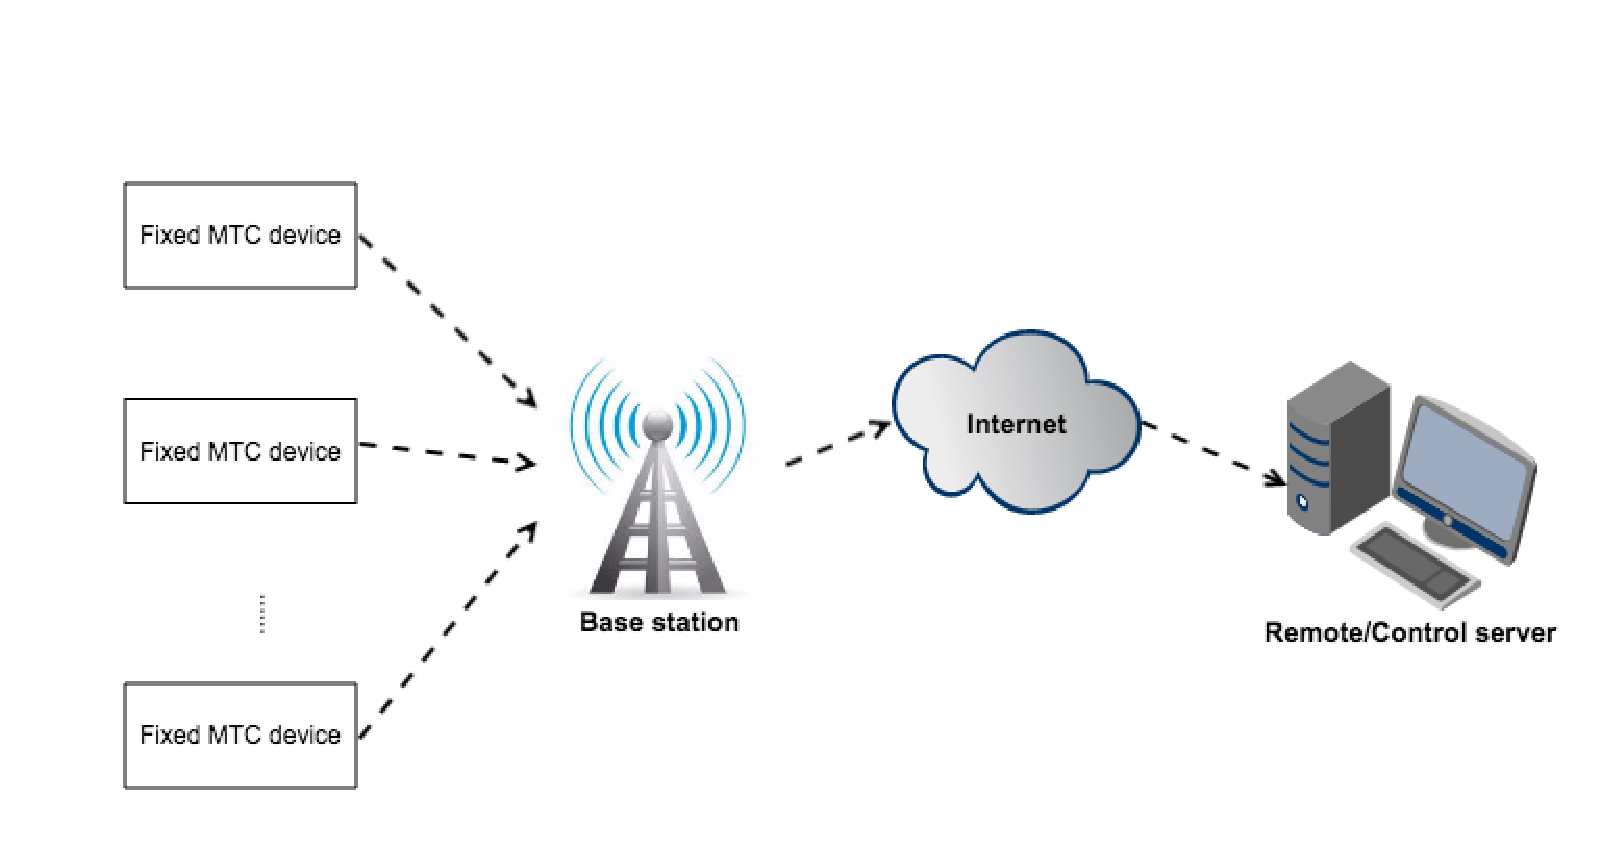
\includegraphics[width=\linewidth]{Chapter6/Figures/Time-driven-work-flow.eps}
	\caption{Periodic M2M application  work flow}
	\label{fig:Time-driven M2M work flow}
\end{figure}
Deployed in current LTE network, to finish data transmission, a device should repetitively go through three procedures: contention-based random access procedure for establishment of RRC connection, data transmission and release of established RRC connection. Note that term device and UE are used interchangeably in the rest of this chapter.
\subsection{Random access procedure}
\begin{figure*}[!t]
	\centering
	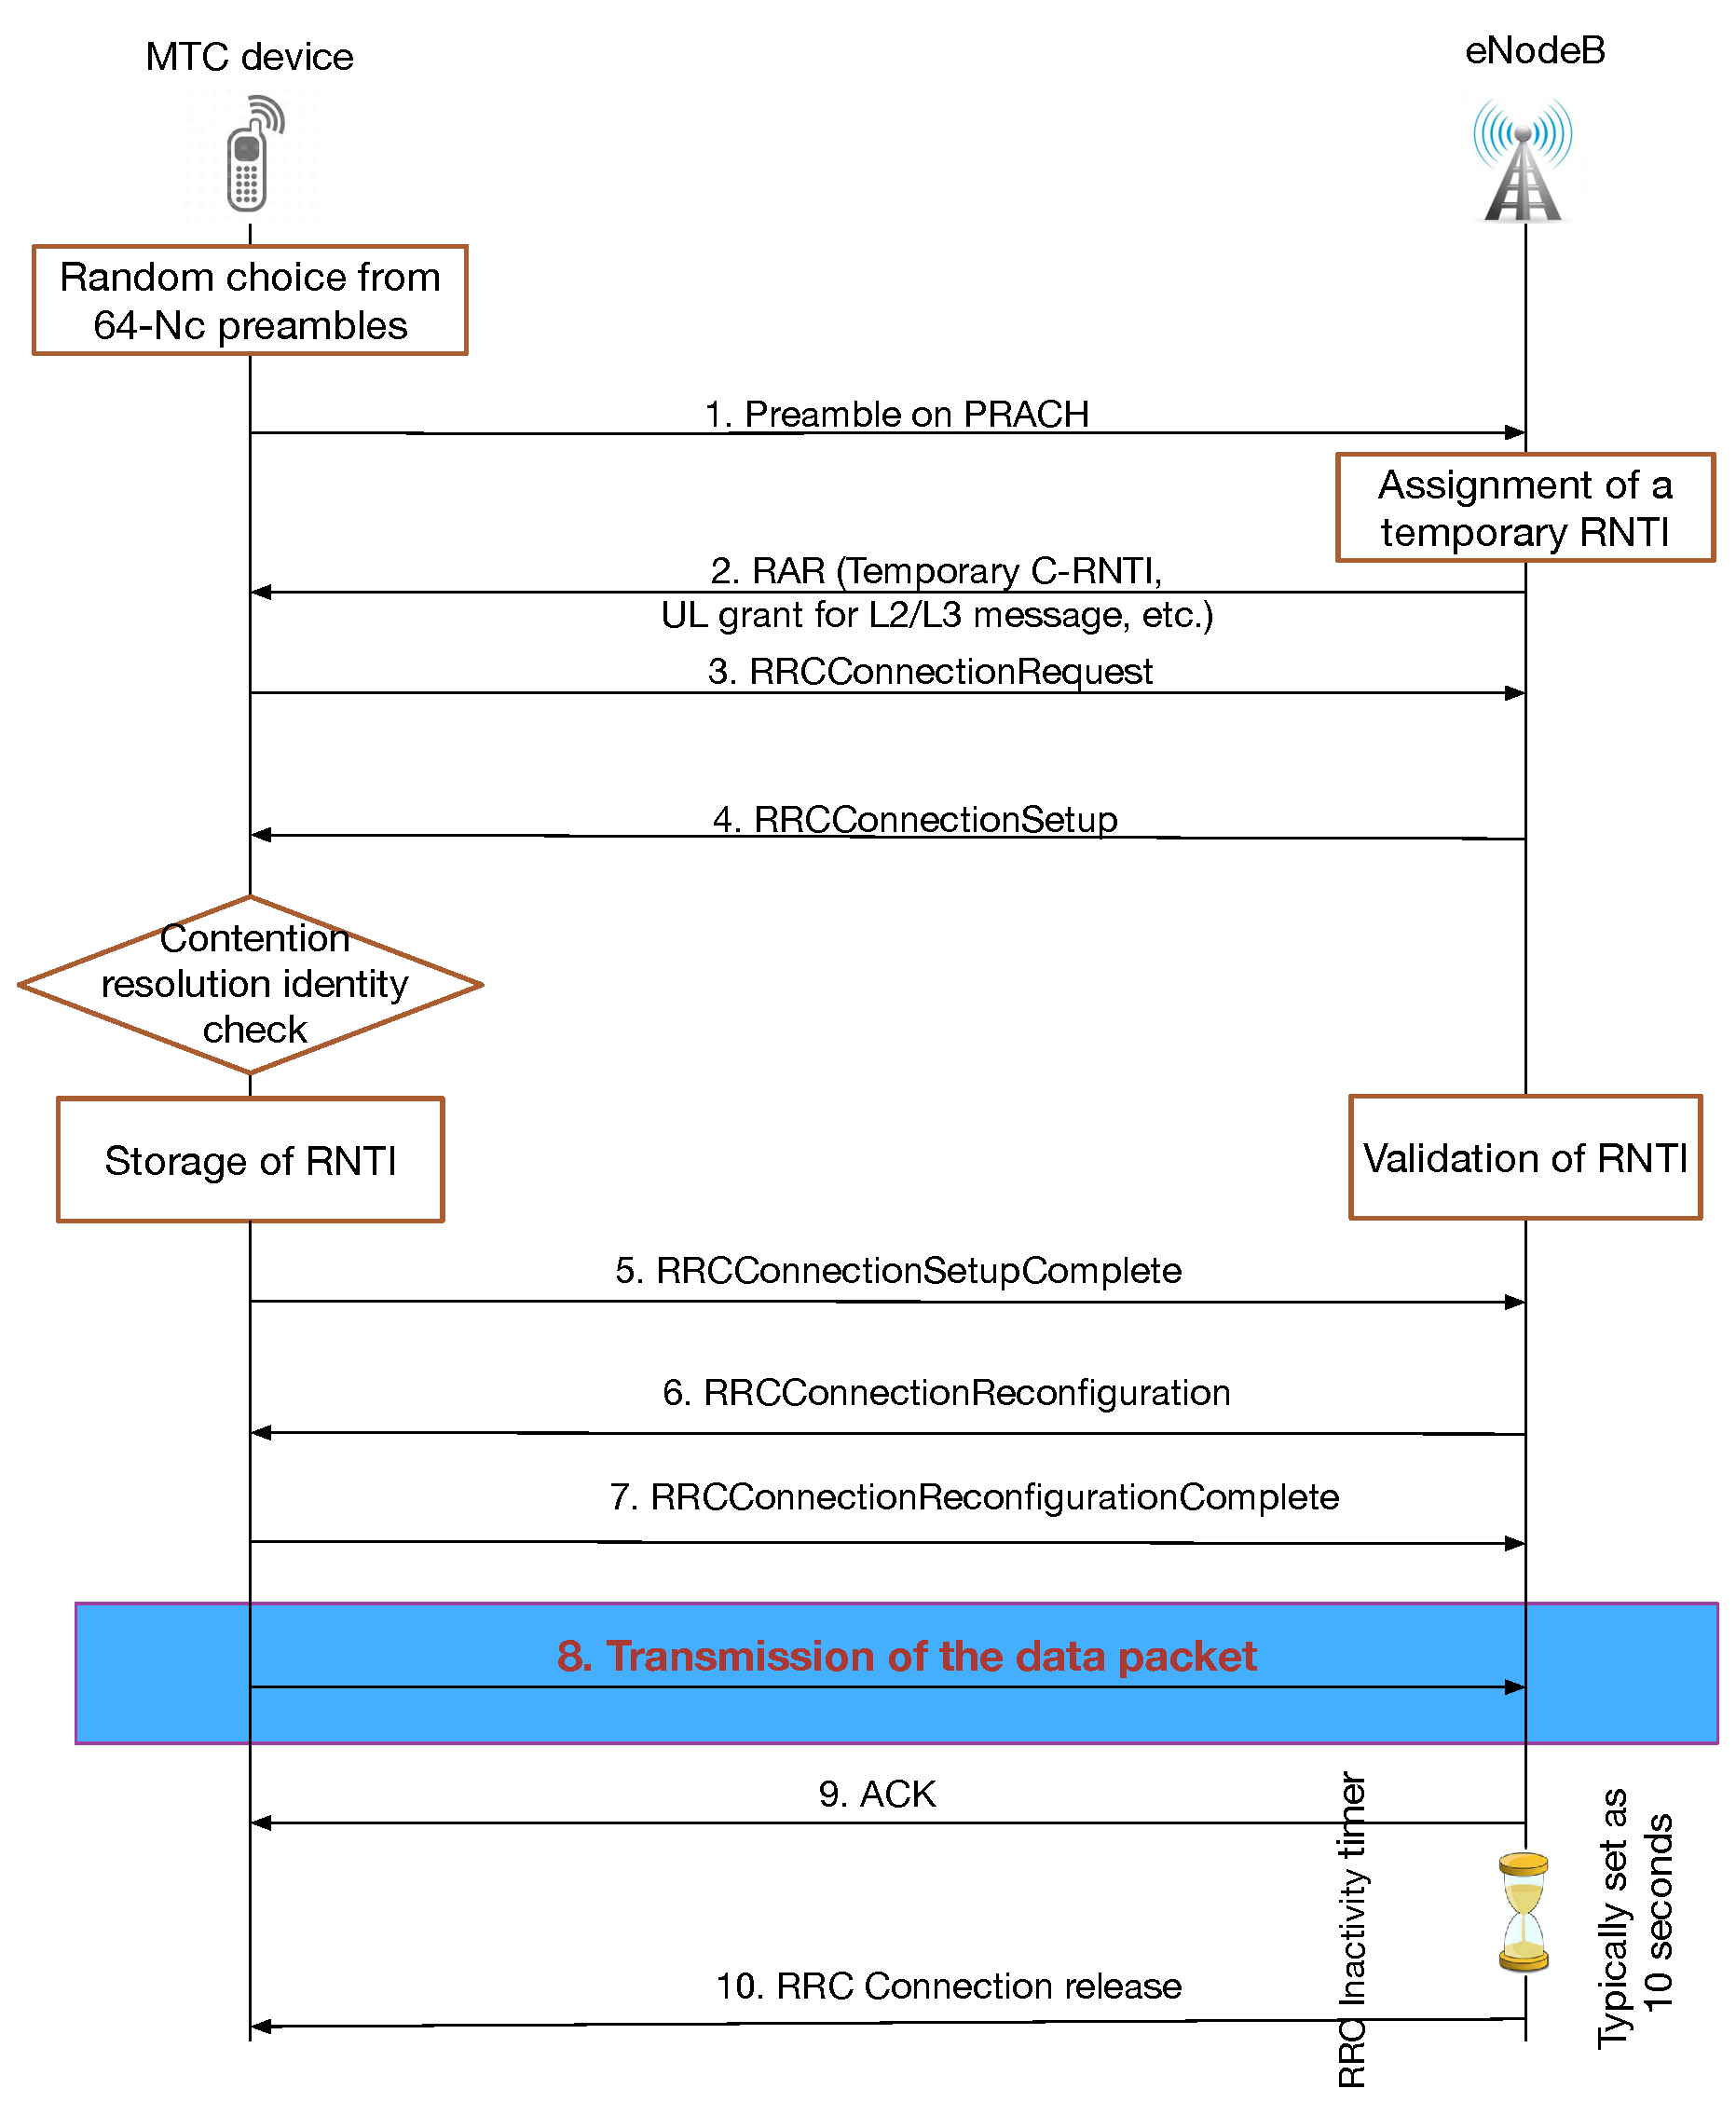
\includegraphics[width=\linewidth]{Chapter6/Figures/lte-ra.eps}
	\caption{Random access and data upload procedure in LTE networks}
	\label{fig:lte-ra}
\end{figure*}
As illustrated in Fig.~\ref{fig:lte-ra}, the random access procedure mainly consists of four steps presented as following. 
% 拉格朗日对这部分的建议是,到第四步再写 collision的情况
\begin{description}[font=\normalfont]
	\item[Step 1: Preamble transmission]\hfil \\
	In this step, the UE randomly selects one from the $64-N_c$ random access preambles and transmits the selected preamble at the next physical random access channel (PRACH) opportunity, where $N_c$ is the number of preambles reserved for non-contention based random access. After the preamble transmission, the UE shall monitor the PDCCH channel and try to decode a Random Access Response identified by the RA-RNTI from the eNB. %Note that the method to construct RA-RNTI is the same for UEs and eNB:
	% 每一步的写作思路是,先描述entity (UE, eNB) 内部如果运作,最后向对方发送什么内容,以及发送后的行为
	% 参考内容:
	% weblink : http://nitintayal-lte-tutorials.blogspot.fr/2013/09/random-access-procedure-rach.html
	% The mail answered by Xavier
	% Book: LTE-The UMTS Long Term evolution, from theory to practice	
	\item[Step 2: Random Access Response (RAR) ]\hfill \\
	%	After receiving RACH request in step1, The eNB PHY (Physical layer) calculates the timing advance which is transmitted to the UE as part of response message. %http://nitintayal-lte-tutorials.blogspot.fr/2013/09/random-access-procedure-rach.html
	The RAR message generated by the eNB is decoded with UE-generated RA-RNTI and contains the identity of the detected preamble, uplink channel synchronization information, an initial uplink resource grant for the transmission of the step 3 message, an assignment of a temporary Cell Radio Network Temporary Identifier (C-RNTI) along with other information. 
	\item[Step 3: L2/L3 message] \hfill \\
	%MSG3 (RRC Connection Reqeust)
	In this step, the UE sends the messages related to RRC connection request for random access procedure and makes use of Hybrid Automatic Repeat reQuest (HARQ). It is addressed to the temporary C-RNTI allocated in RAR at step 2 and carries the contention resolution identity. The contention resolution identity is a locally unique identity of the UE, which is generally built with the S-TMSI. After the transmission of step 3, the UE wait for the contention resolution message.
	\item[Step 4: Contention Resolution Reception] \hfill \\
	The contention resolution message from the eNB is addressed to the temporary C-RNTI and contains contention resolution identity received in L2/L3 message. This is an echo mechanism: if the UE detects its own identity, it knows that its random access request is accepted by eNB. If not, UE can infer that collision happens in previous step. A collision is occurred if more than one UEs select and send the same preamble to eNB in step 1. Each of them receives the same RAR in step 2 and thus uses the same same temporary C-RNTI in step 3. Either none of devices receives contention solution message and all colliding UEs restart from step 1, or just one of them receives echo and finishes the random access procedure.
\end{description}


\subsection{Transmission of data packet}
Since upload of MTC device data consists of a UE triggered service request procedure, L2/L3 message in previous is actually a RRCConnectionRequest and Contention resolution message is RRCConnectionSetup. Subsequently the UE sends service request in message RRCConnectionSetupComplete. After an exchange of RRCConnectionReconfiguration, UE establishes a RRCConnection network and starts the data transmission.
% http://lteuniversity.com/get_trained/expert_opinion1/b/lauroortigoza/archive/2013/12/18/rrc-connection-release.aspx
% 参考这一部分
\subsection{RRC Connection Release}
After transmission of data packet, UE goes back to RRC\_Idle state after the expiration of RRC inactivity timer, eNB deletes complete UE context and releases the established RRC connection with UE. Thus, UE has to pass through above steps before getting a RNTI for the next reporting.

With above description, traditional RACH access method poses some challenges when handling MTC in particular periodic MTC traffic. First massive device requests may lead to access network congestion. Second the control signaling overhead for small payload (e.g. $100$ bytes) is expensive, for example acquiring radio access network resources requires at least four messages exchanged between devices and network. Third short transaction for small payload causes inefficient resource utilization. Taking the consumption of RNTI as an example: assuming a MTC device needs to send $100$ bytes to remote server,  with a robust modulation scheme, the transmission is usually finished in $100$ ms, MTC device does not need to hold allocated RNTI until next reporting. However, the eNB has no way to determine whether device has data to transmit and takes back allocated RNTI after the expiration of related timer. 
%In addition, if periodic M2M application recoveries from a power outage, all managed MTC devices simultaneously try to connect eNB, which leads to a high collision level in radio access network. 
%Therefore, current RACH leads to waste of system resource and high overhead for each transmission if directly applied for MTC.
% 修改这部分标题,Xavier的意思是 这是直接在reseau de transport中提供的一种service 所以

\section{Network integrated M2M-oriental polling service}
\label{sec:polling}
The main idea of our proposed service is: the network provides a list of polling periods. MTC devices register to network for an appropriate polling period by traditional random access procedure. 
% 拉格朗日说,这句话英语表述有问题 C'est pas claire, il y un problème englais,surtout tu suppose qu'on va allouer les ressources
Upon received requests, the eNB deterministically allocates RNTI and the phase number in the allocated polling period for each registered device.
% according to proposed algorithm (detailed in Sec.\ref{prposed_algorithm}). This coordination mechanism schedules all data transmissions without collision.
% Ce que nous allouons est justement le RNTI, mais ensuite, il n'y a pas d'allocation fixe. Donc je suggère de dire: il y a en fait deux modes, c'est à dire, on peut avoir semi-static allocation (on peut avoir une allocation vraiement de type circuit); ou alors on peut avoir flexible packet access  (flexible allocation): 
% 'There are two possible modes: the first is the semi-persistent allocation where a fixed resource is periodically allocated to a MTC device. ' The second possibity is flexible allocation, where the standard packet access is used by a window defined for this polling period a MTC device pass standard packet access  
Afterwards, both the eNB and devices monitor LTE frames to determine their respective actions. When a transmission condition is verified for a certain device, the eNB directly allocates radio resources for the latter to poll the data. The qualified device directly sends its data via allocated resource without collision with other devices. Note that the radio resource allocation for data transmission may be of two types: either a semi-persistent allocation by which a fixed resource is periodically allocated to the registered MTC devices, or a flexible allocation where a standard packet access is used within the allocated polling window (detailed in Sec.\ref{polling-window}). 
%For radio resource allocation when transmitting data, there exist two possibilities: one is semi-persistent allocation 
Therefore, our proposed service consists of periodic polling mechanism and RNTI allocation algorithm. 
In this section, we first introduce some important concepts for our proposal. Second, we detail the periodic polling mechanism. Third, we present the RNTI allocation algorithm. 
\subsection{Definition}
% il faut aborder le fait qu'il y une correspondance entre PRD-RNTI et IMSI en fonction du temps... 
% Ce que nous allouons a mobile est une periode(polling period) et PRD-RNTI..
% 那拉格朗日的意思应该是 我们把polling period paging和给他分配的PRD-RNTI告诉手机啊。。。“Tu(un mobile) as telle period et telle PRD-RNTI quand le extened SFN modulo une variable. Il faut aussi preciser cette valeur...  Cela est indique par le reseau...”

% Quand un mobile se presente, il va demander une period. On va dire, OK, tu as telle periode et telle PRD-RNTI a tels moments. C'est quand le eSFN modulo une valeur 

%?“Comment le mobile sais quand il a ce PRD-RNTI???”
\subsubsection{LSFN}
\label{LSFN}
We propose to extend the frame counting mechanism of LTE known as SFN (System Frame Number) and define a counter called LSFN for Long SFN. It is used to help\begin{inparaenum}[i)]
	\item the eNB to determine which target it should poll for data 
	\item a device to determine whether it is its turn to transmit data.
\end{inparaenum}
 The necessity for this extension is due to the fact that conventional LTE SFN varies from $0$ to $1023$ and each SFN value repeats every $10.24$ sec. LSFN is constructed by extending $19$ bits as MSB (Most significant bit) for current SFN. The value of LSFN is reset when it reaches 14$\times$16875 $\times$1024. The period is thus 14$\times$16875$\times$1024$\times$10 ms, which is exactly $28$ days and allows to define any process with period up to about one month.
The 19 MSB of LSFN is broadcasted in a System Information Block every $10.24$ sec. 
The relationship between LSFN and SFN is shown in Fig.\ref{fig:construction of LSFN}.  
Note that the LSFN indexing system does not modify the SFN-based mechanisms. 
Terminals other than those of periodic MTC applications still access network through conventional random access and use current LTE SFN system. 

\begin{figure}[!t]
	\centering
	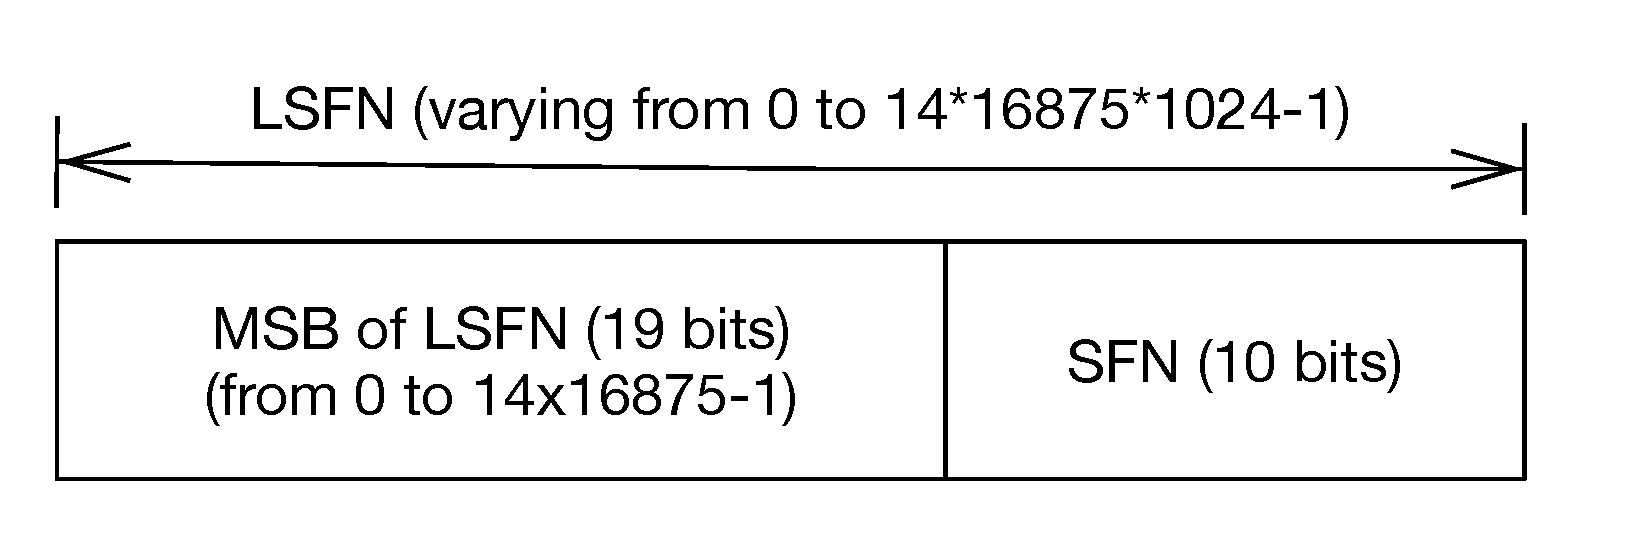
\includegraphics[width=0.6\linewidth]{Chapter6/Figures/Construction-LSFN.eps}
	\caption{Construction of LSFN}
	\label{fig:construction of LSFN}
\end{figure}

\subsubsection{PRD-RNTI}
\label{PRD-RNTI}
PRD-RNTI is a kind of RNTI used to uniquely identify one MTC device in a polling window (detailed in \ref{polling-window}).
The range FFF4-FFFC (marked as reserved for future use in \cite{3GPP/TS/36321}) is thus allocated as PRD-RNTI. 
%PRD-RNTI is reserved to a certain MTC device at the beginning of each polling window and released at the end of the same polling window then reallocated to the next polled MTC device. Network keeps a mapping table between PRD-RNTI and devices identity to consult which MTC device keeps which PRD-RNTI at a given moment. one PRD-RNTI can sequentially serve enormous MTC devices.
The same PRD-RNTI is allocated to several MTC devices but at different time. Hence, during a given period of time, the PRD-RNTI is allocated to only one device. As the allocation is deterministic, one device knows when it can use the PRD-RNTI and the network knows to which device the PRD-RNTI is used at any time. One PRD-RNTI can sequentially serve enormous MTC devices.

\subsubsection{{Polling period}}
\label{polling-period}
% 关于Polling period的notation是使用T_n还是T_p,n 让人伤脑筋啊
The polling period denoted by $T_n$ is the time interval between two consecutive eNB-triggered polling procedures for the same MTC device. It is computed from the application report period $T$ by:
\begin{align}
T_{n} = 2^{\floor{\log_2 \frac{T}{WT_f}}}\cdot W \cdot T_f =N_{n}\cdot W \cdot T_f\label{eq:period-conversion}
\end{align}
where $\floor{x}$ means the maximum integer not greater than $x$, $N_{n}$ is the number of polling window contained in period $T_{n}$, $W$ is the number of LTE frame, $T_{f}$ refers to LTE frame duration. As a network integrated service, the eNB uniquely supports polling periods satisfying (\ref{eq:period-conversion}). 
%Each user defined report period should be converted to an approximate polling period to use this network-integrated service. For example, a report period $300 s$ is converted to $204.8s$ as polling period.

% sur une period ou bien une interval du temps, il y a une correspondance entre mobile et RNTI

\subsubsection{{Polling period}}
\label{polling-period}
% 关于Polling period的notation是使用T_n还是T_p,n 让人伤脑筋啊
The polling period denoted by $T_n$ is the time interval between two consecutive eNB-triggered polling procedures for the same MTC device. It can be represented by the combination of three primes $2,3,5$. Namely, $T_n =  2^{a} \cdot 3^{b} \cdot 5^{c}$, where $a, b, c$ are the occurrence number of the corresponding prime. For a given $T$, we choose the closet $T_n$ to use polling service.
\begin{align}
T_{n} = 2^{a} \cdot 3^{b} \cdot 5^{c}\cdot W \cdot T_f\label{eq:period-conversion}
\end{align}
where $\floor{x}$ means the maximum integer not greater than $x$, $N_{n}$ is the number of polling window contained in period $T_{n}$, $W$ is the number of LTE frame, $T_{f}$ refers to LTE frame duration. As a network integrated service, the eNB uniquely supports polling periods satisfying (\ref{eq:period-conversion}). 
%Each user defined report period should be converted to an approximate polling period to use this network-integrated service. For example, a report period $300 s$ is converted to $204.8s$ as polling period.

% sur une period ou bien une interval du temps, il y a une correspondance entre mobile et RNTI

\subsubsection{Polling window}
\label{polling-window}
The polling window is a time interval which is reserved for data transmission of a unique MTC device. It is a configurable system parameter. Its duration is equal to $W$ LTE frame and should ensure that the device can deliver its data even in case of retransmission due to the HARQ mechanism.
The relationship between polling window and LTE frame is illustrated in Fig.\ref{fig:Illustration of Polling window in time domain}. 

\begin{figure}[!t]
	\centering
	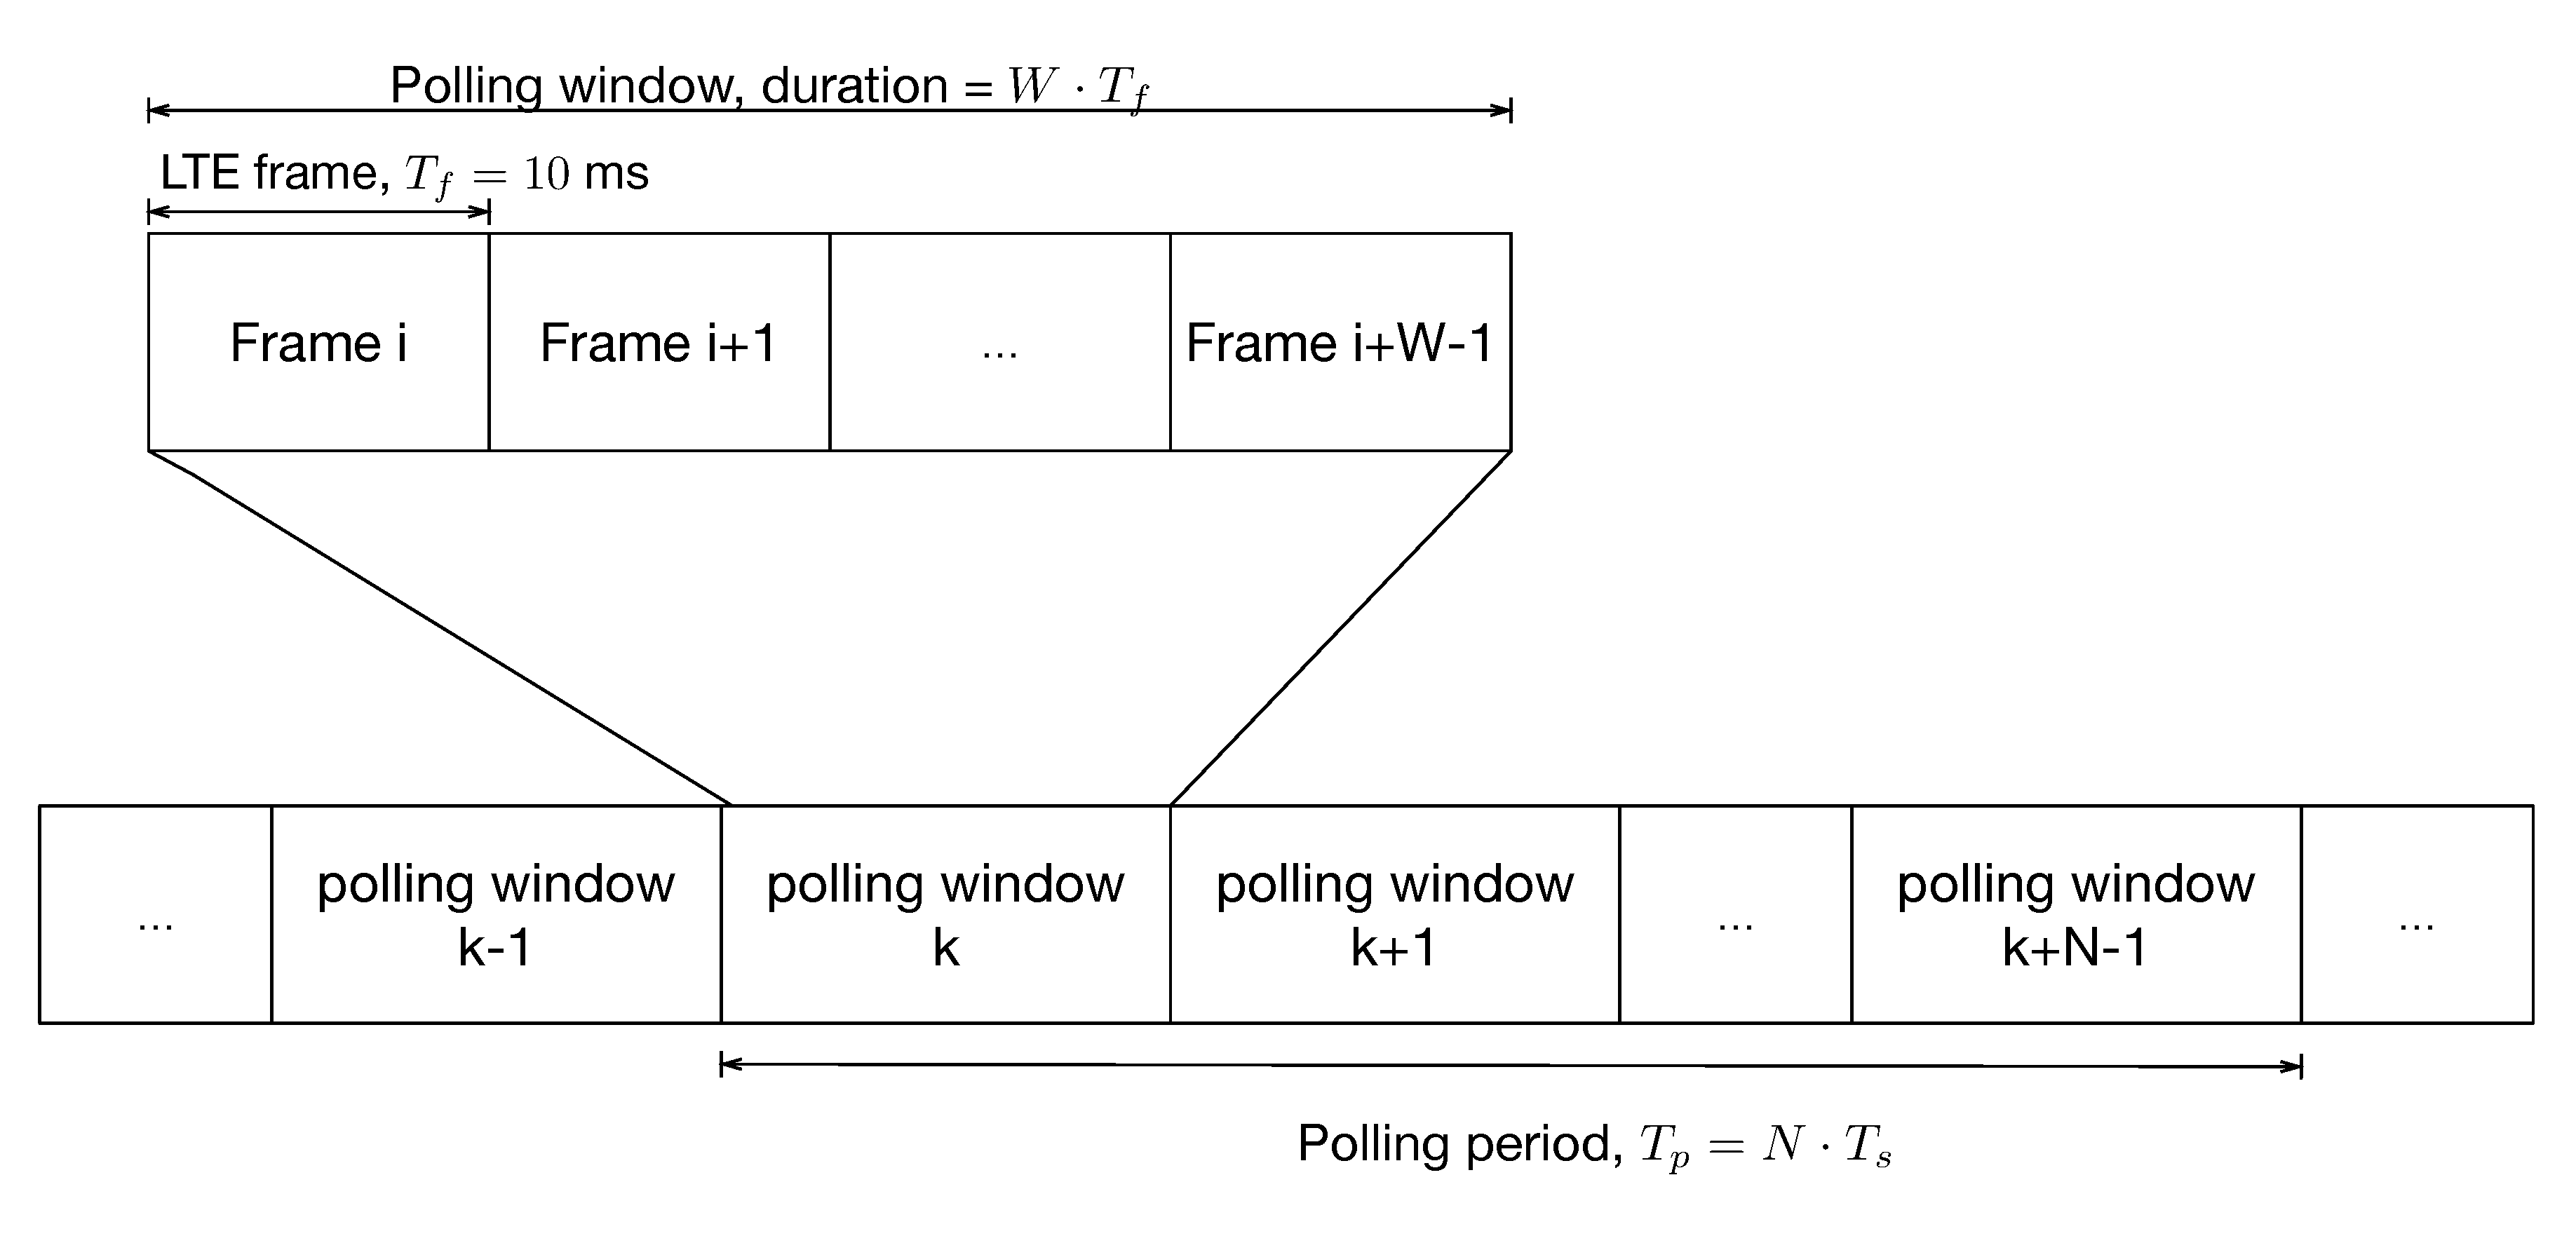
\includegraphics[width=0.9\linewidth]{Chapter6/Figures/Polling_window_illustration.eps}
	\caption{Illustration of Polling window in time domain}
	\label{fig:Illustration of Polling window in time domain}
\end{figure}

% 接下来讨论 polling window的长度 
%Supposing the maximum retransmission number is set as $3$, the worst case is that eNB receives report from device after four times transmission and takes in total 32 ms if each transmission takes $8$ ms. This analysis procedure is illustrated in 
%%8 ms for a transmission comes from where??
%in Fig.\ref{fig:UE Transmission and 3 Retransmission}. If taking into account possible eNB response to MTC device, a conversation including a report and response can be achieved in $64$ ms. Thus, we define in our proposal the duration of polling window as $100$ ms ($10$ LTE frames).
%\begin{figure}[htbp]
%	\centering
%	\includegraphics[width=10cm, height= 8cm ]{Figures/UE-Retransmission.png}
%	\caption{UE Transmission and 3 Retransmission}
%	\label{fig:UE Transmission and 3 Retransmission}
%\end{figure}

% 关于mobile是如何知道自己是在什么时候可以上传数据的设想:
% 方案一: 用户在购买SIM卡的时候,什么时候报告,分配什么PRD-RNTI都已经确定好了 然后输入到eNB的数据库里。。
% 方案二: 用户的设备的安放到 某个eNB管理下的小区的时候, 自己像eNB发出特设的信息(这岂不是还是有点儿类似于RA么),然后eNB会为其分配 指定的 上报时机以及 PRD-RNTI
% 个人感觉,拉格朗日所言更像是 方案二
\subsection{Multiple-period polling mechanism}
%Simply speaking, periodic polling mechanism refers to allocate resource to a certain MTC device at a given time. Since periodic MTC applications comportment is deterministic, we could define a deterministic rule for resource allocation for each device.

Different with traditional RACH method for network access, the eNB in our proposed periodic polling mechanism allocates system resource (i.e. RNTI) to a certain registered MTC device when LSFN satisfies some predefined rules, since periodic MTC application comportment is deterministic. It consists of two stages: registration stage and polling stage. 

\subsubsection{Registration stage} 
%在这个问题上,貌似拉格朗日跟我有分歧啊。。。
%我的想法是,device只是上报用户设置的 reporting period,由eNB负责conversion然后把确定好的 polling period下行给 device.
Let consider one MTC device $m$ asking for periodic polling service. It first sends a polling activation request including the polling period $T_n$ by traditional random access procedure. If the request is accepted, the network then sends back a confirmation message with \begin{inparaenum}[i)]
	\item the number of polling windows $N_n$ that corresponds to the polling period;
	\item a phase value $\phi _{m}$ between $0$ and $N_{n}-1$;
	\item a PRD-RNTI value.
\end{inparaenum}
Once the registration stage is finished, eNB updates its internal data for periodic polling service and registered device $m$ can use allocated PRD-RNTI with following rules: 
\begin{align}
&\textrm{PRD-RNTI for device $m$} \textrm{ when} \floor{\frac{LSFN}{W}}\bmod N_n=\phi _{m} \label{eq:rule}
\end{align}
%where $\floor{\frac{LSFN}{W}}$ means the maximum integer not great than $\frac{LSFN}{W}$.
\subsubsection{Periodic polling stage}
At this stage, for each LTE frame, the eNB manipulates LSFN value and determines current polling window is reserved for which MTC device by checking stored rules like in (\ref{eq:rule}). Still taking device $m$ as an example, once rule (\ref{eq:rule}) is satisfied, the eNB allocates radio resource for the device holding the PRD-RNTI, namely device $m$. As to device $m$, it also monitors the value of LSFN. If the MTC device has no specific action, it can switch to a low consumption mode in order to spare energy. As soon as rule (\ref{eq:rule}) is checked then the device $m$ listens to the PDCCH during all the polling window. It is up to the eNB to allocate uplink radio resource in order to allow the data transmission of the MTC device. Note that the PRD-RNTI is allocated to only one device during a given polling window. Standard system resource allocation mechanisms can be used without any risk of collision. This procedure is illustrated in the right part of Fig. \ref{fig:Comparison}.

Finally, Fig.\ref{fig:Comparison} illustrates the comparison between MTC device data report via conventional random access and our proposal.
%: In RACH mechanism, MTC device has to pass three transmission for reporting collected data while in our proposal it needs just one transmission.
%Unlike traditional random access method, for a already registered MTC device, it manipulates the $LSFN$ received in System Information. When the condition for its turn of transmission, it directly sends collected data with received PRD-RNTI in PDCCH channel without demanding resource allocation.

\begin{figure*}[!t]
	\centering
	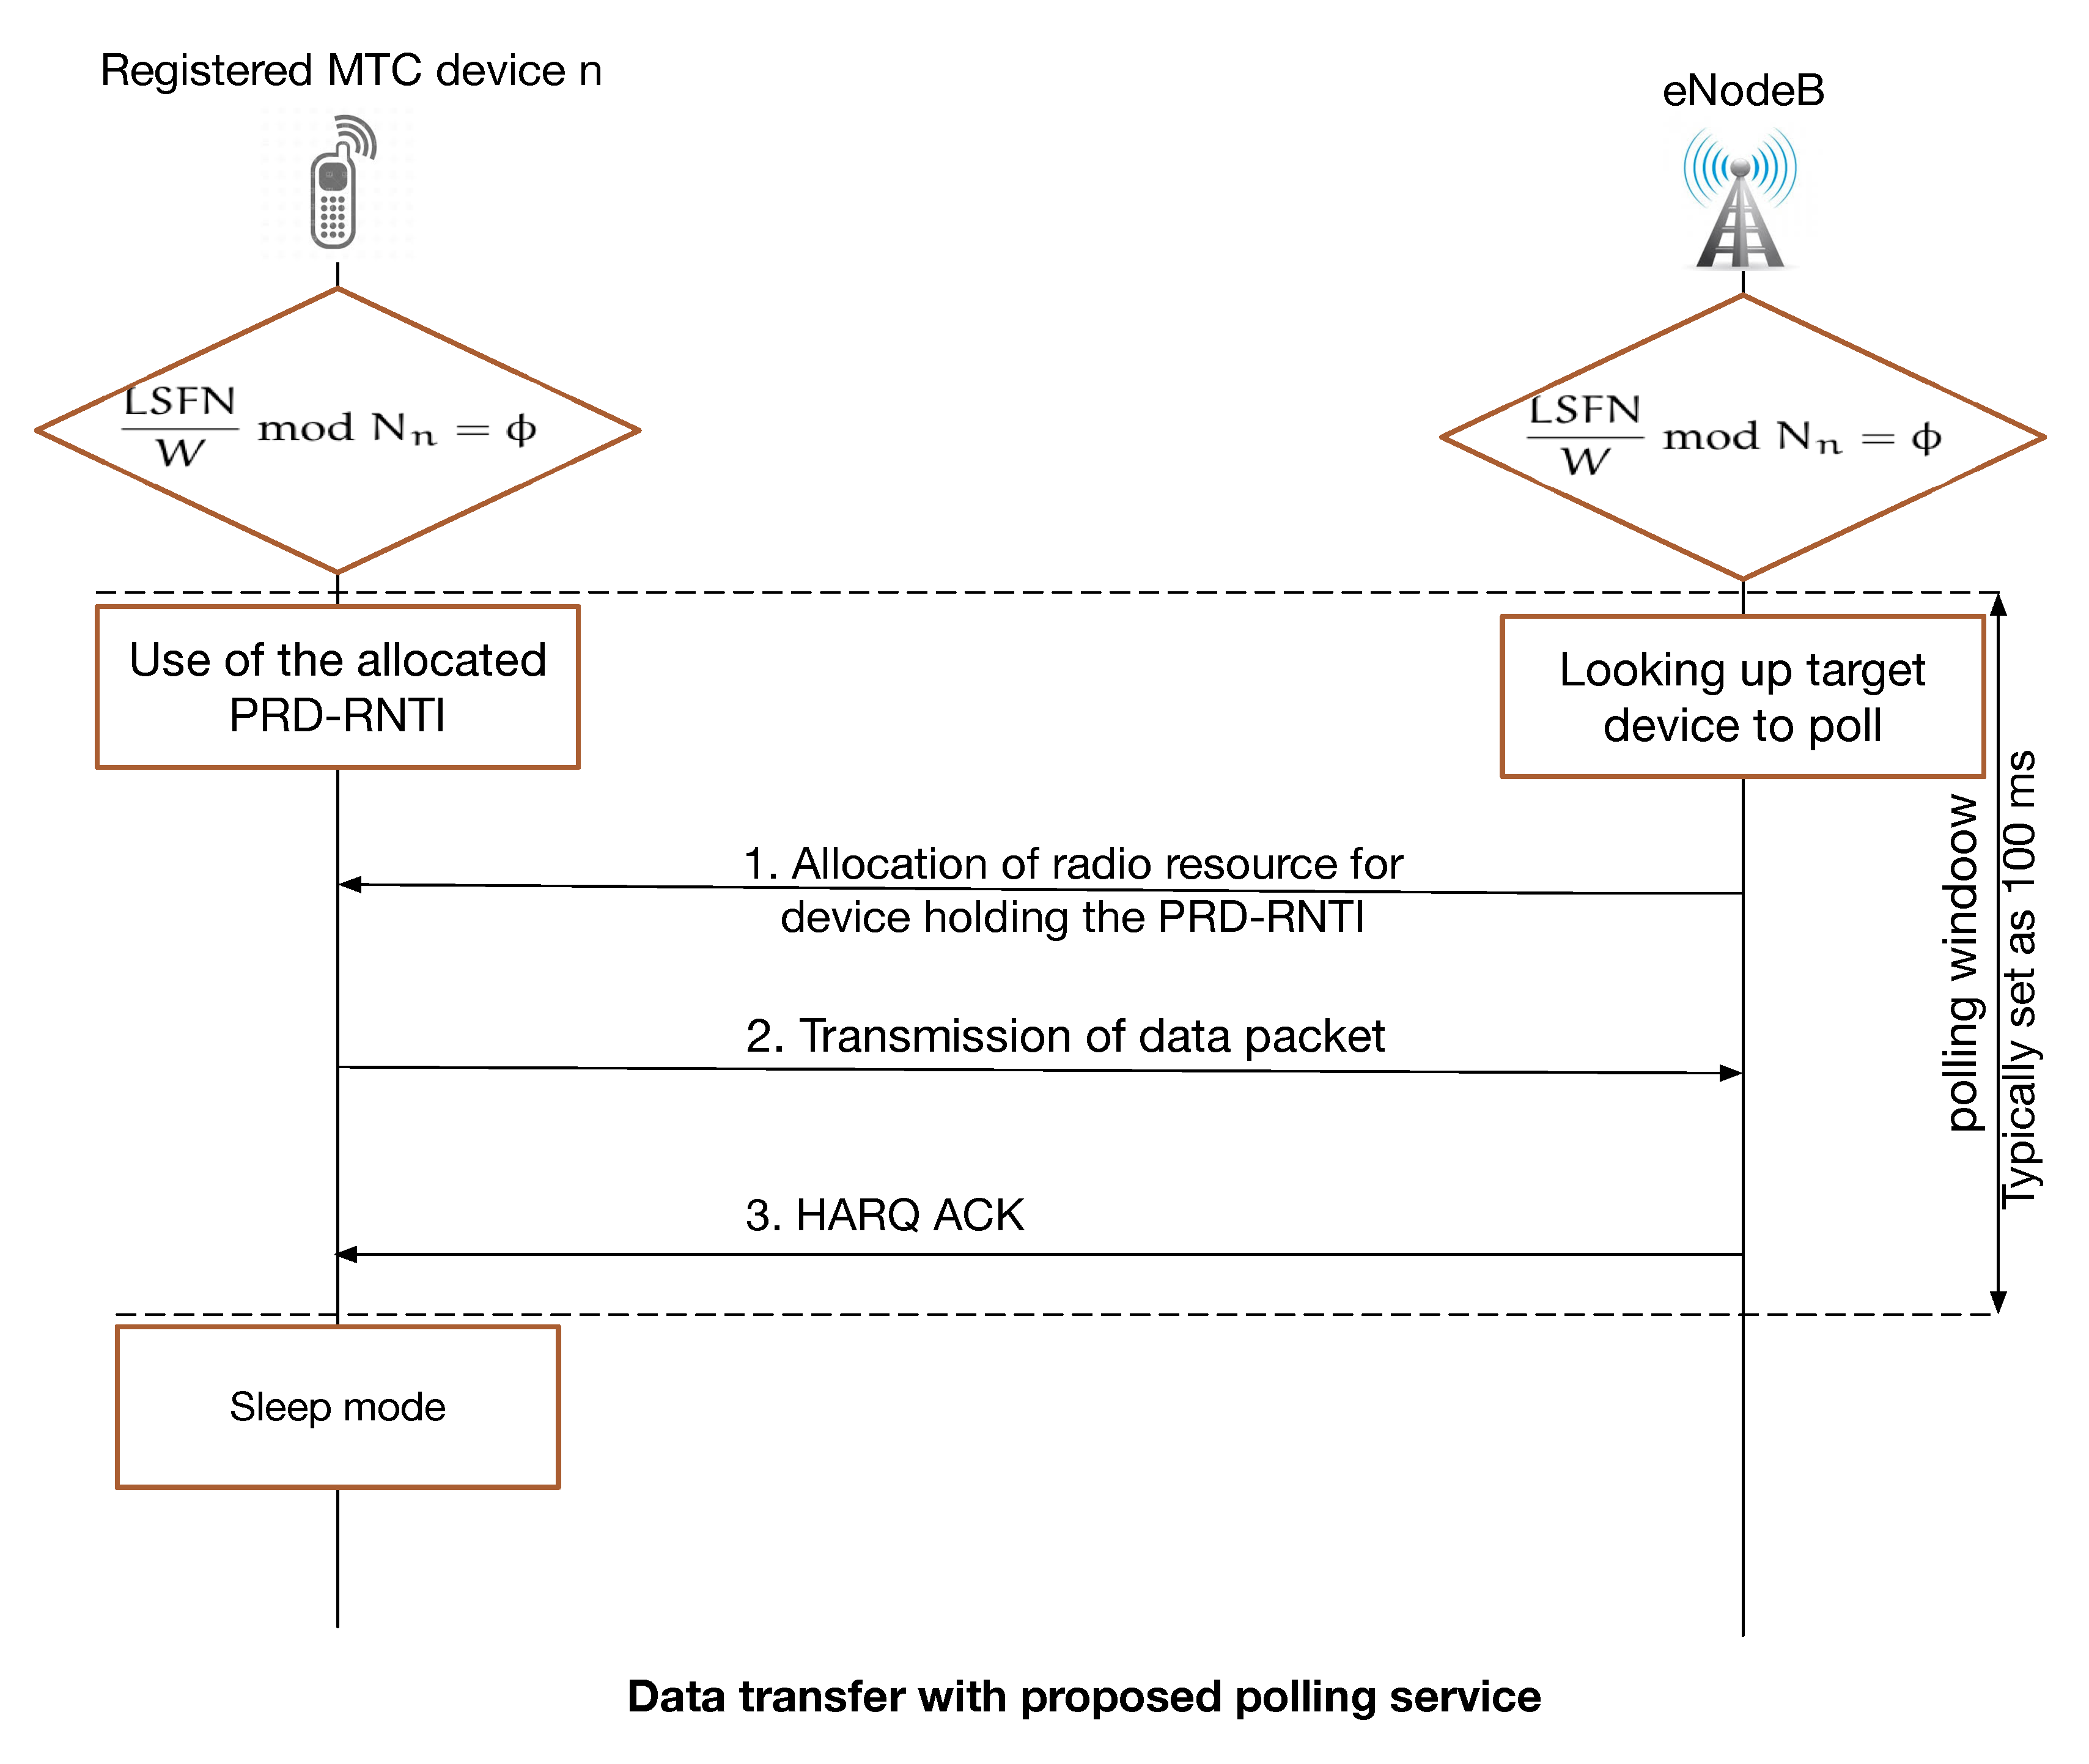
\includegraphics[width=\linewidth]{Chapter6/Figures/proposed-polling-service}
	\caption{Proposed polling service work flow}
	\label{fig:Comparison}
\end{figure*}
\subsection{RNTI allocation algorithm}
\label{prposed_algorithm}
%As introduced in previous section, time domain resource is divided into a series of polling windows and eNB supports a group of polling periods. A resource allocation algorithm \ref{alg:resource-allocation-algo} is thus proposed to allocate polling windows for each registered MTC device. A detailed explanation about this algorithm is given in this section.

%When receiving all requests, our proposed resource allocation algorithm \ref{alg:resource-allocation-algo} is executed for allocating polling window, for each registered device. 
Algorithm (\ref{alg:resource-allocation-algo}) serves for allocating resource such as PRD-RNTI and phase value 
(refers to a series of polling windows) 
for each registered device.
Some notations about our algorithm: the eNB provides $N$ different polling periods denoted by $T_{n}$, where $n=0,1,...,N-1$ and $T_{n} = 2T_{n-1}$. The number of polling windows in polling period $T_{n}$ is denoted by $N_{n}$. All devices are regrouped into $N$ groups according to polling periods with ascending order. The number of devices waiting for polling window allocation in group $n$ is denoted by $g_{n}$. Each PRD-RNTI provides a limited number of polling windows. The cardinality of available polling windows set when allocating for devices in group $i$ is denoted by $C_{PRD-RNTI, i}$. When there are no available polling windows, a new PRD-RNTI should be taken from PRD-RNTI set. 
The algorithm (\ref{alg:resource-allocation-algo}) first takes an available PRD-RNTI and initiates $C_{PRD-RNTI, 0}$ as $N_{0}$. A loop structure from line \ref{algo: for-loop-all-groups} to \ref{algo: end-for-loop-all-groups} is used to process all requests on the basis of group. In iteration $i$ for phase value allocation of group $i$, algorithm first calculates available polling windows $C_{PRD-RNTI, i}$ by a recursive relation $C_{PRD-RNTI, i}=2C_{PRD-RNTI, i-1}$, since the number of polling window contained in a polling period $N_{i} = 2N_{i-1}$. If the number of devices remaining to be processed is still more than $0$, algorithm enters in while-loop (line \ref{algo:while-loop} to \ref{algo:end-while-loop}) for allocating each device a polling window. In this while-loop, first check if it needs take a new PRD-RNTI. Then algorithm calculates allocated phase value $\phi$ for $\min (g_{i}, C_{PRD-RNTI, i})$ devices then updates $C_{PRD-RNTI, i}$ and $g_{i}$. 
%The condition to exit this while-loop is satisfied when there is no devices in group $i$ to be allocated polling window.
\begin{algorithm}
	\caption{RNTI allocation algorithm} % Title of this algo
	\label{alg:resource-allocation-algo} % Facilitate reference for this algo
	\begin{algorithmic}[1] % 1 --> show lines number
		\Procedure{Allocation}{$g_{0}, g_{1}, g_{2}, ..., g_{N}$} 
		\State $PRD-RNTI \gets $ $pop$ $PRD-RNTI$ $set$
		\State $C_{PRD-RNTI, 0} \gets N_{0} $
		\For{$i=0$; $i<N$; $i++$ } \label{algo: for-loop-all-groups}
		\If {$i > 0$}
		\State $C_{PRD-RNTI, i} \gets 2C_{PRD-RNTI, i-1}$
		\EndIf
		\While{$g_{i} > 0 $} \label{algo:while-loop}
		\If {$C_{PRD-RNTI, i} = 0$}
		\State $PRD-RNTI \gets $ $pop$ $PRD-RNTI$ $set$
		\EndIf
		\For{$j=0$; $j<min(g_{i}, C_{PRD-RNTI, i})$; $j++$ } \label{algo:allocation-for-loop}
		\State $\phi _{j} \gets \floor{\frac{LSFN}{W}} \mod N_{n} $
		\EndFor \label{algo:end-allocation-for-loop}
		\State $C_{PRD-RNTI, i} \gets C_{PRD-RNTI, i}-\min (g_{i}, C_{PRD-RNTI, i})$
		\State $g_{i} \gets g_{i} - \min (g_{i}, C_{PRD-RNTI, i})$
		\EndWhile \label{algo:end-while-loop}
		\EndFor \label{algo: end-for-loop-all-groups}
		\EndProcedure
	\end{algorithmic}
\end{algorithm}

\subsection{An example}
Let take an example to illustrate the proposed RNTI allocation algorithm. 
Supposing an eNB supports $4$ different polling periods whose notations are $T_0 = 4T_s, T_1=8T_s, T_2=16T_s, T_3=32T_s$, $T_s$ is duration of a polling window. All devices are regrouped into four groups $0, 1, 2, 3$. Each group consists of two devices so $g_{0}=2, g_{1}=2,g_{2}=2,g_{3}=2$ and each device is respectively identified as $a_{0}, a_{1}, b_{0}, b_{1}, c_{0}, c_{1}, d_{0}, d_{1}$. 
To allocate polling window for these devices, first take value $FFF4$ from PRD-RNTI set. For group $0$ with polling period $4T_s$, the available polling windows is $N_{0}=4$. Allocate respectively polling windows satisfying $\phi_{a_{0}}=0, \phi_{a_{1}}=1$ for $a_{0}, a_{1}$. Since there are just two devices to be served in group $0$, it still remains $2$ polling windows after allocation. Then for group $1$, at this time available polling window number is $4$ , allocate polling windows satisfying $\phi_{b_{0}}=2, \phi_{b_{1}}=3$ for $b_{0}, b_{1}$. So after allocation for group $1$, $C_{PRD-RNTI, i=1}$ is updated as $2$. With the same philosophy, allocation for group $2, 3$. The RNTI and phase value allocation result is shown in Fig.\ref{fig:Illustration-Resource-Allocation} and resumed in Tab.\ref{tab:resume}.
\begin{table}[!t]
	\renewcommand{\arraystretch}{1.3}
	\caption{Polling window allocation resume}
	\label{tab:resume}
	\centering
	\begin{tabular}{ccccc}
		\hline
		group name & number of device& identity & polling period & phase value \\
		\hline
		\multirow{2}{*}{0} & \multirow{2}{*}{2} & \multirow{2}{*}{$4T_{s}$} & $a_{0}$ & $0$\\ &&& $a_{1}$ & $1$ \\
		\hline
		\multirow{2}{*}{1} & \multirow{2}{*}{2} & \multirow{2}{*}{$8T_{s}$} & $b_{0}$ & $2$\\ &&& $b_{1}$ & $3$ \\
		\hline
		\multirow{2}{*}{2} & \multirow{2}{*}{2} & \multirow{2}{*}{$16T_{s}$} & $c_{0}$ & $6$\\ &&& $c_{1}$ & $7$ \\
		\hline
		\multirow{2}{*}{3} & \multirow{2}{*}{2} & \multirow{2}{*}{$32T_{s}$} & $d_{0}$ & $14$\\ &&& $d_{1}$ & $15$ \\
		\hline
	\end{tabular}
\end{table}

\begin{figure}[!t]
	\centering
	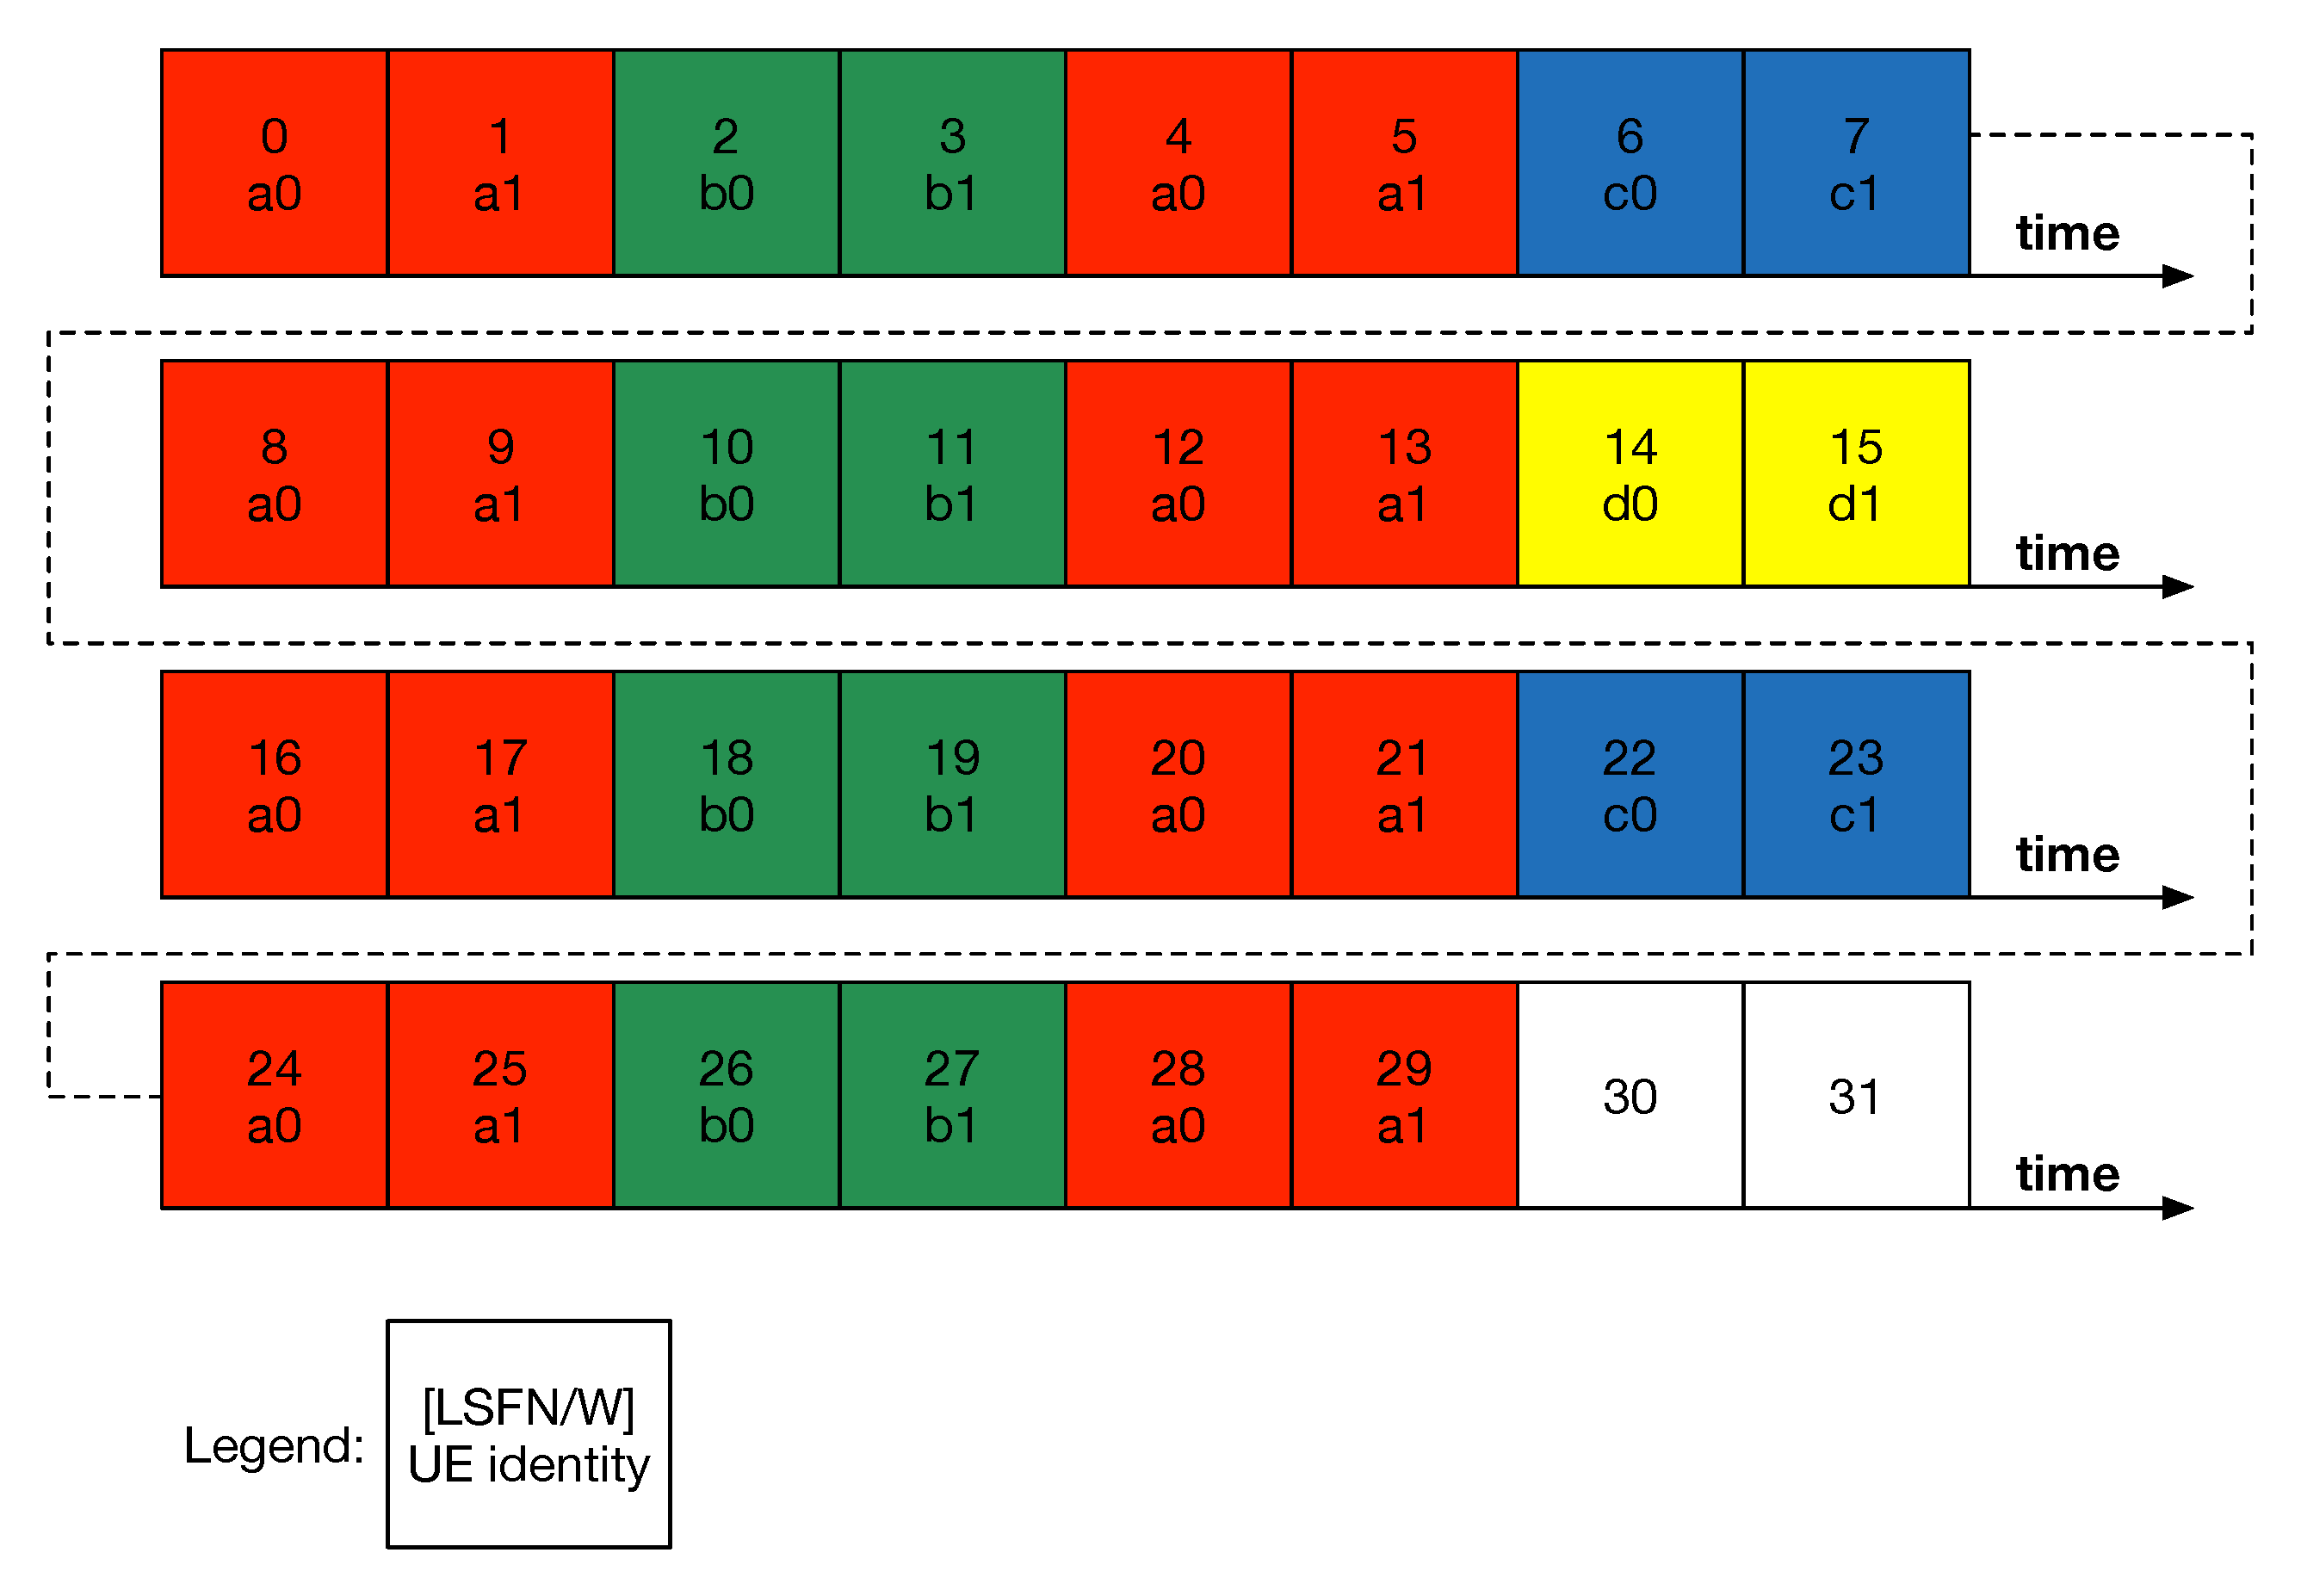
\includegraphics[width=\linewidth]{Chapter6/Figures/Anexampleallocation}
	\caption{Illustration of RNTI allocation result}
	\label{fig:Illustration-Resource-Allocation}
\end{figure}

\section{Performance Analysis}
\label{analysis}
% %TODO: is it better to consider a fixed length packet or variable length?
% %TODO: Whether this hypothesis should be kept? Radio link conditions are ideal and data reporting is finished in the first transmission. 
A comparative performance analysis between traditional RACH and our proposal (network integrated M2M-orientated polling service) is presented in this section. We focus on the consumption of RBs  (used for data transmission and signaling) and the minimum number of RNTI, for both methods.

\subsection{System model}
\begin{figure}[!t]
	\centering
	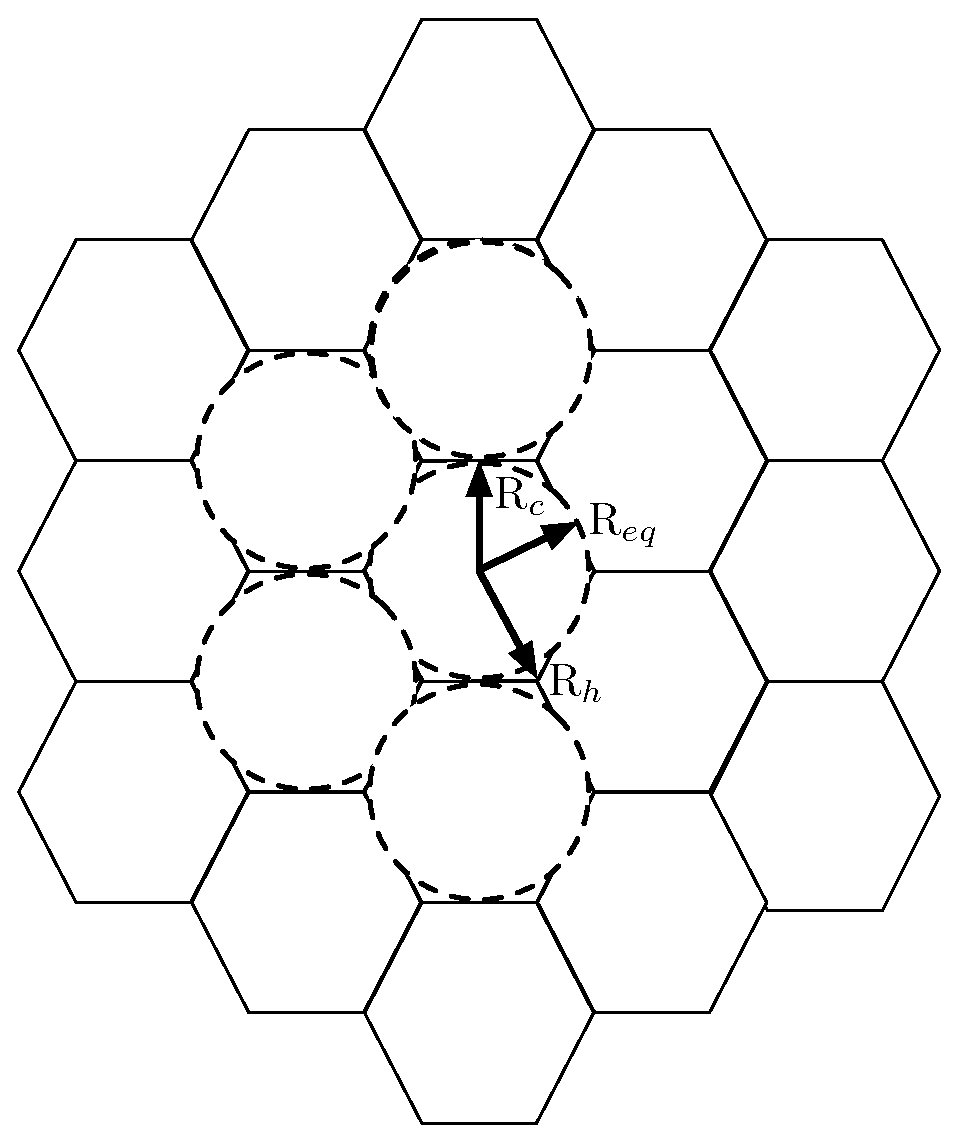
\includegraphics[scale=0.5]{Chapter6/Figures/hexagone_grid}
	\caption{The studied hexagonal grid network topology}
	\label{fig:hexagone_grid}
\end{figure}

We consider a regular hexagonal network whose topology is illustrated in Fig.~\ref{fig:hexagone_grid}, where $R_{h}$ refers to the hexagonal radius and $R_c$ denotes the half distance between two adjacent eNBs. We assume that all the eNBs have omnidirectional antenna so that each eNB covers a single cell. All eNB transmit with the same power.

The amount of MTC devices served by each eNB, denoted by $N_d$, is assumed to be very large. These devices are static and periodically sending data to remote servers. The device reporting period $T$ is assumed to be a random variable whose distribution can be of any type. To reduce the reporting collision rate, the report moment for each device is chosen uniformly between time interval $\left[ 0, T\right] $. 

Fractional power control is taken into account in this model. The path-loss is partially compensated by the power control scheme. The power compensation factor is denoted by $\alpha$. Okumura-Hata model~\cite{lagrange2000reseaux} is applied to model the propagation attenuation. Fading and shadowing are assumed to be averaged out. Thus, the received power at the receiver side can be expressed as follows: the path loss function $g(r)$ is:  
\begin{align}
P_r &= P_t \left( \frac{r_0}{r} \right) ^{\gamma(\alpha -1)} 
\end{align}
where $r$ is the distance between the receiver and the transmitter, $r_0$ is a constant determined by Okumura-Hata model and $\gamma$ is the path loss exponent. Note that all the eNB transmit with the same power without applying power control,  hence for downlink transmission, $\alpha = 0$. For uplink transmission, and $\alpha$ varies between $\left[ 0, 1\right]$.

In fact, performance analysis for a regular hexagonal grid network has no closed form expressions, however, such networks can be well approximated by the fluid model proposed in~\cite{kelif2010fluid} (circle in discontinuous lines in Fig.~\ref{fig:hexagone_grid}). The key idea of such a model consists in replacing a given fixed finite number of interfering sources by an equivalent continuum of transmitters. For example, when analyzing downlink interference, a limited area hexagonal network, which has a fixed number of eNB, now can be approximately replaced by a network with eNB density $\rho_{m}$.These eNBs are spatially uniformly distributed in the network. The eNB density $\rho_{m}$ is the ratio between the number of eNB and the network coverage area. 
%\begin{figure}[!t]
%	\centering
%	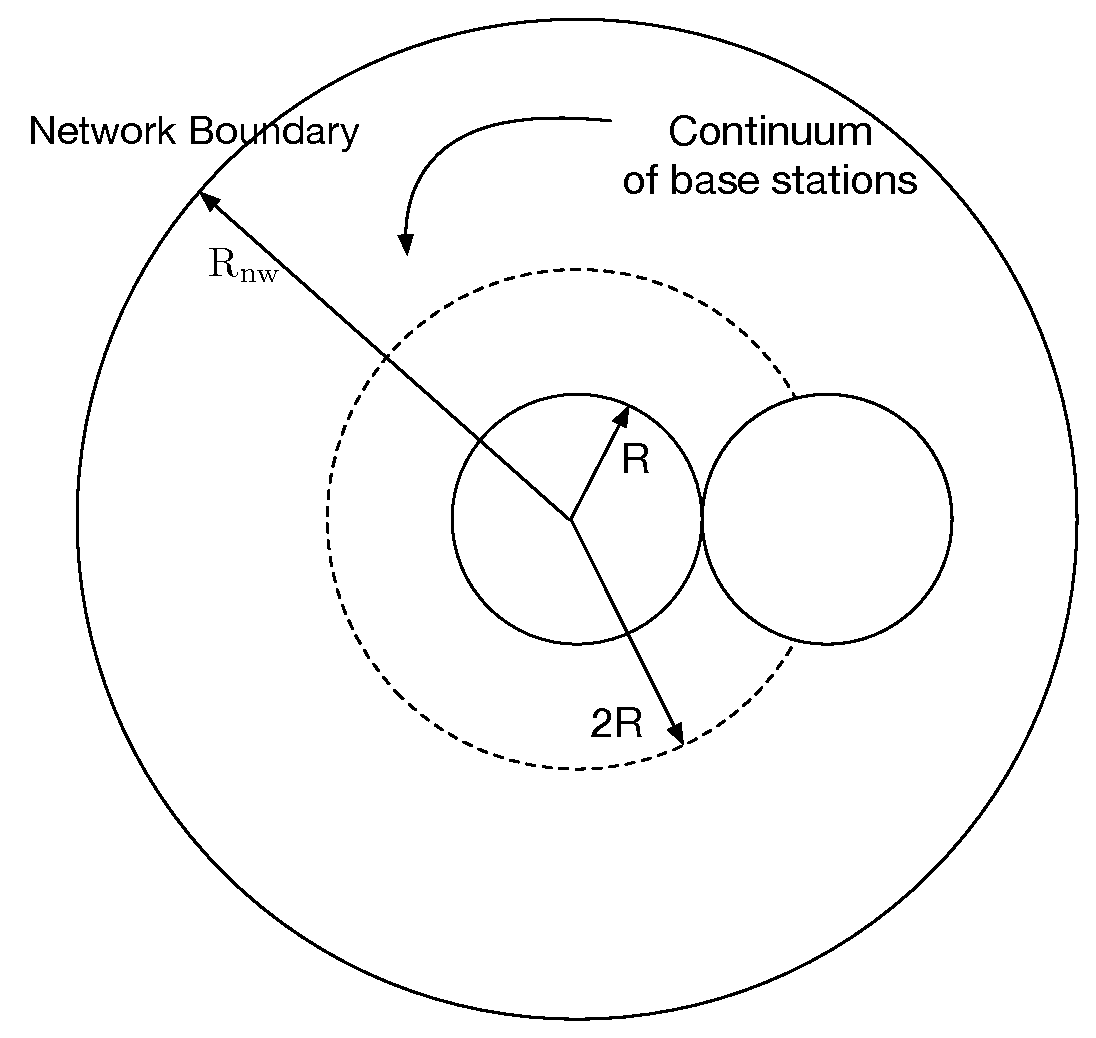
\includegraphics[width=0.7\linewidth, height=8cm]{Chapter6/Figures/fluid_model}
%	\caption{Fluid model illustration}
%	\label{fig:fluid_model}
%\end{figure}

\subsection{Lower bound of RNTI Consumption}
\label{sec:lower_bound_rnti}
Let $C_{\text{min}}$ be the low bound of RNTI required in the coverage zone of an eNB.

\subsubsection{Our proposal}
In a system with our proposed multiple period polling service, the utilization of RNTI is in a persistent manner. Hence, the number of occupied RNTI (i.e. PRD-RNTI) depends on the amount of device $N_d$ served by the eNB and polling period. 

Recall that eNB provides $M$ available polling periods. The polling period is denoted by $T_{n}$, where $T_n = 2^n \cdot W \cdot T_f$. The number of devices with the same polling period is denoted by $g_{n}$. For polling period $T_n$, there exist $2^n$ available polling windows. Thus with $g_n$ device, it needs at least $\frac{g_n}{2^n}$ RNTI to satisfy all devices. Similarly, it should provide at least $C_{min}$ RNTI satisfying the following formula:  
\begin{align}	
 C_{\text{min}} = \sum_{n=0}^{M} \frac{g_n}{2^n} \label{eq:lower-bound}
\end{align}

\subsubsection{Random access method}
Once that RNTI is allocated, it will be occupied within time duration $T_{\text{timer}}$, which is the expiration time of RRC inactivity timer. Let $C_{\text{RNTI}}$ be the total occupied RNTI number within $T_{\text{timer}}$.

\begin{lemma}
	Given that each MTC device reporting period is $T$ whose distribution can be of any type, the number of deployed devices in a cell is $N_d$, $C_{\text{RNTI}}$ follows distribution and its intensity can be approximated by 
	\begin{align}
		\lambda_{C_{\text{RNTI}}}  &= N_{d} T_{\text{timer}} \mathbb{E} \left[ \frac{1}{T} \right],
	\end{align}
\end{lemma}

\begin{proof}
	 The arguments of the statement that $C_{\text{RNTI}}$ approximately follows Poisson distribution are as follows:
	\begin{itemize}[leftmargin=*, noitemsep]
		\item Each MTC device independently chooses a random moment to transmit data. 
		\item The expectation of reporting period $T$ is much larger than duration of random access procedure, thus the probability that one device occupies one RNTI (i.e. transmits a packet) is small.
		\item A large number of MTC devices are deployed in each eNB coverage area.
	\end{itemize}
	Thus, the aggregated traffic of all the deployed MTC devices and the occupied RNTI number, follow Poisson distribution.
	
	Let $\lambda_{C_{\text{RNTI}}}$ be the intensity of $C_{\text{RNTI}}$. The void probability $\mathbf{P} \left\lbrace  C_{\text{RNTI}} = 0  \right\rbrace$ is thus equal to $\exp(-\lambda_{C_{\text{RNTI}}})$, which allows to estimate $\lambda_{C_{\text{RNTI}}}$. Recall that $N_{d}$ is the amount of M2M devices deployed in each cell. Hence, the locations of M2M devices form a Binomial Point Process (BPP). Given that $N_d$ is large enough, the locations of devices can be well approximated by a two-dimensional Poisson Point Process $\Phi_m$ with spatial intensity $\lambda_m = N_d / \pi R_{eq}^2$.

	Consider a given M2M device with label $i$. Its reporting period is $T_i$. The probability $p$ that one RNTI is occupied by this device is $T_{\text{timer}}/T_i$. The void probability is thus:
	\begin{align}
		\label{eq:void_proba_step_1}
		\mathbf{P} \left\lbrace  C_{\text{RNTI}} = 0 \right\rbrace  = \mathbb{E} \left[ \prod_{r_i \in \Phi_m}^{} 1 -  \frac{T_{\text{timer}}}{T_i} \right] ,
	\end{align}
	where $r_i$ refers to distance between the considered device and eNB located at the origin, $T_i$ is a random variable whose distribution is unknown. The subscript $i$ can be omitted for the sake of readability. According to Campbell theory, \eqref{eq:void_proba_step_1} can be further simplified: 
	\begin{align}
		\label{eq:rnti_nb_void_proba}
		\mathbf{P} \left\lbrace  C_{\text{RNTI}} = 0  \right\rbrace  &= \mathbb{E}_{\Phi_m} \left[ \prod_{r \in \Phi_m}^{} \mathbb{E}_{T} \left[ 1 - \frac{T_{\text{timer}}}{T} \right] \right] \nonumber\\
		&= \exp\left\lbrace -\mathbb{E}_{T} \left[ \int_{0}^{R_{eq}} \frac{T_{\text{timer}}}{T} 2\pi r \lambda_m dr  \right] \right\rbrace \nonumber\\
		&= \exp\left\lbrace -\lambda_m \pi R_{eq}^2  T_{\text{timer}} \mathbb{E}_{T} \left[ \frac{1}{T}  \right] \right\rbrace \nonumber \\
		&= \exp\left\lbrace -N_{d} T_{\text{timer}} \mathbb{E}_T \left[ \frac{1}{T} \right]\right\rbrace. 
	\end{align}
	
	From \eqref{eq:rnti_nb_void_proba}, we deduce that the average of $C_{\text{RNTI}}$, i.e., the intensity of corresponding Poisson distribution, is:
	\begin{align}
		\lambda_{C_{\text{RNTI}}} &= N_{d} T_{\text{timer}} \mathbb{E} \left[ \frac{1}{T} \right],
	\end{align}
\end{proof}

Recall that $C_{\text{RNTI}}$  follows poisson distribution, the minimum number of RNTI required $C_{\text{min}}$ should satisfy the probability where $C_{\text{RNTI}}$ is less than $C_{min}$ is greater than a predefined threshold, for example $0.99$. Thus, the low bound of required RNTI $C_{\text{min}}$ can be calculated as follows:
\begin{align}	
\label{eq:low-bound-rach}
C_{\text{min}} &= \min \left\lbrace \mathbf{P} \{ C_{RNTI} < C_{min} \} \geq \text{Threshold} \right\rbrace \nonumber \\
&= \min \left\lbrace X: \sum_{n=0}^{X} \frac{\lambda ^ n }{ n! } e^{-\lambda} \geq \text{Threshold} \right\rbrace 
\end{align}






%With OFDMA on the downlink or with SC-FDMA on the uplink, there is no (or limited if we consider inter-carrier interference) intra-cell interference. The single-carrier frequency-division multiple access method that is implemented in the uplink of LTE-Advanced introduces additional requirements to performs cheduling. That is, the PRBs that the SFDS algorithm allocates for a UE must be continuous in the frequency domain. Thus, it is reasonable to assume that channel suffers multiple path fading.
%
%
%Our model, called the fluid model in [12], the central cell is modeled by a disk of radius Rc and is surrounded by several rings of interfering cells at distances $2nR_c (n =1, 2, ...)$. The network size can be expressed as $R_{nw} =(2N_c+1)R_c$, where $N_c$ represents the number of rings.



\subsection{Resource Blocks Consumption}
%Compared with traditional random procedure requiring at least messages exchanged before data transmission, our proposed service allows device directly sending data packet thus reduce the Resource Block consumption. In random access procedure, RACH preamble in step 1 consists of $XX$ bytes. RAR in step 2 consists of a temporary C-RNTI which holds $4$ bytes.Contention resultion identity in step 3/4 is usually made from S-TMSI and has $6$ bytes. In total, 
%For a small payload less than $100$ bytes, 
%% http://blog.sina.com.cn/s/blog_927cff010101926v.html
%RA preamble generally requires $6$ Resource Blocks.
%% http://wireless.itri.org.tw/MPFiles/M2-1409-LTE_MAC_Intro_PartII.pdf
%Overhead in RAR is $4$ bytes.
%Resolution contention identity in L2/L3 messages is It $5$ octets.
%Contention solution echo $5$ octets.
% Please add the following required packages to your document preamble:
% \usepackage{booktabs}
RB consumption is analyzed for message transmission from step.3 to step 10 in Fig.~\ref{fig:lte-ra}. The cases of downlink and uplink transmission are separately considered within the approximated fluid model. Since M2M application is uplink-centric, the packet transmission in the uplink convey both collected data and signaling messages, while the transmission in the downlink only contains signaling.
It should be noted the just RRC layer signaling messages is consider. Signaling related to control information related to RB allocations are ignored.

Let $L$ be the message size (at MAC layer) to be transmitted. We assume that the considered message should be transmitted within unit Transmission Time Interval (TTI, $1$ ms in LTE). Let $N_{\text{RB}}(L)$ be the number of RB pairs required to satisfy this requirement. We evaluate the average number of RB pairs $\overline{N_{\text{RB}}}(L)$ with which a given device can transmit this message within unit TTI in a hexagonal cell.

Since $N_{\text{RB}}(L)$ depends the transport block size (TBS) that one pair of RB can support. TBS itself is determined by the modulation coding scheme (MCS) that the device chooses. We assume that the device always selects the MCS which carries the most bits. The MCS (indicated by TBS index) and TBS are given in Tab.~\ref{tab:tbs}. We assume that the TBS and the number of RB has linear relationship, thus we take the second column in Tab.~\ref{tab:tbs} to calculate the capacity per RB.

\begin{table}[]
	\centering
	\caption{Transport Block Size with respect to TBS index and Number of RBs. Source:~\cite[Tab.~7.1.7.2.1-1]{lte-eutra-physical-layer}.}
	\label{tab:tbs}
	\begin{tabular}{@{}c|cccccccccc@{}}
		\toprule
		\multirow{2}{*}{$I_{\text{TBS}}$} & \multicolumn{10}{c}{$N_{\text{RB}}$}                                                                        \\ \cmidrule(l){2-11} 
		& $1$      & $2$      & $3$      & $4$      & $5$      & $6$      & $7$      & $8$      & $9$      & $10$     \\ \midrule
		$0$                               & $16$     & $32$     & $56$     & $88$     & $120$    & $152$    & $176$    & $208$    & $224$    & $256$    \\
		$1$                               & $24$     & $56$     & $88$     & $144$    & $176$    & $208$    & $224$    & $256$    & $328$    & $344$    \\
		$2$                               & $32$     & $72$     & $144$    & $176$    & $208$    & $256$    & $296$    & $328$    & $376$    & $424$    \\
		$3$                               & $40$     & $104$    & $176$    & $208$    & $256$    & $328$    & $392$    & $440$    & $504$    & $568$    \\
		$4$                               & $56$     & $120$    & $208$    & $256$    & $328$    & $408$    & $488$    & $552$    & $632$    & $696$    \\
		$\cdots$                          & $\cdots$ & $\cdots$ & $\cdots$ & $\cdots$ & $\cdots$ & $\cdots$ & $\cdots$ & $\cdots$ & $\cdots$ & $\cdots$ \\
		$26$                              & $712$    & $1480$   & $2216$   & $2984$   & $3752$   & $4392$   & $5160$   & $5992$   & $6712$   & $7480$   \\ \bottomrule
	\end{tabular}
\end{table}

\subsubsection{Downlink Resource Block Consumption}
Given that one message should be transmitted within one TTI, the downlink data rate should be greater than a threshold and there exists a minimum SNR requirement so that a given MCS can be used. Recall that the channel gain only depends on the distance between receiver and transmitter $r$ (fading and shadowing are averaged out), SNR $\Theta$ is a function with respect to $r$. Thus, the problem comes down to how to calculate the SNR threshold for each MCS and find the function between $\Theta$ and $r$. 

We use one modified Shannon formula adjusted by simulation results proposed in~\cite{mogensen2007lte}. This formula is as follows:
\begin{align}
	\label{eq:debit_with_respect_sinr}
	S &= \beta B \eta  \log_2 \left( 1 + \frac{\Theta}{\Theta_{\text{ref}}} \right),
\end{align}
where $S$ (with unit of bits per second) is the date rate, $\beta$ adjusts for the system bandwidth (BW) efficiency of LTE , $\Theta_{\text{ref}}$ adjusts for the SNR implementation efficiency of LTE. Parameter $B$ refers to the RB bandwidth, $\Theta$ is the received SNR. The factor $\eta$ is a correction factor. By inversing \eqref{eq:debit_with_respect_sinr}, we obtain the SNR threshold with respect to the data rate as follows:
\begin{align}
	\label{eq:sinr_threshold}
	\Theta &= \Theta_{\text{ref}} \left(  2^{\frac{S}{\beta B \eta  }} - 1 \right).
\end{align}

In terms of SNR, due to scheduling algorithm and OFDMA multiplexing, the eNB during a given TTI only transmits to a certain device. Thus, there is no intra-cell interference. The interfering sources are other transmitting eNB. 
Actually, no closed form expression between SNR and distance is available in the case hexagonal cell. However, we can use one approximated expression with high accuracy in a fluid model. Proposed in ~\cite{kelif2010fluid}, SNR $\Theta$ can be expressed as follows:
\begin{align}
	\label{eq:snr_r_formula_in_fluid_model}
	\Theta &= \frac{\gamma-2}{2\pi \rho_{\text{eNB}} r^{\gamma}} (2R_c - r)^{\gamma - 2},
\end{align}
where $\rho_{\text{eNB}}$ is the eNB density in the fluid model, $R_c$ is the half intersite distance in the fluid model, $\gamma$ is the path-loss exponent.

To approximate the hexagonal network by a fluid model, according to~\cite{kelif2010fluid}, with substitution $\rho_{\text{eNB}} = 2/(3\sqrt{3} R_h^2)$, $R = \sqrt{3}R_h/2$ into \eqref{eq:snr_r_formula_in_fluid_model}, we have:  
\begin{align}
	\label{eq:sinr_with_repsect_distance}
	\Theta &= \frac{\sqrt{3} \left( \gamma - 2\right) }{4\pi} 
	\frac{(1 -\frac{r}{\sqrt{3} R_h})^{\gamma - 2}}{(\frac{r}{\sqrt{3}R_h})^{\gamma}}, \nonumber\\
	&= \frac{\sqrt{3} \left( \gamma - 2\right) }{4\pi} 
	\frac{(1 -\sqrt{  \frac {\sqrt{3}  }{  2\pi  }  }\frac{r}{R_{eq}})^{\gamma - 2}}{(\sqrt{  \frac {\sqrt{3}  }{  2\pi  }  }\frac{r}{R_{eq}})^{\gamma}}, 
\end{align}
From \eqref{eq:sinr_with_repsect_distance}, we deduce that $N_{\text{RB}}$ is a function of $L$ and $\frac{r}{R_{eq}}$, denoted as $N_{\text{RB}}(L, \nu)$.

Numerically inversing \eqref{eq:sinr_with_repsect_distance} with SNR threshold obtained via \eqref{eq:sinr_threshold}, we obtain the maximum distance to cell center that one device can be located if it need to satisfy the SNR threshold. Combing MCS and TBS mapping table, the coverage area of the central eNB can be divided into a series of $M$ rings in which the device can use the same amount of RBs. Hence, $N_{\text{RB}}(L, \nu)$ is a increasing step function with respect to relative location $\nu$ if $L$ is given.

Now we integrate $N_{\text{RB}}(L, r/R_h)$ on a disk cell with radius $R_{eq}$ equivalent to a hexagonal one to obtain the average number of RB pair consumption $\overline{N_{\text{RB}}}(L)$. The area of a cell is $1/\rho_{\text{eNB}} = \pi R_{eq}^2$ with $R_{eq} = R_c \sqrt{2\sqrt{3}/\pi} = R_h \sqrt{3\sqrt{3}/\left( 2\pi\right) } $. As the eNBs are uniformly distributed over the equivalent disk, the probability density (PDF) of $r$ is: $f_{r} (x) = 2x / R_{eq}^2, x \in \left[ 0, R_{eq}\right] $. Hence, $\overline{N_{\text{RB}}}(L)$ can be expressed as follow: 
\begin{align}
	\label{eq:avg_RB_nb_downlink}
	\overline{N_{\text{RB}}}(L)  &= \int_{0}^{R_{eq}} N_{\text{RB}}(L, \nu) \frac{2r}{R_{eq}^2}  dr \nonumber\\
	&=  \int_{0}^{R_{eq}} N_{\text{RB}}(L, \nu)  d (\frac{r}{R_{eq}})^2,
\end{align}

Recall that $N_{\text{RB}}(L,\nu)$ is a step function that can be written as $M$ linear combination of indicator functions of intervals. 
Let $N_{\text{RB}}(L, \nu, i)$ be the possible discrete values, $\nu_{\text{u,i}}$ and $\nu_{\text{l,i}}$ be the upper and low bound of interval with index $i, i =0, 1, ..., M-1 $. Thus, integral in \eqref{eq:avg_RB_nb_downlink} can be further written as follows:
\begin{align}
\label{eq:avg_RB_nb_downlink_final}
\overline{N_{\text{RB}}}(L) &= \sum_{i=0}^{M} N_{\text{RB}}(L, \nu, i) \left[ \nu_{\text{u,i}}^{2} - \nu_{\text{l,i}}^{2}\right],
\end{align}


\subsubsection{Uplink Resource Block Consumption}
Similar methodology presented in previous section can be applied to estimate the average number of RB pairs consumption for packet transmission in the uplink direction. The only difference relies in that function between SNR received at the eNB $\Theta_{\text{uplink}} $ and distance $r$ between device and eNB is different from \eqref{eq:sinr_with_repsect_distance}, since the fractional power control is taken into account in the uplink channel.

Due to the packet scheduling algorithms and SC-FDMA multiplexing, within a given TTI, only one device is transmitting to its attached eNB. The interfering sources are those transmitting devices in other cells and internal interference is null. Thus, the device intensity in the fluid model $\rho_{m} $ is identical to that of eNB. In reference~\cite{coupechoux2011set}, uplink interference analysis with fractional power control in LTE network is conducted within fluid model. The SNR expression for the uplink is as follows:
\begin{align}
\label{eq:sinr_with_repsect_distance_uplink}
\Theta_{\text{uplink}} = \frac{r^{-\gamma(1 - \alpha)}}{ 2 \pi \rho_{m} \sum_{n=1}^{\infty} (2nR)^{\alpha \gamma +2 - \gamma } I_{n}\left( \alpha, \gamma\right) },
\end{align}
where $\gamma$ is the path loss exponent, $\alpha$ is the power compensation factor that is adjusted between $\left[ 0, 1\right] $, $I_{n}\left( \alpha, \eta\right) = \int_{0}^{\frac{1}{2n}} x^{\alpha \gamma} \left[ (1-x)^{1-\gamma} +  (1 +x)^{1 - \gamma} \right] dx$. 

To approximate the hexagonal network by a fluid model, with substitution $\rho_{m} = 2/(3\sqrt{3} R_h^2)$, $R_c = \sqrt{3}R_h/2$ into \eqref{eq:sinr_with_repsect_distance_uplink}, we have:  
\begin{align}
	\label{eq:snr_distance_uplink}
	\Theta_{\text{uplink}} = \frac{\sqrt{3} (\frac{\nu}{\sqrt{3}})^{-\gamma(1 - \alpha)}}{ 4\pi \sum_{n=1}^{\infty} n^{\alpha \eta +2 - \eta} I_{n}\left( \alpha, \eta\right) },
\end{align}
where $\nu = r/ R_h$ is the relative location.

From \eqref{eq:sinr_threshold}, \eqref{eq:snr_distance_uplink} and TBS and MCS mapping table, we can get the step function $N_{\text{RB}}(L,\nu)$ for uplink data transmission, and use \eqref{eq:avg_RB_nb_downlink_final} to calculate average value. 


\subsection{Uplink Energy efficiency}
Energy efficiency is defined as the ratio between the data packet size and the consumed energy during a uplink reporting procedure. Note that the consumed energy is composed by two parts: consumption by uplink signaling message and data packet.
\begin{align}
	\overline{EE}_{\text{con}} &= L_0/\int_{0}^{R_{eq}} \sum_{j=0}^{M}\overline{N_{\text{RB}}}(L_j, r/R_{eq}) \frac{P_{\text{target}} (Kr^{\gamma})^{\alpha} L_j}{\beta B \eta  \log_2 \left( 1 + \frac{\Theta}{\Theta_{\text{ref}}} \right)} \frac{2r}{R_{eq}^2}dr \nonumber\\
	&= L_0/2 K^{\alpha} R_{eq}^{\alpha\gamma} P_{\text{target}} \sum_{j=0}^{M} \int_{0}^{R_{eq}} \overline{N_{\text{RB}}}(L_j, r/R_{eq}) \frac{ L_j x^{\gamma\alpha + 1} }{\beta B \eta  \log_2 \left( 1 + \frac{\Theta}{\Theta_{\text{ref}}} \right)} dx
\end{align}

\begin{align}
	\overline{EE}_{\text{polling}} &= L_0 / \int_{0}^{R_{eq}} \overline{N_{\text{RB}}}\left( L_0, r/R_{eq}\right) \frac{ P_{\text{target}} L_0}{\beta B \eta  \log_2 \left( 1 + \frac{\Theta}{\Theta_{\text{ref}}} \right)} \frac{2r}{R_{eq}^2}dr \nonumber\\
	&= 1 / 2 K^{\alpha} P_{\text{target}} \int_{0}^{1} \overline{N_{\text{RB}}}\left( L_0, x \right) \frac{ R_{eq}^{\alpha \gamma} x^{\alpha \gamma} }{\beta B \eta  \log_2 \left( 1 + \frac{\Theta}{\Theta_{\text{ref}}} \right)} x d x \nonumber \\
	&= 1/ 2 K^{\alpha} R_{eq}^{\alpha \gamma} P_{\text{target}} \int_{0}^{1} \overline{N_{\text{RB}}}\left( L_0, x \right) \frac{  x^{\alpha \gamma + 1} }{\beta B \eta  \log_2 \left( 1 + \frac{\Theta(x)}{\Theta_{\text{ref}}} \right)} d x
\end{align}
where $P_t$ is the transmitted power on one RB, $\Theta(x)$ is given by ~\eqref{eq:snr_distance_uplink} for uplink.

\section{Conclusion}
\label{sec:conclusion}
In this chapter, we first analyze the problems posed by MTC traffic handled in current LTE network, then propose a multiple-period polling service. The latter can avoid random access procedure once the registration stage is done. 
Our proposed service can be integrated into LTE radio access network and used as enhancement for LTE network to accommodate periodic MTC traffic. 

With our proposal, the RNTI consumption is largely reduced. The reason is that the proposed polling service leverages the periodicity feature exhibited by MTC traffic and make a large number of devices use a same RNTI in a sequential manner. For conventional LTE random access mechanism, a RNTI is occupied until the expiration of RRC inactivity timer. The RNTI economization depends on RRC inactivity timer setting and device reporting period distribution. Due to the lack of statistics about device uplink reporting period, we assume that the latter is in range between $1$ minutes and $1$ day, and evaluate the RNTI consumption by assuming that the reporting period follows:\begin{inparaenum}[1)]
	\item truncated lognormal distribution;
	\item uniform distribution. 
\end{inparaenum} From numerical result, we observe that to serve $50000$ devices, our proposal at most consumes $10$ RNTI while the conventional LTE random access mechanism occupies up to $750$ RNTI. 

The proposed polling serve reduces the RB consumption for downlink and uplink. The reason is that RRC signaling messages are not needed within our proposal. By comparing Fig.~\ref{fig:lte-ra} and Fig.~\ref{fig:Comparison}, we observe that the conventional LTE random access mechanism needs to send \emph{RRC ConnectionRequest}, \emph{RRC ConnectionSetupComplete} and \emph{RRC ConnectionReconfigurationComplete} in the uplink, and \emph{RRC ConnectionSetup}, \emph{RRC ConnectionReconfiguration} and \emph{RRC Connection release} in the downlink. The aforementioned signaling size (at MAC layer) are obtained by a realistic measurement and resumed in Table.~\ref{tab:economized-bytes}. RB consumption per uplink reporting for downlink and uplink, are respectively $5.9$ and $3$. 
By varying the data packet size (at MAC layer) from $50$ bytes to $200$ bytes, we observe that the signaling overhead is $300\%$ for a reporting packet of size $50$ bytes.  

In this work, we just consider the radio interface, the effort for reducing signaling overhead in the core network, especially on the S1 interface, can be expected in future work. 
















%\chapter{Conclusions and Future Work}
\label{chapter:conclusion}

% **************************** Define Graphics Path **************************
\ifpdf
    \graphicspath{{Chapter5/Figs/Raster/}{Chapter5/Figures/PDF/}{Chapter5/Figures/}}
\else
    \graphicspath{{Chapter5/Figs/Vector/}{Chapter5/Figures/}}
\fi

\begingroup
\def\refname{List of my Publications}
\def\bibname{List of my Publications}
% whatever you need here, basically a good idea is to use your real thesis header
\begin{publications}
	\begin{itemize}
		\item \bibentry{song2016survey}
		\item \bibentry{song2016analytical}
		\item \bibentry{song2016EvaluationWCNC}
		\item \bibentry{song2015AnEfficient}
	\end{itemize}
\end{publications}

	


\endgroup

% ********************************** Back Matter *******************************
% Backmatter should be commented out, if you are using appendices after References
%\backmatter

% ********************************** Bibliography ******************************
\begin{spacing}{0.9}

% To use the conventional natbib style referencing
% Bibliography style previews: http://nodonn.tipido.net/bibstyle.php
% Reference styles: http://sites.stat.psu.edu/~surajit/present/bib.htm

\bibliographystyle{apalike}
%\bibliographystyle{unsrt} % Use for unsorted references  
%\bibliographystyle{plainnat} % use this to have URLs listed in References
\cleardoublepage
\bibliography{References/references} % Path to your References.bib file


% If you would like to use BibLaTeX for your references, pass `custombib' as
% an option in the document class. The location of 'reference.bib' should be
% specified in the preamble.tex file in the custombib section.
% Comment out the lines related to natbib above and uncomment the following line.

%\printbibliography[heading=bibintoc, title={References}]


\end{spacing}

% ********************************** Appendices ********************************

\begin{appendices} % Using appendices environment for more functunality

%% ******************************* Thesis Appendix A ****************************
\chapter{How to install \LaTeX} 

\section*{Windows OS}

\subsection*{TeXLive package - full version}
\begin{enumerate}
\item	Download the TeXLive ISO (2.2GB) from\\
\href{https://www.tug.org/texlive/}{https://www.tug.org/texlive/}
\item	Download WinCDEmu (if you don't have a virtual drive) from \\
\href{http://wincdemu.sysprogs.org/download/}
{http://wincdemu.sysprogs.org/download/}
\item	To install Windows CD Emulator follow the instructions at\\
\href{http://wincdemu.sysprogs.org/tutorials/install/}
{http://wincdemu.sysprogs.org/tutorials/install/}
\item	Right click the iso and mount it using the WinCDEmu as shown in \\
\href{http://wincdemu.sysprogs.org/tutorials/mount/}{
http://wincdemu.sysprogs.org/tutorials/mount/}
\item	Open your virtual drive and run setup.pl
\end{enumerate}

or

\subsection*{Basic MikTeX - \TeX~ distribution}
\begin{enumerate}
\item	Download Basic-MiK\TeX (32bit or 64bit) from\\
\href{http://miktex.org/download}{http://miktex.org/download}
\item	Run the installer 
\item	To add a new package go to Start >> All Programs >> MikTex >> Maintenance (Admin) and choose Package Manager
\item	Select or search for packages to install
\end{enumerate}

\subsection*{TexStudio - \TeX~ editor}
\begin{enumerate}
\item	Download TexStudio from\\
\href{http://texstudio.sourceforge.net/\#downloads}
{http://texstudio.sourceforge.net/\#downloads} 
\item	Run the installer
\end{enumerate}

\section*{Mac OS X}
\subsection*{MacTeX - \TeX~ distribution}
\begin{enumerate}
\item	Download the file from\\
\href{https://www.tug.org/mactex/}{https://www.tug.org/mactex/}
\item	Extract and double click to run the installer. It does the entire configuration, sit back and relax.
\end{enumerate}

\subsection*{TexStudio - \TeX~ editor}
\begin{enumerate}
\item	Download TexStudio from\\
\href{http://texstudio.sourceforge.net/\#downloads}
{http://texstudio.sourceforge.net/\#downloads} 
\item	Extract and Start
\end{enumerate}


\section*{Unix/Linux}
\subsection*{TeXLive - \TeX~ distribution}
\subsubsection*{Getting the distribution:}
\begin{enumerate}
\item	TexLive can be downloaded from\\
\href{http://www.tug.org/texlive/acquire-netinstall.html}
{http://www.tug.org/texlive/acquire-netinstall.html}.
\item	TexLive is provided by most operating system you can use (rpm,apt-get or yum) to get TexLive distributions
\end{enumerate}

\subsubsection*{Installation}
\begin{enumerate}
\item	Mount the ISO file in the mnt directory
\begin{verbatim}
mount -t iso9660 -o ro,loop,noauto /your/texlive####.iso /mnt
\end{verbatim}

\item	Install wget on your OS (use rpm, apt-get or yum install)
\item	Run the installer script install-tl.
\begin{verbatim}
	cd /your/download/directory
	./install-tl
\end{verbatim}
\item	Enter command `i' for installation

\item	Post-Installation configuration:\\
\href{http://www.tug.org/texlive/doc/texlive-en/texlive-en.html\#x1-320003.4.1}
{http://www.tug.org/texlive/doc/texlive-en/texlive-en.html\#x1-320003.4.1} 
\item	Set the path for the directory of TexLive binaries in your .bashrc file
\end{enumerate}

\subsubsection*{For 32bit OS}
For Bourne-compatible shells such as bash, and using Intel x86 GNU/Linux and a default directory setup as an example, the file to edit might be \begin{verbatim}
edit $~/.bashrc file and add following lines
PATH=/usr/local/texlive/2011/bin/i386-linux:$PATH; 
export PATH 
MANPATH=/usr/local/texlive/2011/texmf/doc/man:$MANPATH;
export MANPATH 
INFOPATH=/usr/local/texlive/2011/texmf/doc/info:$INFOPATH;
export INFOPATH
\end{verbatim}
\subsubsection*{For 64bit OS}
\begin{verbatim}
edit $~/.bashrc file and add following lines
PATH=/usr/local/texlive/2011/bin/x86_64-linux:$PATH;
export PATH 
MANPATH=/usr/local/texlive/2011/texmf/doc/man:$MANPATH;
export MANPATH 
INFOPATH=/usr/local/texlive/2011/texmf/doc/info:$INFOPATH;
export INFOPATH

\end{verbatim}



%\subsection{Installing directly using Linux packages} 
\subsubsection*{Fedora/RedHat/CentOS:}
\begin{verbatim} 
sudo yum install texlive 
sudo yum install psutils 
\end{verbatim}


\subsubsection*{SUSE:}
\begin{verbatim}
sudo zypper install texlive
\end{verbatim}


\subsubsection*{Debian/Ubuntu:}
\begin{verbatim} 
sudo apt-get install texlive texlive-latex-extra 
sudo apt-get install psutils
\end{verbatim}

%% ******************************* Thesis Appendix B ********************************

\chapter{Installing the CUED class file}
Fixed point form:
\begin{align}
\frac{ P_{f}(r_{0}) }{ ( 1- \exp(-p \lambda_{m} \pi A \theta_{T}^{\frac{2}{\gamma}} e^{\frac{2\sigma^2}{\gamma^2}}  r_{0}^2 ) )   }  &= \exp\left\lbrace -\frac{1}{ A \theta_{T}^{\frac{2}{\gamma}}  L }  \exp(-p \lambda_{m} \pi A \theta_{T}^{\frac{2}{\gamma}} e^{  \frac{2\sigma^2}{\gamma^2}  } r_{0}^2)  \right\rbrace \nonumber\\ 
\ln(\frac{ P_{f}(r_{0}) }{ ( 1- \exp(-p \lambda_{m} \pi A \theta_{T}^{\frac{2}{\gamma}} e^{\frac{2\sigma^2}{\gamma^2}}  r_{0}^2 ) )   } ) &= -\frac{1}{ A \theta_{T}^{\frac{2}{\gamma}}  L }  \exp(-p \lambda_{m} \pi A \theta_{T}^{\frac{2}{\gamma}} e^{  \frac{2\sigma^2}{\gamma^2}  } r_{0}^2) \nonumber\\ 
A \theta_{T}^{\frac{2}{\gamma}}  L \ln\left(   \frac{  1- \exp(-p \lambda_{m} \pi A \theta_{T}^{\frac{2}{\gamma}} e^{\frac{2\sigma^2}{\gamma^2}}  r_{0}^2 )  }{   P_{f}(r_{0})   }   \right)  &=  \exp(-p \lambda_{m} \pi A \theta_{T}^{\frac{2}{\gamma}} e^{  \frac{2\sigma^2}{\gamma^2}  } r_{0}^2)   \nonumber  
\end{align}
\begin{align}
-\frac{1}{ p \lambda_{m} \pi A \theta_{T}^{\frac{2}{\gamma}} e^{  \frac{2\sigma^2}{\gamma^2}  } }\ln\left(  A \theta_{T}^{\frac{2}{\gamma}}  L \ln\left(   \frac{  1- \exp(-p \lambda_{m} \pi A \theta_{T}^{\frac{2}{\gamma}} e^{\frac{2\sigma^2}{\gamma^2}}  r_{0}^2 )  }{   P_{f}(r_{0})   }   \right)  \right) &=   r_{0}^2    \nonumber\\
\left[  -\frac{1}{ p \lambda_{m} \pi A \theta_{T}^{\frac{2}{\gamma}} e^{  \frac{2\sigma^2}{\gamma^2}  } }\ln\left(  A \theta_{T}^{\frac{2}{\gamma}}  L \ln\left(   \frac{  1- \exp(-p \lambda_{m} \pi A \theta_{T}^{\frac{2}{\gamma}} e^{\frac{2\sigma^2}{\gamma^2}}  r_{0}^2 )  }{   P_{f}(r_{0})   }   \right)  \right)  \right] ^{1/2}&=   r_{0}    \nonumber
\end{align}

Fixed point expression to calculate $\lambda_m$ ($\lambda_b$ and $r_{0}$ is known)
\begin{align}
-\frac{1}{ p  \pi A \theta_{T}^{\frac{2}{\gamma} } e^{  \frac{2\sigma^2}{\gamma^2}  } r_{0}^2}\ln\left(  A \theta_{T}^{\frac{2}{\gamma}}  L \ln\left(   \frac{  1- \exp(-p \lambda_{m} \pi A \theta_{T}^{\frac{2}{\gamma}} e^{\frac{2\sigma^2}{\gamma^2}}  r_{\text{min}}^2 )  }{   P_{f}(r_{\text{min}})   }   \right)  \right) &=   \lambda_{m}   \nonumber
\end{align}



\end{appendices}

% *************************************** Index ********************************
\printthesisindex % If index is present

\end{document}
